% !TeX program = xelatex
% =====================================================================
% BAN TIENG VIET — HUJOS-TT (Tap chi Khoa hoc Dai hoc Hue: Ky thuat & Cong nghe)
% =====================================================================
% Cung mot noi dung va CUNG mot so lieu voi ban tieng Anh (main_hujos.tex):
%   * Bang so: tables/ sinh TU DONG tu tables/ (ban EN, von sinh tu
%     outputs/*.csv) boi experiments/make_tables_hujos_vi.py — assert tap chu
%     so cua hai ban trung nhau, nhan dich qua bang tra cuong che.
%   * Than bai: sections/ dich tu paper2/blocks/ (ban EN 14 trang), giu nguyen
%     moi con so va moi hedge; thuat ngu theo glossary.tex.
%   * Phu luc S1-S21: dung chung supplementary.tex (ban EN).
%
% Cau truc theo quy dinh HUJOS (muc 3): bai viet bang tieng Viet => tom tat +
% tu khoa TIENG VIET o DAU bai, ban TIENG ANH o CUOI bai. Day thu Tu theo dung
% bai tieng Viet da nop truoc do (hujos_submit.md, da qua audit_spec.py):
%   than bai -> DU LIEU, MA NGUON VA TUYEN BO -> TAI LIEU THAM KHAO ->
%   THONG TIN TAC GIA (+ chu ky) -> khoi tieng Anh.
%
% \HUJOSVI bat cong tac ngon ngu trong preamble.tex (caption "Bang/Hinh",
% dinh ly "Menh de/Ghi chu/Chung minh", header tieng Viet). Ban EN khong dinh
% nghia macro nay nen khong doi hanh vi.
% =====================================================================

\def\HUJOSVI{}
% !TeX program = xelatex
% =====================================================================
% HUJOS-TT (Hue University Journal of Science: Techniques and Technology)
% =====================================================================
% Moi thong so lay TU QUY DINH THAT cua tap chi (khong doan):
%   * https://jos.hueuni.edu.vn/index.php/hujos-tt/about/submissions
%       - toi da 12 trang, kho 19 cm x 27 cm
%       - font Palatino Linotype, 10 pt
%       - le 2 cm ca bon ben
%       - gian dong 1.15; 6 pt truoc va 3 pt sau moi doan
%       - cong thuc danh so ben phai, goi bang "Eq. (1)"
%       - caption BANG o TREN, caption HINH o DUOI, so bang/hinh IN DAM
%       - co khoang trong giua gia tri so va don vi (tru do/phut/giay)
%       - tai lieu tham khao kieu Vancouver (ngoac vuong) tu 2026
%       - abstract + tu khoa ca TIENG VIET va TIENG ANH, <= 250 tu
%       - tu khoa 3-5 cum, phai xuat hien trong abstract
%       - cuoi bai: ho ten, hoc ham, hoc vi, co quan, dia chi, dien thoai,
%         email, nguoi huong dan (neu co), chu ky tac gia, chi ro
%         corresponding author
%   * Template DOCX /tmp/hujos_tpl.docx — LUU Y: day la template cua HUJOS
%     KHOA HOC TU NHIEN (Natural Science), KHONG phai cua HUJOS-TT. No ghi
%     pgSz 20.5x29.7cm va HAI cot. Da tung bi dung nham lam chuan hinh hoc.
%     do tu word/document.xml va word/styles.xml:
%       - pgSz 11624 x 16840 twips = 20.5 x 29.7 cm, le tren/duoi 1.5 cm,
%         trai/phai 2 cm, HAI cot, columnsep 425 twips = 0.75 cm
%       - title 28 half-pt = 14 pt bold; tac gia 20 = 10 pt bold;
%         co quan 18 = 9 pt regular; abstract/tu khoa 18 = 9 pt
%       - Heading1 24 = 12 pt, before 360 twips = 18 pt, after 240 = 12 pt
%       - Heading2 before 18 pt, after 8 pt
%       - body spacing line 276 = 1.15, before 120 = 6 pt, after 60 = 3 pt
%       - font nhung trong template: PalatinoLinotype-{regular,bold,italic,
%         boldItalic}.ttf va Cardo
%     => Template NS khac HUJOS-TT ve kho giay, le VA SO COT. Bai nay nop
%        HUJOS-TT nen theo: 19x27 cm, le 2 cm deu, MOT cot — da xac nhan
%        bang 2 bai HUJOS-TT da xuat ban (xem comment o phan geometry).
%        KHONG duoc giu 2 cot: quy dinh van ban khong noi ve so cot, va
%        bai da xuat ban cua chinh tap chi nay deu 1 cot.
%   * Kiem tra font: Palatino Linotype that (trich tu template) co 16/16
%     glyph tieng Viet theo cmap. `fc-list :lang=vi` bao KHONG ho tro tieng
%     Viet la SAI -- fontconfig doan theo bang lang chu khong doc cmap.
%     Dung TeX Gyre Pagella (clone Palatino, metric-compatible) de an toan
%     ban quyen font, da test compile tieng Viet 0 missing character.
% =====================================================================

\documentclass[10pt,twoside]{article}

% ---- CONG TAC NGON NGU (them 2026-10-08 cho ban tieng Viet main.tex) ----
% Ban tieng Viet dinh nghia \HUJOSVI TRUOC khi % !TeX program = xelatex
% =====================================================================
% HUJOS-TT (Hue University Journal of Science: Techniques and Technology)
% =====================================================================
% Moi thong so lay TU QUY DINH THAT cua tap chi (khong doan):
%   * https://jos.hueuni.edu.vn/index.php/hujos-tt/about/submissions
%       - toi da 12 trang, kho 19 cm x 27 cm
%       - font Palatino Linotype, 10 pt
%       - le 2 cm ca bon ben
%       - gian dong 1.15; 6 pt truoc va 3 pt sau moi doan
%       - cong thuc danh so ben phai, goi bang "Eq. (1)"
%       - caption BANG o TREN, caption HINH o DUOI, so bang/hinh IN DAM
%       - co khoang trong giua gia tri so va don vi (tru do/phut/giay)
%       - tai lieu tham khao kieu Vancouver (ngoac vuong) tu 2026
%       - abstract + tu khoa ca TIENG VIET va TIENG ANH, <= 250 tu
%       - tu khoa 3-5 cum, phai xuat hien trong abstract
%       - cuoi bai: ho ten, hoc ham, hoc vi, co quan, dia chi, dien thoai,
%         email, nguoi huong dan (neu co), chu ky tac gia, chi ro
%         corresponding author
%   * Template DOCX /tmp/hujos_tpl.docx — LUU Y: day la template cua HUJOS
%     KHOA HOC TU NHIEN (Natural Science), KHONG phai cua HUJOS-TT. No ghi
%     pgSz 20.5x29.7cm va HAI cot. Da tung bi dung nham lam chuan hinh hoc.
%     do tu word/document.xml va word/styles.xml:
%       - pgSz 11624 x 16840 twips = 20.5 x 29.7 cm, le tren/duoi 1.5 cm,
%         trai/phai 2 cm, HAI cot, columnsep 425 twips = 0.75 cm
%       - title 28 half-pt = 14 pt bold; tac gia 20 = 10 pt bold;
%         co quan 18 = 9 pt regular; abstract/tu khoa 18 = 9 pt
%       - Heading1 24 = 12 pt, before 360 twips = 18 pt, after 240 = 12 pt
%       - Heading2 before 18 pt, after 8 pt
%       - body spacing line 276 = 1.15, before 120 = 6 pt, after 60 = 3 pt
%       - font nhung trong template: PalatinoLinotype-{regular,bold,italic,
%         boldItalic}.ttf va Cardo
%     => Template NS khac HUJOS-TT ve kho giay, le VA SO COT. Bai nay nop
%        HUJOS-TT nen theo: 19x27 cm, le 2 cm deu, MOT cot — da xac nhan
%        bang 2 bai HUJOS-TT da xuat ban (xem comment o phan geometry).
%        KHONG duoc giu 2 cot: quy dinh van ban khong noi ve so cot, va
%        bai da xuat ban cua chinh tap chi nay deu 1 cot.
%   * Kiem tra font: Palatino Linotype that (trich tu template) co 16/16
%     glyph tieng Viet theo cmap. `fc-list :lang=vi` bao KHONG ho tro tieng
%     Viet la SAI -- fontconfig doan theo bang lang chu khong doc cmap.
%     Dung TeX Gyre Pagella (clone Palatino, metric-compatible) de an toan
%     ban quyen font, da test compile tieng Viet 0 missing character.
% =====================================================================

\documentclass[10pt,twoside]{article}

% ---- CONG TAC NGON NGU (them 2026-10-08 cho ban tieng Viet main.tex) ----
% Ban tieng Viet dinh nghia \HUJOSVI TRUOC khi % !TeX program = xelatex
% =====================================================================
% HUJOS-TT (Hue University Journal of Science: Techniques and Technology)
% =====================================================================
% Moi thong so lay TU QUY DINH THAT cua tap chi (khong doan):
%   * https://jos.hueuni.edu.vn/index.php/hujos-tt/about/submissions
%       - toi da 12 trang, kho 19 cm x 27 cm
%       - font Palatino Linotype, 10 pt
%       - le 2 cm ca bon ben
%       - gian dong 1.15; 6 pt truoc va 3 pt sau moi doan
%       - cong thuc danh so ben phai, goi bang "Eq. (1)"
%       - caption BANG o TREN, caption HINH o DUOI, so bang/hinh IN DAM
%       - co khoang trong giua gia tri so va don vi (tru do/phut/giay)
%       - tai lieu tham khao kieu Vancouver (ngoac vuong) tu 2026
%       - abstract + tu khoa ca TIENG VIET va TIENG ANH, <= 250 tu
%       - tu khoa 3-5 cum, phai xuat hien trong abstract
%       - cuoi bai: ho ten, hoc ham, hoc vi, co quan, dia chi, dien thoai,
%         email, nguoi huong dan (neu co), chu ky tac gia, chi ro
%         corresponding author
%   * Template DOCX /tmp/hujos_tpl.docx — LUU Y: day la template cua HUJOS
%     KHOA HOC TU NHIEN (Natural Science), KHONG phai cua HUJOS-TT. No ghi
%     pgSz 20.5x29.7cm va HAI cot. Da tung bi dung nham lam chuan hinh hoc.
%     do tu word/document.xml va word/styles.xml:
%       - pgSz 11624 x 16840 twips = 20.5 x 29.7 cm, le tren/duoi 1.5 cm,
%         trai/phai 2 cm, HAI cot, columnsep 425 twips = 0.75 cm
%       - title 28 half-pt = 14 pt bold; tac gia 20 = 10 pt bold;
%         co quan 18 = 9 pt regular; abstract/tu khoa 18 = 9 pt
%       - Heading1 24 = 12 pt, before 360 twips = 18 pt, after 240 = 12 pt
%       - Heading2 before 18 pt, after 8 pt
%       - body spacing line 276 = 1.15, before 120 = 6 pt, after 60 = 3 pt
%       - font nhung trong template: PalatinoLinotype-{regular,bold,italic,
%         boldItalic}.ttf va Cardo
%     => Template NS khac HUJOS-TT ve kho giay, le VA SO COT. Bai nay nop
%        HUJOS-TT nen theo: 19x27 cm, le 2 cm deu, MOT cot — da xac nhan
%        bang 2 bai HUJOS-TT da xuat ban (xem comment o phan geometry).
%        KHONG duoc giu 2 cot: quy dinh van ban khong noi ve so cot, va
%        bai da xuat ban cua chinh tap chi nay deu 1 cot.
%   * Kiem tra font: Palatino Linotype that (trich tu template) co 16/16
%     glyph tieng Viet theo cmap. `fc-list :lang=vi` bao KHONG ho tro tieng
%     Viet la SAI -- fontconfig doan theo bang lang chu khong doc cmap.
%     Dung TeX Gyre Pagella (clone Palatino, metric-compatible) de an toan
%     ban quyen font, da test compile tieng Viet 0 missing character.
% =====================================================================

\documentclass[10pt,twoside]{article}

% ---- CONG TAC NGON NGU (them 2026-10-08 cho ban tieng Viet main.tex) ----
% Ban tieng Viet dinh nghia \HUJOSVI TRUOC khi \input{preamble}. Ban tieng Anh
% khong dinh nghia gi => \ifhujosvi = false => MOI thu giong het truoc khi sua
% (da kiem chung: main_hujos.pdf van 14 trang, 0 undefined, 0 overfull).
% Ly do dung macro \HUJOSVI thay vi babel/polyglossia: tieng Viet trong TeX Live
% chi co `zerohyph.tex` (khong co mau ngat am), nen nap polyglossia chi them
% rui ro xung dot voi unicode-math ma khong duoc loi ich nao. Tu tieng Viet ngan
% va tach bang dau cach nen diem ngat dong rat day du.
\newif\ifhujosvi
\ifdefined\HUJOSVI\hujosvitrue\fi

% ---- hinh hoc ----
% DA XAC MINH BANG BAI DA XUAT BAN THAT, khong con dua vao template nao.
%
% LOI DA MAC (ghi lai de khong tai pham): ban dau lay hinh hoc tu
% /tmp/hujos_tpl.docx = A4 20.5x29.7cm, le 1.5cm tren/duoi, HAI cot, columnsep
% 425 twips. File do CO that va cac con so do DUNG (425 twips nam trong the con
% <w:col w:space="425" w:w="4465.5">, khong phai trong <w:cols/>). Nhung HEADER
% BEN TRONG cua no ghi "Hue University Journal of Science: Natural Science
% Vol. 129, No. 1B" — do la template cua HUJOS KHOA HOC TU NHIEN, mot tap chi
% KHAC trong cung he thong. Bai nay nop HUJOS-TT (Ky thuat & Cong nghe).
% Hau qua: dung layout cua tap chi khac, vung chu 16.74cm thay vi 15.01cm,
% rong hon 11.5% -> so trang do duoc (13) khong co gia tri.
%
% BANG CHUNG QUYET DINH = 2 bai HUJOS-TT da xuat ban, tai tu
% citation_pdf_url cua chinh trang bai (article 7830, 7862):
%   pdfinfo     : 538.7 x 765.5 pt = 19.00 x 27.00 cm  (ca hai bai)
%   vung chu    : xMin 2.00cm -> xMax 17.01cm, rong 15.01 cm
%   le          : trai 2.00, phai 1.99 cm  -> le 2cm deu, dung nhu quy dinh van ban
%   SO COT      : chu bat dau trong dai giua trang = 20.1% va 20.5% (day chu)
%                 -> MOT COT. (Ban hai cot chi co 4.9%, vi ranh cot trong.)
%   font        : PalatinoLinotype-Roman/Bold/Italic + Cambria + Arial-BoldMT
% Kiem cheo: Author Guidelines cua HUJOS-TT noi "19 cm x 27 cm ... margins on
% all sides of 2 cm ... Palatino Linotype ... font size 10", va NHAC DEN
% "column" 0 LAN. Ba nguon (quy dinh van ban + 2 bai da xuat ban + template docx
% ref_hujos*.docx 19x27 le 2 1 cot) nay THONG NHAT. Chi co hujos_tpl.docx lech,
% va no thuoc tap chi khac.
\usepackage[paperwidth=19cm,paperheight=27cm,
            top=2cm,bottom=2cm,left=2cm,right=2cm,
            headsep=0.4cm,footskip=0.6cm]{geometry}

% ---- font: Palatino (TeX Gyre Pagella) + math khop ----
% ---- GUARD ENGINE (batch 19) ----
% LOI DA SUA: nguoi dung giai nen goi nguon roi chay `latexmk` tran hoac `latexmk -pdf`
% hoac `pdflatex` thi nhan:
%   ! Fatal Package fontspec Error: The fontspec package requires either XeTeX or
%     LuaTeX.
%   ! Emergency stop.
% Thong bao do khong noi CACH SUA va 'Emergency stop' khien nguoi dung tuong nguon hu.
% Guard nay doi no thanh chi dan cu the va dung han, khong de fontspec noi tiep.
\usepackage{iftex}
\ifXeTeX\else
  \PackageError{preamble}{%
    Ban thao nay BAT BUOC bien dich bang XeLaTeX\MessageBreak
    (font Unicode tieng Viet TeX Gyre Pagella qua fontspec).\MessageBreak
    Cach sua: chay `latexmk` tran (goi nguon co .latexmkrc dat pdf_mode=5),\MessageBreak
    hoac `latexmk -xelatex`, hoac `xelatex main.tex`.\MessageBreak
    `pdflatex` va `latexmk -pdf` se LUON that bai voi ban thao nay}%
    {Xem README_BUILD.md di kem goi nguon.}%
  \csname @@end\expandafter\endcsname\expandafter\end
\fi

\usepackage{fontspec}
\setmainfont{TeX Gyre Pagella}
\usepackage{unicode-math}
\setmathfont{TeX Gyre Pagella Math}

% ---- MOT COT (xac nhan bang 2 bai HUJOS-TT da xuat ban) ----
% \columnsep khong con tac dung khi document khong \twocolumn; giu gia tri nay
% chi de neu ai do build lai 2 cot thi khong vo tinh dung khoang cach cua tap chi
% khac. Vung chu that = 15.01 cm theo bai da xuat ban.
\setlength{\columnsep}{0.75cm}

% ---- gian dong + indent doan: DO TU 2 BAI HUJOS-TT DA XUAT BAN ----
% experiments/measure_indent.py (loc dung bang tieu chi "doan truoc ket thuc som
% hon le phai 0.5cm", khong dem moi dong thut le vi nham voi dong trong bang):
%   indent dau doan = 1.00 cm  (bai #1: 31/72 dong; bai #2: 30/58 dong — trung vi
%                               cua ca hai dung bang 1.00)
%   khoang cach doan = pitch tai cho bat dau doan tru them +3.01pt (bai #1)
%                                            va +6.00pt (bai #2) so voi pitch thuong
% Quy dinh van ban: "6 points before and 3 points after paragraph spacing".
% template docx docDefaults: w:spacing before="120" after="60" line="276"
% (= 6pt / 3pt / 1.15). Hai nguon nay khop nhau -> chon parskip 3pt.
%
% Ban cu de parindent 0.45cm va parskip 0pt: KHONG khop nguon nao.
%
% "1.15" CUA WORD KHAC \linespread{1.15} CUA LATEX — da giai bang phep do, khong
% con la xung dot phai doan. Word nhan 1.15 voi (ascent+descent+lineGap) cua FONT;
% LaTeX \linespread nhan voi baselineskip cua CLASS.
%
% experiments/probe_linespread.py: 7 PDF RIENG, moi PDF mot gia tri (probe dau tien
% dat ca 4 gia tri trong cung mot file va tach doan bang khoang cach doc -> ham tach
% gop ca 4 doan lipsum thanh 1, trung vi ra 15.54pt la TRON cua 4 gia tri, vo nghia;
% \typeout khong xuat hien trong PDF nen khong dung lam moc duoc).
%   baselineskip tu nhien cua TeX Gyre Pagella 10pt = 11.954pt
%   (7 gia tri cho cung mot he so: 11.95-11.96pt, sai so 0.01pt)
%   1.15 -> 13.75pt   1.25 -> 14.94pt   1.29 -> 15.42pt   1.30 -> 15.54pt
% 2 bai HUJOS-TT da xuat ban do duoc pitch 15.48pt (n=225 va n=161 khoang cach).
% => \linespread{1.29} cho 15.42pt, lech target -0.06pt. Chon 1.29.
% Dung 1.15 (13.75pt) se chat hon bai cua chinh toa soan 1.13 lan.
\linespread{1.29}
\setlength{\parskip}{3pt plus 0.5pt}
\setlength{\parindent}{1.0cm}

% \raggedbottom la BAT BUOC o day. \documentclass[10pt,twoside] mac dinh bat
% \flushbottom, tuc LaTeX keo gian KEO DOC de moi trang cao bang nhau. Hau qua do
% duoc (experiments/verify_layout.py): parskip that cua ban em do ra +7.97pt thay vi
% 3pt da dat, va khoang cach tai ranh doan phan tan 16.9/21.7/23.9pt trong khi 2 bai
% da dang gom chat 18.1/21.5pt. \raggedbottom de trang ket thuc tu nhien, khong keo.
% parskip GIU 3pt: 2 bai da dang do duoc +2.64pt tai ranh doan (ca hai bai giong
% het nhau), khop "3 points after paragraph spacing" cua quy dinh van ban.
\raggedbottom

% ---- toan hoc ----
% KHONG dung \numberwithin{equation}{section}: quy dinh HUJOS-TT yeu cau cong thuc
% danh so lien tuc va duoc goi la "Eq. (1)", nen danh so theo section se ra (1.1)
% va lam sai ca cach goi lan thu tu trong van ban.
%
% KHONG nap amssymb CUNG unicode-math. Da do bang build that: hai goi trung dinh
% nghia 4 lenh va dung bien dich voi 4 loi fatal
%   ! LaTeX Error: Command `\eth' already defined.
%   ! LaTeX Error: Command `\smallsetminus' already defined.
%   ! LaTeX Error: Command `\digamma' already defined.
%   ! LaTeX Error: Command `\backepsilon' already defined.
% unicode-math (nap o tren, kem TeX Gyre Pagella Math) da cung cap day du symbol
% cua amssymb, nen bo amssymb la cach sua dung thay vi \let ghi de tung lenh.
\usepackage{amsmath}

% ---- bang: booktabs + caption tren bang ----
\usepackage{booktabs}
% Caption canh GIUA: do tu 2 bai da xuat ban (experiments/measure_venue_style.py),
% 17/17 caption 'Table n.'/'Fig. n.' co mid = 9.50cm dung tam vung chu
% (2.00..17.00cm), ke ca caption dai 2 dong (x=[2.79,16.21] va x=[2.74,16.09]).
% Ban cu dung justification=raggedright + singlelinecheck=false = canh TRAI,
% khong khop bai nao. font=small (9pt) giu nguyen: do duoc 9.14pt o bai da dang.
% labelfont=bf giu nguyen: quy dinh noi "Figure numbers and table numbers are
% printed in bold". labelsep=period giu nguyen: bai dang that la "Fig. 1." / "Table 1."
\usepackage[font=small,labelfont=bf,labelsep=period,
            skip=4pt,justification=centering]{caption}
\captionsetup[table]{position=top}
\captionsetup[figure]{position=bottom}
% Ban tieng Viet: nhan float phai la "Bang 1." / "Hinh 1." chu khong phai "Table 1."
% Quy dinh HUJOS ghi "table titles ABOVE the table, figure titles BELOW the figure"
% va "table/figure numbers printed in BOLD" -- vi tri va do dam khong doi, chi doi
% CHU cua nhan.
\ifhujosvi
  \captionsetup[table]{name=Bảng}
  \captionsetup[figure]{name=Hình}
\fi

% ---- heading theo so do tu template ----
\usepackage{titlesec}
% Bai da dang: so muc "1" nam o x=[2.00,2.33]cm, CHU "Introduction" bat dau o
% x=3.00cm (PyMuPDF tach thanh 2 span cung dong y=19.3). Tuc khoang cach tu CUOI
% nhan den dau chu = 0.79cm (do lai lan 2: het nhan 2.21 -> chu 3.00, ca 2 bai
% deu ra gap 0.79cm). Ban cu dung 0.5em (~0.21cm o 12pt) -> chu nam o
% ~2.25cm; ban sua 0.67cm cho 2.88cm, van lech 0.12cm -> chot 0.79cm.
% Subsection GIU 0.5em: bai #2 do duoc "2.1 Object Detection from UAV Imagery"
% bat dau o x0=2.00cm, khong thut them.
\titleformat{\section}{\normalfont\bfseries\fontsize{12}{14}\selectfont}
  {\thesection}{0.79cm}{}
\titlespacing*{\section}{0pt}{18pt}{12pt}
\titleformat{\subsection}{\normalfont\bfseries\fontsize{10}{12}\selectfont}
  {\thesubsection}{0.5em}{}
\titlespacing*{\subsection}{0pt}{18pt}{8pt}
\titleformat{\subsubsection}[runin]{\normalfont\itshape}
  {\thesubsubsection}{0.5em}{}[.]
\titlespacing*{\subsubsection}{0pt}{12pt}{0.5em}
% 18 pt space after text in each section (template yeu cau)
\titleformat{name=\section,numberless}{\normalfont\bfseries\fontsize{12}{14}\selectfont}
  {}{0pt}{}
\titlespacing*{name=\section,numberless}{0pt}{18pt}{12pt}

% ---- dinh ly / chung minh ----
\usepackage{amsthm}
% Ban tieng Viet doi ten moi truong dinh ly (KHONG doi noi dung dinh ly).
% Ten tieng Viet dung theo thong le toan hoc Viet Nam: proposition = Menh de.
\ifhujosvi
  \newtheorem{proposition}{Mệnh đề}
  \newtheorem{remark}{Ghi chú}
  \renewcommand{\proofname}{Chứng minh}
  % LOI DA SUA (batch 17): ban tieng Viet in heading TLTK bang tieng Anh 'References'.
  % Da kiem ca 4 PDF: main.pdf va supplementary_vi.pdf deu chi co 'References',
  % khong tim thay 'Tài liệu tham khảo'. Day la sot chu khong phai quy uoc cua tap chi:
  % bai khac cua chinh nhom (paper/main.tex) co dung dong
  % \renewcommand{\refname}{Tài liệu tham khảo}. preamble da doi ten proposition/remark/
  % proof theo tieng Viet trong nhanh nay nhung thieu \refname. Ban EN khong doi.
  \renewcommand{\refname}{Tài liệu tham khảo}
\else
  \newtheorem{proposition}{Proposition}
  \newtheorem{remark}{Remark}
  \renewcommand{\proofname}{Proof}
\fi

% ---- trích dẫn Vancouver (ngoặc vuông) từ 2026 ----
\usepackage[numbers,sort&compress]{natbib}
\bibpunct{[}{]}{,}{n}{}{,}

% ---- link (an vien, khong doi mau) ----
% PHAI \PassOptionsToPackage TRUOC hyperref: hyperref tu nap url ben trong, nen
% viet \usepackage[hyphens]{url} o SAU se dung "Option clash for package url"
% va dung bien dich. Da tra gia: build bao P3=1 ma van xuat PDF 13 trang, trong
% do 3 overfull cua .bbl giu nguyen 189.81/139.74/118.98pt -> hyphens chua an.
\PassOptionsToPackage{hyphens}{url}
\usepackage[hidelinks]{hyperref}

% ---- header/footer nhu template: khong tu them so trang ngoai cac thu da set ----
\usepackage{fancyhdr}
\pagestyle{fancy}
\fancyhf{}
\renewcommand{\headrulewidth}{0pt}
% Header: ban tieng Viet ghi ten tac gia khong dau (dung quy uoc cua chinh tap chi
% o cac bai tieng Viet da dang) va ten tap chi tieng Viet.
\ifhujosvi
  \fancyhead[LE]{\footnotesize\itshape M. X. Văn và cs.}
  \fancyhead[RO]{\footnotesize\itshape Tạp chí Khoa học Đại học Huế: Kỹ thuật và Công nghệ}
\else
  \fancyhead[LE]{\footnotesize\itshape X. V. Mai et al.}
  \fancyhead[RO]{\footnotesize\itshape Hue University Journal of Science: Techniques and Technology}
\fi
\fancyfoot[C]{\footnotesize\thepage}

% ---- phu luc: doi ten "Appendix" thanh "Appendix" (giu nguyen) ----
\usepackage{appendix}

% ---- tien ich ----
% [hyphens] la BAT BUOC: ba overfull nang nhat cua bai (189.81 / 139.74 /
% 118.98 pt, tuc chu loi ra ngoai trang) deu nam trong .bbl va deu do URL dai
% khong ngat duoc. Mac dinh goi url chi ngat o dau '/' va '.', ma ten mien nhu
% 'technical-explainer-carbon-credits-for-improved-rice-cultivation' khong co '/'.
% Option duoc truyen bang \PassOptionsToPackage o tren (truoc hyperref) de tranh
% option clash, nen o day nap khong kem option.
\usepackage{url}
\usepackage{xspace}
\usepackage{microtype}
\usepackage{array}

% Moi truong liet ke ky hieu cong thuc ('trong do:'). Dinh nghia o day chu khong o
% blocks/ vi cac lenh \setlength chua CHU SO (0.5pt, 0pt) se bi gate
% check_vi_numbers dem nhu so lieu nghien cuu -> lam loang gate.
\newenvironment{symbolist}
  {\begin{description}\footnotesize\setlength{\itemsep}{0.5pt}\setlength{\parsep}{0pt}}
  {\end{description}}


% graphicx la BAT BUOC cho \resizebox. Thieu no thi 24 loi fatal
% "Undefined control sequence" + "Missing number" + "Illegal unit of measure"
% (vi \resizebox bi phan tich sai). Da tra gia: ban IEEE co goi nay, ban HUJOS
% quen -> build ra PDF 13 trang nhung la RAC, khong duoc bao cao la thanh cong.
\usepackage{graphicx}
\usepackage{placeins}

% \fittocol: chi THU NHO bang khi no that su rong hon cot, KHONG BAO GIO phong to.
%
% Tai sao khong dung \sbox de do: cot p{} chua \par, ma \sbox = \savebox trong
% \hbox nen khong do duoc vat lieu dang doan van. Do bang \sbox cho ra 7.92-8.01cm
% trong khi build that bao overfull 18-26pt (~8.8cm) -> so do sai, dan den ket luan
% sai rang "bang khong tran". lrbox la cong cu dung cho hop chua \par.
%
% Tai sao khong dung \resizebox{\columnwidth}{!} truc tiep: no CUONG BUC dung bang
% kho cot, nen bang hep hon (vd tab_baseline 13.69cm trong table* 16.5cm) se bi
% PHONG TO ~20%, chu to hon thiet ke.
\newsavebox{\fitbox}
\newcommand{\fittocol}[1]{%
  \begin{lrbox}{\fitbox}#1\end{lrbox}%
  \ifdim\wd\fitbox>\columnwidth
    \resizebox{\columnwidth}{!}{\usebox{\fitbox}}%
  \else
    \usebox{\fitbox}%
  \fi}

% Cho phep keo gian khoang trang them 2em khi khong tim duoc diem ngat.
% Ly do: cac doan chua nhieu \ref lien tiep (vd
% "(Sec.~\ref{sec:umax}, Sec.~\ref{sec:v2reach}, Table~\ref{tab:umax},
% Table~\ref{tab:f2reach})") tao ra chuoi khong ngat duoc, gay overfull
% 34.89pt va 26.16pt trong 01_intro.tex. Day la cach sua khong doi noi dung.
\setlength{\emergencystretch}{2em}

% Kho cot that: MOT cot, vung chu 19 - 2 - 2 = 15.00 cm
% (bai da xuat ban do duoc 15.01 cm — khop). \columnwidth = \textwidth o day.
% Day la con so ma experiments/make_tables_hujos.py dung de gate chieu rong bang.
\newlength{\HUJOScol}
\setlength{\HUJOScol}{15.0cm}

% ---------------- FRONT MATTER: moi con so DO TU 2 BAI HUJOS-TT DA XUAT BAN --------
% experiments/measure_fonts.py (PyMuPDF, doc theo SPAN nen biet dung font cua tung
% manh chu, khong gop dong):
%   title        PalatinoLinotype-Bold 14.04pt, canh giua       -> em: 14pt bold center  (khop)
%   authors      canh GIUA: mid = 9.59 va 9.53 cm (tam vung chu 9.5)
%   affiliations canh GIUA: mid = 9.54 cm (ca 4 dong cua bai #1)
%   abstract     9.00pt, x = [3.00, 16.08] cm -> THUT VAO 1.00 cm ca hai ben,
%                trong khi than bai x = [2.00, 17.08] cm (khong thut)
%   keywords     cung nam trong khoi thut 1.00 cm (x bat dau 3.00)
%   caption      9.00pt, chi NHAN in dam: span 'Fig. 1.' = PalatinoLinotype-Bold,
%                span con lai = PalatinoLinotype-Roman (10/10 caption bai #1,
%                8/8 bai #2) -> labelfont=bf + font=small cua em da khop san
% Ban cu de \raggedright cho authors/affil va khong thut le abstract: lech ca hai
% bai da dang o dung nhung cho nay.
\newcommand{\hujostitle}[1]{%
  {\centering\normalfont\bfseries\fontsize{14}{17}\selectfont #1\par}}
\newcommand{\hujosauthors}[1]{%
  {\centering\normalfont\bfseries\fontsize{10}{12}\selectfont #1\par}}
\newcommand{\hujosaffil}[1]{%
  {\centering\normalfont\fontsize{9}{11}\selectfont #1\par}}
% \leftskip/\rightskip = 1cm de abstract + keywords thut vao dung nhu bai da dang.
% Keywords nam BEN TRONG hujosabstract trong main_hujos.tex nen cung duoc thut.
% CO CHU ABSTRACT = 9pt, KHONG PHAI 11pt.
% LOI EM VUA GAY RA TRONG CHINH LAN SUA NAY: go \fontsize{11}{13} thay vi {9}{11}
% -> abstract se to hon than bai (10pt), nguoc hoan toan voi so do da do
% (measure_fonts.py: abstract 9.00pt o ca 2 bai; body 9.96pt). Da sua lai 9/11.
\newenvironment{hujosabstract}
  {\par\vspace{10pt}\normalfont\fontsize{9}{11}\selectfont
   \leftskip=1cm\rightskip=1cm\parindent=0pt\noindent\ignorespaces}
  {\par}
. Ban tieng Anh
% khong dinh nghia gi => \ifhujosvi = false => MOI thu giong het truoc khi sua
% (da kiem chung: main_hujos.pdf van 14 trang, 0 undefined, 0 overfull).
% Ly do dung macro \HUJOSVI thay vi babel/polyglossia: tieng Viet trong TeX Live
% chi co `zerohyph.tex` (khong co mau ngat am), nen nap polyglossia chi them
% rui ro xung dot voi unicode-math ma khong duoc loi ich nao. Tu tieng Viet ngan
% va tach bang dau cach nen diem ngat dong rat day du.
\newif\ifhujosvi
\ifdefined\HUJOSVI\hujosvitrue\fi

% ---- hinh hoc ----
% DA XAC MINH BANG BAI DA XUAT BAN THAT, khong con dua vao template nao.
%
% LOI DA MAC (ghi lai de khong tai pham): ban dau lay hinh hoc tu
% /tmp/hujos_tpl.docx = A4 20.5x29.7cm, le 1.5cm tren/duoi, HAI cot, columnsep
% 425 twips. File do CO that va cac con so do DUNG (425 twips nam trong the con
% <w:col w:space="425" w:w="4465.5">, khong phai trong <w:cols/>). Nhung HEADER
% BEN TRONG cua no ghi "Hue University Journal of Science: Natural Science
% Vol. 129, No. 1B" — do la template cua HUJOS KHOA HOC TU NHIEN, mot tap chi
% KHAC trong cung he thong. Bai nay nop HUJOS-TT (Ky thuat & Cong nghe).
% Hau qua: dung layout cua tap chi khac, vung chu 16.74cm thay vi 15.01cm,
% rong hon 11.5% -> so trang do duoc (13) khong co gia tri.
%
% BANG CHUNG QUYET DINH = 2 bai HUJOS-TT da xuat ban, tai tu
% citation_pdf_url cua chinh trang bai (article 7830, 7862):
%   pdfinfo     : 538.7 x 765.5 pt = 19.00 x 27.00 cm  (ca hai bai)
%   vung chu    : xMin 2.00cm -> xMax 17.01cm, rong 15.01 cm
%   le          : trai 2.00, phai 1.99 cm  -> le 2cm deu, dung nhu quy dinh van ban
%   SO COT      : chu bat dau trong dai giua trang = 20.1% va 20.5% (day chu)
%                 -> MOT COT. (Ban hai cot chi co 4.9%, vi ranh cot trong.)
%   font        : PalatinoLinotype-Roman/Bold/Italic + Cambria + Arial-BoldMT
% Kiem cheo: Author Guidelines cua HUJOS-TT noi "19 cm x 27 cm ... margins on
% all sides of 2 cm ... Palatino Linotype ... font size 10", va NHAC DEN
% "column" 0 LAN. Ba nguon (quy dinh van ban + 2 bai da xuat ban + template docx
% ref_hujos*.docx 19x27 le 2 1 cot) nay THONG NHAT. Chi co hujos_tpl.docx lech,
% va no thuoc tap chi khac.
\usepackage[paperwidth=19cm,paperheight=27cm,
            top=2cm,bottom=2cm,left=2cm,right=2cm,
            headsep=0.4cm,footskip=0.6cm]{geometry}

% ---- font: Palatino (TeX Gyre Pagella) + math khop ----
% ---- GUARD ENGINE (batch 19) ----
% LOI DA SUA: nguoi dung giai nen goi nguon roi chay `latexmk` tran hoac `latexmk -pdf`
% hoac `pdflatex` thi nhan:
%   ! Fatal Package fontspec Error: The fontspec package requires either XeTeX or
%     LuaTeX.
%   ! Emergency stop.
% Thong bao do khong noi CACH SUA va 'Emergency stop' khien nguoi dung tuong nguon hu.
% Guard nay doi no thanh chi dan cu the va dung han, khong de fontspec noi tiep.
\usepackage{iftex}
\ifXeTeX\else
  \PackageError{preamble}{%
    Ban thao nay BAT BUOC bien dich bang XeLaTeX\MessageBreak
    (font Unicode tieng Viet TeX Gyre Pagella qua fontspec).\MessageBreak
    Cach sua: chay `latexmk` tran (goi nguon co .latexmkrc dat pdf_mode=5),\MessageBreak
    hoac `latexmk -xelatex`, hoac `xelatex main.tex`.\MessageBreak
    `pdflatex` va `latexmk -pdf` se LUON that bai voi ban thao nay}%
    {Xem README_BUILD.md di kem goi nguon.}%
  \csname @@end\expandafter\endcsname\expandafter\end
\fi

\usepackage{fontspec}
\setmainfont{TeX Gyre Pagella}
\usepackage{unicode-math}
\setmathfont{TeX Gyre Pagella Math}

% ---- MOT COT (xac nhan bang 2 bai HUJOS-TT da xuat ban) ----
% \columnsep khong con tac dung khi document khong \twocolumn; giu gia tri nay
% chi de neu ai do build lai 2 cot thi khong vo tinh dung khoang cach cua tap chi
% khac. Vung chu that = 15.01 cm theo bai da xuat ban.
\setlength{\columnsep}{0.75cm}

% ---- gian dong + indent doan: DO TU 2 BAI HUJOS-TT DA XUAT BAN ----
% experiments/measure_indent.py (loc dung bang tieu chi "doan truoc ket thuc som
% hon le phai 0.5cm", khong dem moi dong thut le vi nham voi dong trong bang):
%   indent dau doan = 1.00 cm  (bai #1: 31/72 dong; bai #2: 30/58 dong — trung vi
%                               cua ca hai dung bang 1.00)
%   khoang cach doan = pitch tai cho bat dau doan tru them +3.01pt (bai #1)
%                                            va +6.00pt (bai #2) so voi pitch thuong
% Quy dinh van ban: "6 points before and 3 points after paragraph spacing".
% template docx docDefaults: w:spacing before="120" after="60" line="276"
% (= 6pt / 3pt / 1.15). Hai nguon nay khop nhau -> chon parskip 3pt.
%
% Ban cu de parindent 0.45cm va parskip 0pt: KHONG khop nguon nao.
%
% "1.15" CUA WORD KHAC \linespread{1.15} CUA LATEX — da giai bang phep do, khong
% con la xung dot phai doan. Word nhan 1.15 voi (ascent+descent+lineGap) cua FONT;
% LaTeX \linespread nhan voi baselineskip cua CLASS.
%
% experiments/probe_linespread.py: 7 PDF RIENG, moi PDF mot gia tri (probe dau tien
% dat ca 4 gia tri trong cung mot file va tach doan bang khoang cach doc -> ham tach
% gop ca 4 doan lipsum thanh 1, trung vi ra 15.54pt la TRON cua 4 gia tri, vo nghia;
% \typeout khong xuat hien trong PDF nen khong dung lam moc duoc).
%   baselineskip tu nhien cua TeX Gyre Pagella 10pt = 11.954pt
%   (7 gia tri cho cung mot he so: 11.95-11.96pt, sai so 0.01pt)
%   1.15 -> 13.75pt   1.25 -> 14.94pt   1.29 -> 15.42pt   1.30 -> 15.54pt
% 2 bai HUJOS-TT da xuat ban do duoc pitch 15.48pt (n=225 va n=161 khoang cach).
% => \linespread{1.29} cho 15.42pt, lech target -0.06pt. Chon 1.29.
% Dung 1.15 (13.75pt) se chat hon bai cua chinh toa soan 1.13 lan.
\linespread{1.29}
\setlength{\parskip}{3pt plus 0.5pt}
\setlength{\parindent}{1.0cm}

% \raggedbottom la BAT BUOC o day. \documentclass[10pt,twoside] mac dinh bat
% \flushbottom, tuc LaTeX keo gian KEO DOC de moi trang cao bang nhau. Hau qua do
% duoc (experiments/verify_layout.py): parskip that cua ban em do ra +7.97pt thay vi
% 3pt da dat, va khoang cach tai ranh doan phan tan 16.9/21.7/23.9pt trong khi 2 bai
% da dang gom chat 18.1/21.5pt. \raggedbottom de trang ket thuc tu nhien, khong keo.
% parskip GIU 3pt: 2 bai da dang do duoc +2.64pt tai ranh doan (ca hai bai giong
% het nhau), khop "3 points after paragraph spacing" cua quy dinh van ban.
\raggedbottom

% ---- toan hoc ----
% KHONG dung \numberwithin{equation}{section}: quy dinh HUJOS-TT yeu cau cong thuc
% danh so lien tuc va duoc goi la "Eq. (1)", nen danh so theo section se ra (1.1)
% va lam sai ca cach goi lan thu tu trong van ban.
%
% KHONG nap amssymb CUNG unicode-math. Da do bang build that: hai goi trung dinh
% nghia 4 lenh va dung bien dich voi 4 loi fatal
%   ! LaTeX Error: Command `\eth' already defined.
%   ! LaTeX Error: Command `\smallsetminus' already defined.
%   ! LaTeX Error: Command `\digamma' already defined.
%   ! LaTeX Error: Command `\backepsilon' already defined.
% unicode-math (nap o tren, kem TeX Gyre Pagella Math) da cung cap day du symbol
% cua amssymb, nen bo amssymb la cach sua dung thay vi \let ghi de tung lenh.
\usepackage{amsmath}

% ---- bang: booktabs + caption tren bang ----
\usepackage{booktabs}
% Caption canh GIUA: do tu 2 bai da xuat ban (experiments/measure_venue_style.py),
% 17/17 caption 'Table n.'/'Fig. n.' co mid = 9.50cm dung tam vung chu
% (2.00..17.00cm), ke ca caption dai 2 dong (x=[2.79,16.21] va x=[2.74,16.09]).
% Ban cu dung justification=raggedright + singlelinecheck=false = canh TRAI,
% khong khop bai nao. font=small (9pt) giu nguyen: do duoc 9.14pt o bai da dang.
% labelfont=bf giu nguyen: quy dinh noi "Figure numbers and table numbers are
% printed in bold". labelsep=period giu nguyen: bai dang that la "Fig. 1." / "Table 1."
\usepackage[font=small,labelfont=bf,labelsep=period,
            skip=4pt,justification=centering]{caption}
\captionsetup[table]{position=top}
\captionsetup[figure]{position=bottom}
% Ban tieng Viet: nhan float phai la "Bang 1." / "Hinh 1." chu khong phai "Table 1."
% Quy dinh HUJOS ghi "table titles ABOVE the table, figure titles BELOW the figure"
% va "table/figure numbers printed in BOLD" -- vi tri va do dam khong doi, chi doi
% CHU cua nhan.
\ifhujosvi
  \captionsetup[table]{name=Bảng}
  \captionsetup[figure]{name=Hình}
\fi

% ---- heading theo so do tu template ----
\usepackage{titlesec}
% Bai da dang: so muc "1" nam o x=[2.00,2.33]cm, CHU "Introduction" bat dau o
% x=3.00cm (PyMuPDF tach thanh 2 span cung dong y=19.3). Tuc khoang cach tu CUOI
% nhan den dau chu = 0.79cm (do lai lan 2: het nhan 2.21 -> chu 3.00, ca 2 bai
% deu ra gap 0.79cm). Ban cu dung 0.5em (~0.21cm o 12pt) -> chu nam o
% ~2.25cm; ban sua 0.67cm cho 2.88cm, van lech 0.12cm -> chot 0.79cm.
% Subsection GIU 0.5em: bai #2 do duoc "2.1 Object Detection from UAV Imagery"
% bat dau o x0=2.00cm, khong thut them.
\titleformat{\section}{\normalfont\bfseries\fontsize{12}{14}\selectfont}
  {\thesection}{0.79cm}{}
\titlespacing*{\section}{0pt}{18pt}{12pt}
\titleformat{\subsection}{\normalfont\bfseries\fontsize{10}{12}\selectfont}
  {\thesubsection}{0.5em}{}
\titlespacing*{\subsection}{0pt}{18pt}{8pt}
\titleformat{\subsubsection}[runin]{\normalfont\itshape}
  {\thesubsubsection}{0.5em}{}[.]
\titlespacing*{\subsubsection}{0pt}{12pt}{0.5em}
% 18 pt space after text in each section (template yeu cau)
\titleformat{name=\section,numberless}{\normalfont\bfseries\fontsize{12}{14}\selectfont}
  {}{0pt}{}
\titlespacing*{name=\section,numberless}{0pt}{18pt}{12pt}

% ---- dinh ly / chung minh ----
\usepackage{amsthm}
% Ban tieng Viet doi ten moi truong dinh ly (KHONG doi noi dung dinh ly).
% Ten tieng Viet dung theo thong le toan hoc Viet Nam: proposition = Menh de.
\ifhujosvi
  \newtheorem{proposition}{Mệnh đề}
  \newtheorem{remark}{Ghi chú}
  \renewcommand{\proofname}{Chứng minh}
  % LOI DA SUA (batch 17): ban tieng Viet in heading TLTK bang tieng Anh 'References'.
  % Da kiem ca 4 PDF: main.pdf va supplementary_vi.pdf deu chi co 'References',
  % khong tim thay 'Tài liệu tham khảo'. Day la sot chu khong phai quy uoc cua tap chi:
  % bai khac cua chinh nhom (paper/main.tex) co dung dong
  % \renewcommand{\refname}{Tài liệu tham khảo}. preamble da doi ten proposition/remark/
  % proof theo tieng Viet trong nhanh nay nhung thieu \refname. Ban EN khong doi.
  \renewcommand{\refname}{Tài liệu tham khảo}
\else
  \newtheorem{proposition}{Proposition}
  \newtheorem{remark}{Remark}
  \renewcommand{\proofname}{Proof}
\fi

% ---- trích dẫn Vancouver (ngoặc vuông) từ 2026 ----
\usepackage[numbers,sort&compress]{natbib}
\bibpunct{[}{]}{,}{n}{}{,}

% ---- link (an vien, khong doi mau) ----
% PHAI \PassOptionsToPackage TRUOC hyperref: hyperref tu nap url ben trong, nen
% viet \usepackage[hyphens]{url} o SAU se dung "Option clash for package url"
% va dung bien dich. Da tra gia: build bao P3=1 ma van xuat PDF 13 trang, trong
% do 3 overfull cua .bbl giu nguyen 189.81/139.74/118.98pt -> hyphens chua an.
\PassOptionsToPackage{hyphens}{url}
\usepackage[hidelinks]{hyperref}

% ---- header/footer nhu template: khong tu them so trang ngoai cac thu da set ----
\usepackage{fancyhdr}
\pagestyle{fancy}
\fancyhf{}
\renewcommand{\headrulewidth}{0pt}
% Header: ban tieng Viet ghi ten tac gia khong dau (dung quy uoc cua chinh tap chi
% o cac bai tieng Viet da dang) va ten tap chi tieng Viet.
\ifhujosvi
  \fancyhead[LE]{\footnotesize\itshape M. X. Văn và cs.}
  \fancyhead[RO]{\footnotesize\itshape Tạp chí Khoa học Đại học Huế: Kỹ thuật và Công nghệ}
\else
  \fancyhead[LE]{\footnotesize\itshape X. V. Mai et al.}
  \fancyhead[RO]{\footnotesize\itshape Hue University Journal of Science: Techniques and Technology}
\fi
\fancyfoot[C]{\footnotesize\thepage}

% ---- phu luc: doi ten "Appendix" thanh "Appendix" (giu nguyen) ----
\usepackage{appendix}

% ---- tien ich ----
% [hyphens] la BAT BUOC: ba overfull nang nhat cua bai (189.81 / 139.74 /
% 118.98 pt, tuc chu loi ra ngoai trang) deu nam trong .bbl va deu do URL dai
% khong ngat duoc. Mac dinh goi url chi ngat o dau '/' va '.', ma ten mien nhu
% 'technical-explainer-carbon-credits-for-improved-rice-cultivation' khong co '/'.
% Option duoc truyen bang \PassOptionsToPackage o tren (truoc hyperref) de tranh
% option clash, nen o day nap khong kem option.
\usepackage{url}
\usepackage{xspace}
\usepackage{microtype}
\usepackage{array}

% Moi truong liet ke ky hieu cong thuc ('trong do:'). Dinh nghia o day chu khong o
% blocks/ vi cac lenh \setlength chua CHU SO (0.5pt, 0pt) se bi gate
% check_vi_numbers dem nhu so lieu nghien cuu -> lam loang gate.
\newenvironment{symbolist}
  {\begin{description}\footnotesize\setlength{\itemsep}{0.5pt}\setlength{\parsep}{0pt}}
  {\end{description}}


% graphicx la BAT BUOC cho \resizebox. Thieu no thi 24 loi fatal
% "Undefined control sequence" + "Missing number" + "Illegal unit of measure"
% (vi \resizebox bi phan tich sai). Da tra gia: ban IEEE co goi nay, ban HUJOS
% quen -> build ra PDF 13 trang nhung la RAC, khong duoc bao cao la thanh cong.
\usepackage{graphicx}
\usepackage{placeins}

% \fittocol: chi THU NHO bang khi no that su rong hon cot, KHONG BAO GIO phong to.
%
% Tai sao khong dung \sbox de do: cot p{} chua \par, ma \sbox = \savebox trong
% \hbox nen khong do duoc vat lieu dang doan van. Do bang \sbox cho ra 7.92-8.01cm
% trong khi build that bao overfull 18-26pt (~8.8cm) -> so do sai, dan den ket luan
% sai rang "bang khong tran". lrbox la cong cu dung cho hop chua \par.
%
% Tai sao khong dung \resizebox{\columnwidth}{!} truc tiep: no CUONG BUC dung bang
% kho cot, nen bang hep hon (vd tab_baseline 13.69cm trong table* 16.5cm) se bi
% PHONG TO ~20%, chu to hon thiet ke.
\newsavebox{\fitbox}
\newcommand{\fittocol}[1]{%
  \begin{lrbox}{\fitbox}#1\end{lrbox}%
  \ifdim\wd\fitbox>\columnwidth
    \resizebox{\columnwidth}{!}{\usebox{\fitbox}}%
  \else
    \usebox{\fitbox}%
  \fi}

% Cho phep keo gian khoang trang them 2em khi khong tim duoc diem ngat.
% Ly do: cac doan chua nhieu \ref lien tiep (vd
% "(Sec.~\ref{sec:umax}, Sec.~\ref{sec:v2reach}, Table~\ref{tab:umax},
% Table~\ref{tab:f2reach})") tao ra chuoi khong ngat duoc, gay overfull
% 34.89pt va 26.16pt trong 01_intro.tex. Day la cach sua khong doi noi dung.
\setlength{\emergencystretch}{2em}

% Kho cot that: MOT cot, vung chu 19 - 2 - 2 = 15.00 cm
% (bai da xuat ban do duoc 15.01 cm — khop). \columnwidth = \textwidth o day.
% Day la con so ma experiments/make_tables_hujos.py dung de gate chieu rong bang.
\newlength{\HUJOScol}
\setlength{\HUJOScol}{15.0cm}

% ---------------- FRONT MATTER: moi con so DO TU 2 BAI HUJOS-TT DA XUAT BAN --------
% experiments/measure_fonts.py (PyMuPDF, doc theo SPAN nen biet dung font cua tung
% manh chu, khong gop dong):
%   title        PalatinoLinotype-Bold 14.04pt, canh giua       -> em: 14pt bold center  (khop)
%   authors      canh GIUA: mid = 9.59 va 9.53 cm (tam vung chu 9.5)
%   affiliations canh GIUA: mid = 9.54 cm (ca 4 dong cua bai #1)
%   abstract     9.00pt, x = [3.00, 16.08] cm -> THUT VAO 1.00 cm ca hai ben,
%                trong khi than bai x = [2.00, 17.08] cm (khong thut)
%   keywords     cung nam trong khoi thut 1.00 cm (x bat dau 3.00)
%   caption      9.00pt, chi NHAN in dam: span 'Fig. 1.' = PalatinoLinotype-Bold,
%                span con lai = PalatinoLinotype-Roman (10/10 caption bai #1,
%                8/8 bai #2) -> labelfont=bf + font=small cua em da khop san
% Ban cu de \raggedright cho authors/affil va khong thut le abstract: lech ca hai
% bai da dang o dung nhung cho nay.
\newcommand{\hujostitle}[1]{%
  {\centering\normalfont\bfseries\fontsize{14}{17}\selectfont #1\par}}
\newcommand{\hujosauthors}[1]{%
  {\centering\normalfont\bfseries\fontsize{10}{12}\selectfont #1\par}}
\newcommand{\hujosaffil}[1]{%
  {\centering\normalfont\fontsize{9}{11}\selectfont #1\par}}
% \leftskip/\rightskip = 1cm de abstract + keywords thut vao dung nhu bai da dang.
% Keywords nam BEN TRONG hujosabstract trong main_hujos.tex nen cung duoc thut.
% CO CHU ABSTRACT = 9pt, KHONG PHAI 11pt.
% LOI EM VUA GAY RA TRONG CHINH LAN SUA NAY: go \fontsize{11}{13} thay vi {9}{11}
% -> abstract se to hon than bai (10pt), nguoc hoan toan voi so do da do
% (measure_fonts.py: abstract 9.00pt o ca 2 bai; body 9.96pt). Da sua lai 9/11.
\newenvironment{hujosabstract}
  {\par\vspace{10pt}\normalfont\fontsize{9}{11}\selectfont
   \leftskip=1cm\rightskip=1cm\parindent=0pt\noindent\ignorespaces}
  {\par}
. Ban tieng Anh
% khong dinh nghia gi => \ifhujosvi = false => MOI thu giong het truoc khi sua
% (da kiem chung: main_hujos.pdf van 14 trang, 0 undefined, 0 overfull).
% Ly do dung macro \HUJOSVI thay vi babel/polyglossia: tieng Viet trong TeX Live
% chi co `zerohyph.tex` (khong co mau ngat am), nen nap polyglossia chi them
% rui ro xung dot voi unicode-math ma khong duoc loi ich nao. Tu tieng Viet ngan
% va tach bang dau cach nen diem ngat dong rat day du.
\newif\ifhujosvi
\ifdefined\HUJOSVI\hujosvitrue\fi

% ---- hinh hoc ----
% DA XAC MINH BANG BAI DA XUAT BAN THAT, khong con dua vao template nao.
%
% LOI DA MAC (ghi lai de khong tai pham): ban dau lay hinh hoc tu
% /tmp/hujos_tpl.docx = A4 20.5x29.7cm, le 1.5cm tren/duoi, HAI cot, columnsep
% 425 twips. File do CO that va cac con so do DUNG (425 twips nam trong the con
% <w:col w:space="425" w:w="4465.5">, khong phai trong <w:cols/>). Nhung HEADER
% BEN TRONG cua no ghi "Hue University Journal of Science: Natural Science
% Vol. 129, No. 1B" — do la template cua HUJOS KHOA HOC TU NHIEN, mot tap chi
% KHAC trong cung he thong. Bai nay nop HUJOS-TT (Ky thuat & Cong nghe).
% Hau qua: dung layout cua tap chi khac, vung chu 16.74cm thay vi 15.01cm,
% rong hon 11.5% -> so trang do duoc (13) khong co gia tri.
%
% BANG CHUNG QUYET DINH = 2 bai HUJOS-TT da xuat ban, tai tu
% citation_pdf_url cua chinh trang bai (article 7830, 7862):
%   pdfinfo     : 538.7 x 765.5 pt = 19.00 x 27.00 cm  (ca hai bai)
%   vung chu    : xMin 2.00cm -> xMax 17.01cm, rong 15.01 cm
%   le          : trai 2.00, phai 1.99 cm  -> le 2cm deu, dung nhu quy dinh van ban
%   SO COT      : chu bat dau trong dai giua trang = 20.1% va 20.5% (day chu)
%                 -> MOT COT. (Ban hai cot chi co 4.9%, vi ranh cot trong.)
%   font        : PalatinoLinotype-Roman/Bold/Italic + Cambria + Arial-BoldMT
% Kiem cheo: Author Guidelines cua HUJOS-TT noi "19 cm x 27 cm ... margins on
% all sides of 2 cm ... Palatino Linotype ... font size 10", va NHAC DEN
% "column" 0 LAN. Ba nguon (quy dinh van ban + 2 bai da xuat ban + template docx
% ref_hujos*.docx 19x27 le 2 1 cot) nay THONG NHAT. Chi co hujos_tpl.docx lech,
% va no thuoc tap chi khac.
\usepackage[paperwidth=19cm,paperheight=27cm,
            top=2cm,bottom=2cm,left=2cm,right=2cm,
            headsep=0.4cm,footskip=0.6cm]{geometry}

% ---- font: Palatino (TeX Gyre Pagella) + math khop ----
% ---- GUARD ENGINE (batch 19) ----
% LOI DA SUA: nguoi dung giai nen goi nguon roi chay `latexmk` tran hoac `latexmk -pdf`
% hoac `pdflatex` thi nhan:
%   ! Fatal Package fontspec Error: The fontspec package requires either XeTeX or
%     LuaTeX.
%   ! Emergency stop.
% Thong bao do khong noi CACH SUA va 'Emergency stop' khien nguoi dung tuong nguon hu.
% Guard nay doi no thanh chi dan cu the va dung han, khong de fontspec noi tiep.
\usepackage{iftex}
\ifXeTeX\else
  \PackageError{preamble}{%
    Ban thao nay BAT BUOC bien dich bang XeLaTeX\MessageBreak
    (font Unicode tieng Viet TeX Gyre Pagella qua fontspec).\MessageBreak
    Cach sua: chay `latexmk` tran (goi nguon co .latexmkrc dat pdf_mode=5),\MessageBreak
    hoac `latexmk -xelatex`, hoac `xelatex main.tex`.\MessageBreak
    `pdflatex` va `latexmk -pdf` se LUON that bai voi ban thao nay}%
    {Xem README_BUILD.md di kem goi nguon.}%
  \csname @@end\expandafter\endcsname\expandafter\end
\fi

\usepackage{fontspec}
\setmainfont{TeX Gyre Pagella}
\usepackage{unicode-math}
\setmathfont{TeX Gyre Pagella Math}

% ---- MOT COT (xac nhan bang 2 bai HUJOS-TT da xuat ban) ----
% \columnsep khong con tac dung khi document khong \twocolumn; giu gia tri nay
% chi de neu ai do build lai 2 cot thi khong vo tinh dung khoang cach cua tap chi
% khac. Vung chu that = 15.01 cm theo bai da xuat ban.
\setlength{\columnsep}{0.75cm}

% ---- gian dong + indent doan: DO TU 2 BAI HUJOS-TT DA XUAT BAN ----
% experiments/measure_indent.py (loc dung bang tieu chi "doan truoc ket thuc som
% hon le phai 0.5cm", khong dem moi dong thut le vi nham voi dong trong bang):
%   indent dau doan = 1.00 cm  (bai #1: 31/72 dong; bai #2: 30/58 dong — trung vi
%                               cua ca hai dung bang 1.00)
%   khoang cach doan = pitch tai cho bat dau doan tru them +3.01pt (bai #1)
%                                            va +6.00pt (bai #2) so voi pitch thuong
% Quy dinh van ban: "6 points before and 3 points after paragraph spacing".
% template docx docDefaults: w:spacing before="120" after="60" line="276"
% (= 6pt / 3pt / 1.15). Hai nguon nay khop nhau -> chon parskip 3pt.
%
% Ban cu de parindent 0.45cm va parskip 0pt: KHONG khop nguon nao.
%
% "1.15" CUA WORD KHAC \linespread{1.15} CUA LATEX — da giai bang phep do, khong
% con la xung dot phai doan. Word nhan 1.15 voi (ascent+descent+lineGap) cua FONT;
% LaTeX \linespread nhan voi baselineskip cua CLASS.
%
% experiments/probe_linespread.py: 7 PDF RIENG, moi PDF mot gia tri (probe dau tien
% dat ca 4 gia tri trong cung mot file va tach doan bang khoang cach doc -> ham tach
% gop ca 4 doan lipsum thanh 1, trung vi ra 15.54pt la TRON cua 4 gia tri, vo nghia;
% \typeout khong xuat hien trong PDF nen khong dung lam moc duoc).
%   baselineskip tu nhien cua TeX Gyre Pagella 10pt = 11.954pt
%   (7 gia tri cho cung mot he so: 11.95-11.96pt, sai so 0.01pt)
%   1.15 -> 13.75pt   1.25 -> 14.94pt   1.29 -> 15.42pt   1.30 -> 15.54pt
% 2 bai HUJOS-TT da xuat ban do duoc pitch 15.48pt (n=225 va n=161 khoang cach).
% => \linespread{1.29} cho 15.42pt, lech target -0.06pt. Chon 1.29.
% Dung 1.15 (13.75pt) se chat hon bai cua chinh toa soan 1.13 lan.
\linespread{1.29}
\setlength{\parskip}{3pt plus 0.5pt}
\setlength{\parindent}{1.0cm}

% \raggedbottom la BAT BUOC o day. \documentclass[10pt,twoside] mac dinh bat
% \flushbottom, tuc LaTeX keo gian KEO DOC de moi trang cao bang nhau. Hau qua do
% duoc (experiments/verify_layout.py): parskip that cua ban em do ra +7.97pt thay vi
% 3pt da dat, va khoang cach tai ranh doan phan tan 16.9/21.7/23.9pt trong khi 2 bai
% da dang gom chat 18.1/21.5pt. \raggedbottom de trang ket thuc tu nhien, khong keo.
% parskip GIU 3pt: 2 bai da dang do duoc +2.64pt tai ranh doan (ca hai bai giong
% het nhau), khop "3 points after paragraph spacing" cua quy dinh van ban.
\raggedbottom

% ---- toan hoc ----
% KHONG dung \numberwithin{equation}{section}: quy dinh HUJOS-TT yeu cau cong thuc
% danh so lien tuc va duoc goi la "Eq. (1)", nen danh so theo section se ra (1.1)
% va lam sai ca cach goi lan thu tu trong van ban.
%
% KHONG nap amssymb CUNG unicode-math. Da do bang build that: hai goi trung dinh
% nghia 4 lenh va dung bien dich voi 4 loi fatal
%   ! LaTeX Error: Command `\eth' already defined.
%   ! LaTeX Error: Command `\smallsetminus' already defined.
%   ! LaTeX Error: Command `\digamma' already defined.
%   ! LaTeX Error: Command `\backepsilon' already defined.
% unicode-math (nap o tren, kem TeX Gyre Pagella Math) da cung cap day du symbol
% cua amssymb, nen bo amssymb la cach sua dung thay vi \let ghi de tung lenh.
\usepackage{amsmath}

% ---- bang: booktabs + caption tren bang ----
\usepackage{booktabs}
% Caption canh GIUA: do tu 2 bai da xuat ban (experiments/measure_venue_style.py),
% 17/17 caption 'Table n.'/'Fig. n.' co mid = 9.50cm dung tam vung chu
% (2.00..17.00cm), ke ca caption dai 2 dong (x=[2.79,16.21] va x=[2.74,16.09]).
% Ban cu dung justification=raggedright + singlelinecheck=false = canh TRAI,
% khong khop bai nao. font=small (9pt) giu nguyen: do duoc 9.14pt o bai da dang.
% labelfont=bf giu nguyen: quy dinh noi "Figure numbers and table numbers are
% printed in bold". labelsep=period giu nguyen: bai dang that la "Fig. 1." / "Table 1."
\usepackage[font=small,labelfont=bf,labelsep=period,
            skip=4pt,justification=centering]{caption}
\captionsetup[table]{position=top}
\captionsetup[figure]{position=bottom}
% Ban tieng Viet: nhan float phai la "Bang 1." / "Hinh 1." chu khong phai "Table 1."
% Quy dinh HUJOS ghi "table titles ABOVE the table, figure titles BELOW the figure"
% va "table/figure numbers printed in BOLD" -- vi tri va do dam khong doi, chi doi
% CHU cua nhan.
\ifhujosvi
  \captionsetup[table]{name=Bảng}
  \captionsetup[figure]{name=Hình}
\fi

% ---- heading theo so do tu template ----
\usepackage{titlesec}
% Bai da dang: so muc "1" nam o x=[2.00,2.33]cm, CHU "Introduction" bat dau o
% x=3.00cm (PyMuPDF tach thanh 2 span cung dong y=19.3). Tuc khoang cach tu CUOI
% nhan den dau chu = 0.79cm (do lai lan 2: het nhan 2.21 -> chu 3.00, ca 2 bai
% deu ra gap 0.79cm). Ban cu dung 0.5em (~0.21cm o 12pt) -> chu nam o
% ~2.25cm; ban sua 0.67cm cho 2.88cm, van lech 0.12cm -> chot 0.79cm.
% Subsection GIU 0.5em: bai #2 do duoc "2.1 Object Detection from UAV Imagery"
% bat dau o x0=2.00cm, khong thut them.
\titleformat{\section}{\normalfont\bfseries\fontsize{12}{14}\selectfont}
  {\thesection}{0.79cm}{}
\titlespacing*{\section}{0pt}{18pt}{12pt}
\titleformat{\subsection}{\normalfont\bfseries\fontsize{10}{12}\selectfont}
  {\thesubsection}{0.5em}{}
\titlespacing*{\subsection}{0pt}{18pt}{8pt}
\titleformat{\subsubsection}[runin]{\normalfont\itshape}
  {\thesubsubsection}{0.5em}{}[.]
\titlespacing*{\subsubsection}{0pt}{12pt}{0.5em}
% 18 pt space after text in each section (template yeu cau)
\titleformat{name=\section,numberless}{\normalfont\bfseries\fontsize{12}{14}\selectfont}
  {}{0pt}{}
\titlespacing*{name=\section,numberless}{0pt}{18pt}{12pt}

% ---- dinh ly / chung minh ----
\usepackage{amsthm}
% Ban tieng Viet doi ten moi truong dinh ly (KHONG doi noi dung dinh ly).
% Ten tieng Viet dung theo thong le toan hoc Viet Nam: proposition = Menh de.
\ifhujosvi
  \newtheorem{proposition}{Mệnh đề}
  \newtheorem{remark}{Ghi chú}
  \renewcommand{\proofname}{Chứng minh}
  % LOI DA SUA (batch 17): ban tieng Viet in heading TLTK bang tieng Anh 'References'.
  % Da kiem ca 4 PDF: main.pdf va supplementary_vi.pdf deu chi co 'References',
  % khong tim thay 'Tài liệu tham khảo'. Day la sot chu khong phai quy uoc cua tap chi:
  % bai khac cua chinh nhom (paper/main.tex) co dung dong
  % \renewcommand{\refname}{Tài liệu tham khảo}. preamble da doi ten proposition/remark/
  % proof theo tieng Viet trong nhanh nay nhung thieu \refname. Ban EN khong doi.
  \renewcommand{\refname}{Tài liệu tham khảo}
\else
  \newtheorem{proposition}{Proposition}
  \newtheorem{remark}{Remark}
  \renewcommand{\proofname}{Proof}
\fi

% ---- trích dẫn Vancouver (ngoặc vuông) từ 2026 ----
\usepackage[numbers,sort&compress]{natbib}
\bibpunct{[}{]}{,}{n}{}{,}

% ---- link (an vien, khong doi mau) ----
% PHAI \PassOptionsToPackage TRUOC hyperref: hyperref tu nap url ben trong, nen
% viet \usepackage[hyphens]{url} o SAU se dung "Option clash for package url"
% va dung bien dich. Da tra gia: build bao P3=1 ma van xuat PDF 13 trang, trong
% do 3 overfull cua .bbl giu nguyen 189.81/139.74/118.98pt -> hyphens chua an.
\PassOptionsToPackage{hyphens}{url}
\usepackage[hidelinks]{hyperref}

% ---- header/footer nhu template: khong tu them so trang ngoai cac thu da set ----
\usepackage{fancyhdr}
\pagestyle{fancy}
\fancyhf{}
\renewcommand{\headrulewidth}{0pt}
% Header: ban tieng Viet ghi ten tac gia khong dau (dung quy uoc cua chinh tap chi
% o cac bai tieng Viet da dang) va ten tap chi tieng Viet.
\ifhujosvi
  \fancyhead[LE]{\footnotesize\itshape M. X. Văn và cs.}
  \fancyhead[RO]{\footnotesize\itshape Tạp chí Khoa học Đại học Huế: Kỹ thuật và Công nghệ}
\else
  \fancyhead[LE]{\footnotesize\itshape X. V. Mai et al.}
  \fancyhead[RO]{\footnotesize\itshape Hue University Journal of Science: Techniques and Technology}
\fi
\fancyfoot[C]{\footnotesize\thepage}

% ---- phu luc: doi ten "Appendix" thanh "Appendix" (giu nguyen) ----
\usepackage{appendix}

% ---- tien ich ----
% [hyphens] la BAT BUOC: ba overfull nang nhat cua bai (189.81 / 139.74 /
% 118.98 pt, tuc chu loi ra ngoai trang) deu nam trong .bbl va deu do URL dai
% khong ngat duoc. Mac dinh goi url chi ngat o dau '/' va '.', ma ten mien nhu
% 'technical-explainer-carbon-credits-for-improved-rice-cultivation' khong co '/'.
% Option duoc truyen bang \PassOptionsToPackage o tren (truoc hyperref) de tranh
% option clash, nen o day nap khong kem option.
\usepackage{url}
\usepackage{xspace}
\usepackage{microtype}
\usepackage{array}

% Moi truong liet ke ky hieu cong thuc ('trong do:'). Dinh nghia o day chu khong o
% blocks/ vi cac lenh \setlength chua CHU SO (0.5pt, 0pt) se bi gate
% check_vi_numbers dem nhu so lieu nghien cuu -> lam loang gate.
\newenvironment{symbolist}
  {\begin{description}\footnotesize\setlength{\itemsep}{0.5pt}\setlength{\parsep}{0pt}}
  {\end{description}}


% graphicx la BAT BUOC cho \resizebox. Thieu no thi 24 loi fatal
% "Undefined control sequence" + "Missing number" + "Illegal unit of measure"
% (vi \resizebox bi phan tich sai). Da tra gia: ban IEEE co goi nay, ban HUJOS
% quen -> build ra PDF 13 trang nhung la RAC, khong duoc bao cao la thanh cong.
\usepackage{graphicx}
\usepackage{placeins}

% \fittocol: chi THU NHO bang khi no that su rong hon cot, KHONG BAO GIO phong to.
%
% Tai sao khong dung \sbox de do: cot p{} chua \par, ma \sbox = \savebox trong
% \hbox nen khong do duoc vat lieu dang doan van. Do bang \sbox cho ra 7.92-8.01cm
% trong khi build that bao overfull 18-26pt (~8.8cm) -> so do sai, dan den ket luan
% sai rang "bang khong tran". lrbox la cong cu dung cho hop chua \par.
%
% Tai sao khong dung \resizebox{\columnwidth}{!} truc tiep: no CUONG BUC dung bang
% kho cot, nen bang hep hon (vd tab_baseline 13.69cm trong table* 16.5cm) se bi
% PHONG TO ~20%, chu to hon thiet ke.
\newsavebox{\fitbox}
\newcommand{\fittocol}[1]{%
  \begin{lrbox}{\fitbox}#1\end{lrbox}%
  \ifdim\wd\fitbox>\columnwidth
    \resizebox{\columnwidth}{!}{\usebox{\fitbox}}%
  \else
    \usebox{\fitbox}%
  \fi}

% Cho phep keo gian khoang trang them 2em khi khong tim duoc diem ngat.
% Ly do: cac doan chua nhieu \ref lien tiep (vd
% "(Sec.~\ref{sec:umax}, Sec.~\ref{sec:v2reach}, Table~\ref{tab:umax},
% Table~\ref{tab:f2reach})") tao ra chuoi khong ngat duoc, gay overfull
% 34.89pt va 26.16pt trong 01_intro.tex. Day la cach sua khong doi noi dung.
\setlength{\emergencystretch}{2em}

% Kho cot that: MOT cot, vung chu 19 - 2 - 2 = 15.00 cm
% (bai da xuat ban do duoc 15.01 cm — khop). \columnwidth = \textwidth o day.
% Day la con so ma experiments/make_tables_hujos.py dung de gate chieu rong bang.
\newlength{\HUJOScol}
\setlength{\HUJOScol}{15.0cm}

% ---------------- FRONT MATTER: moi con so DO TU 2 BAI HUJOS-TT DA XUAT BAN --------
% experiments/measure_fonts.py (PyMuPDF, doc theo SPAN nen biet dung font cua tung
% manh chu, khong gop dong):
%   title        PalatinoLinotype-Bold 14.04pt, canh giua       -> em: 14pt bold center  (khop)
%   authors      canh GIUA: mid = 9.59 va 9.53 cm (tam vung chu 9.5)
%   affiliations canh GIUA: mid = 9.54 cm (ca 4 dong cua bai #1)
%   abstract     9.00pt, x = [3.00, 16.08] cm -> THUT VAO 1.00 cm ca hai ben,
%                trong khi than bai x = [2.00, 17.08] cm (khong thut)
%   keywords     cung nam trong khoi thut 1.00 cm (x bat dau 3.00)
%   caption      9.00pt, chi NHAN in dam: span 'Fig. 1.' = PalatinoLinotype-Bold,
%                span con lai = PalatinoLinotype-Roman (10/10 caption bai #1,
%                8/8 bai #2) -> labelfont=bf + font=small cua em da khop san
% Ban cu de \raggedright cho authors/affil va khong thut le abstract: lech ca hai
% bai da dang o dung nhung cho nay.
\newcommand{\hujostitle}[1]{%
  {\centering\normalfont\bfseries\fontsize{14}{17}\selectfont #1\par}}
\newcommand{\hujosauthors}[1]{%
  {\centering\normalfont\bfseries\fontsize{10}{12}\selectfont #1\par}}
\newcommand{\hujosaffil}[1]{%
  {\centering\normalfont\fontsize{9}{11}\selectfont #1\par}}
% \leftskip/\rightskip = 1cm de abstract + keywords thut vao dung nhu bai da dang.
% Keywords nam BEN TRONG hujosabstract trong main_hujos.tex nen cung duoc thut.
% CO CHU ABSTRACT = 9pt, KHONG PHAI 11pt.
% LOI EM VUA GAY RA TRONG CHINH LAN SUA NAY: go \fontsize{11}{13} thay vi {9}{11}
% -> abstract se to hon than bai (10pt), nguoc hoan toan voi so do da do
% (measure_fonts.py: abstract 9.00pt o ca 2 bai; body 9.96pt). Da sua lai 9/11.
\newenvironment{hujosabstract}
  {\par\vspace{10pt}\normalfont\fontsize{9}{11}\selectfont
   \leftskip=1cm\rightskip=1cm\parindent=0pt\noindent\ignorespaces}
  {\par}


\begin{document}

% ---------------------------------------------------------------- front matter VI
\begingroup
  % TIEU DE PHAI NOI DUNG TRONG TAM CONTRIBUTION CHINH (2026-10-09, anh Van yeu cau).
  % Contribution chinh cua bai KHONG phai 'nhat ky tu khai co gioi han' (do la chu de),
  % ma la DINH LY BAT KHA: moi bo phat hien la ham cua quy dao phat lai deu mu truoc
  % tan cong dich thoi diem. Chu dung de dat ten lay tu chinh bai:
  %   Muc 4     : 'Physics-Based Filters and Their Exact Blind Spots'
  %   Menh de 1 : 'Exact blindness of aggregate defences'
  %   Intro     : 'chung toi chung minh dieu nay khong the tranh khoi' -> 'tat yeu'
  %   Menh de 2 : 'Credit gain and evasion are the same action'
  % Abstract: 'phan tan cong la dong gop cua bai'. Nua kien tao (neo thiet bi) dung sau.
  % TIEU DE (doi 2026-10-09 theo anh Van). BA nguyen tac, deu co bang chung:
  %  1. KHONG dau hai cham. Crossref theo ISSN 2615-9732 (HUJOS Techniques and
  %     Technology), 55 bai: trong 36 tieu de tieng Viet chi 3 bai dung dau hai
  %     cham, 33 bai khong. Hai bai cua chinh nhom da nop cung khong. Tieu de VI
  %     cua tap chi la mot cum danh tu lien mach, noi bang TRONG/THEO/VE/BANG.
  %  2. KHONG dich tu khuon tieu de tieng Anh. Ban cu ('...: danh gia doi khang
  %     phuong an...') la khuon 'Topic: subtitle'; ban dau sua lai thanh 'dieu kien
  %     de X con tin duoc' la dich tung chu cua 'conditions under which X remains
  %     trustworthy' — sai ngu phap tieng Viet hoc thuat. Dung la 'dieu kien bao dam
  %     do tin cay cua X'.
  %  3. KHONG claim gia khi bang chi phi cua bai khong ung ho. Ban cu noi 'chi phi
  %     gan nhu bang khong', nhung Bang S5 cho tong 8,40 USD/ha/vu (14% doanh thu
  %     o muc thap) va DAT HON vien tham + kiem tra thuc dia 0,40 USD. Chi co CHI
  %     PHI BIEN cua lop chung thuc (~0,60 USD/ha) moi gan bang khong. Van xoi da
  %     duoc sua thanh 'chi phi bien' (xem commit F12).
  % TIEU DE EN cung bo dau hai cham de hai ban cua CUNG mot bai cung khuon; noi
  % bang ', and' van la cum danh tu hop le trong tieng Anh.
  % Thuat ngu 'nhat ky' theo glossary.tex (log : nhat ky), dung nhat voi than
  % bai (51 lan). Khong dung 'bang chung tuoi tu khai' o tieu de vi no sinh ra
  % thuat ngu thu hai cho cung mot khai niem.
  % 'do dac, bao cao, tham dinh' viet day du (khong dung MRV tran) de tieu de khong
  % chua viet tat — xem experiments/check_acronym_first_use.py.
\hujostitle{Điểm mù không thể tránh của chứng thực vật lý đối với nhật ký tưới và giải pháp neo theo thiết bị trong đo đạc, báo cáo, thẩm định lúa phát thải thấp}

  \vspace{8pt}
  \hujosauthors{Mai Xuân Văn$^{1}$, Lê Đức Minh Phương$^{2,*}$, Nguyễn Đăng Trị$^{3}$,
  Trương Khánh Duy$^{2}$, Nguyễn Tương Tri$^{2,4,*}$}

  \vspace{4pt}
  \hujosaffil{$^{1}$ Trường Trung học phổ thông (THPT) Thuận Hóa, Trường Đại học Sư phạm, Đại học Huế, Huế, Việt Nam\\
  $^{2}$ Viện Đào tạo Mở và Công nghệ thông tin, Đại học Huế, Huế, Việt Nam\\
  $^{3}$ Trường Đại học Gia Định, Thành phố Hồ Chí Minh, Việt Nam\\
  $^{4}$ Trường Đại học Sư phạm, Đại học Huế, 34 Lê Lợi, Huế, Việt Nam}

  \vspace{4pt}
  \hujosaffil{$^{*}$ Đồng tác giả liên hệ: Lê Đức Minh Phương. E-mail: Ldmphuong@hueuni.edu.vn;\\
  Nguyễn Tương Tri. E-mail: ntuongtri@hueuni.edu.vn}

  \vspace{6pt}
  \begin{hujosabstract}
  % TRAN 250 TU: ban dau 316 tu (vuot 26%). Da cat nhung cho lap y voi than bai
  % (danh sach 6 truc vi pham mo hinh, giai thich "do chinh la dong gop"), giu
  % NGUYEN VEN moi con so va moi hedge. Dem bang script check_abstract_words.
  \noindent\textbf{Tóm tắt.}

 Đo đạc, báo cáo, thẩm định (MRV) là nút thắt khiến phần giảm phát thải của lúa phát thải
 thấp chưa thành tín chỉ các-bon, vì giám sát chiếm khoảng ba phần tư chi
 phí. Trong tưới khô ướt luân phiên (AWD), mỗi hành động đủ điều kiện cấp
 tín chỉ là một lệnh bật máy bơm, nên nhật ký nông dân tự ghi trông như bằng chứng miễn phí,
 xếp ở bậc ưu tiên cao nhất theo Quyết định 4801/QĐ-BNNMT. Bài báo dựng lớp
 kiểm toán đó trên bản sao số (digital twin) FAO-56, phát lại nhật ký với ERA5 công khai rồi cho bên gian lận (adversary) tối ưu hoá tấn công. Kết quả, mọi bộ phát hiện dựa trên quỹ đạo phát lại có điểm mù không thể tránh, kèm cơ chế khắc phục có chi phí biên gần bằng không. Các bộ lọc vật lý phát hiện được nhật ký khai độ sâu tưới lớn hơn lượng nước mà đất
còn tiếp nhận được, nhưng bỏ lọt bên gian lận chỉ dời thời điểm của các lệnh tưới và giữ
nguyên tổng lượng nước, nên số pha khô được cấp tín chỉ tăng $33\%$ (ghép cặp). Bộ phát hiện mô hình điểm
 kết tội oan $26{,}7\%$ nông dân trung thực; bộ bền vững hạ oan còn $5{,}0\%$ nhưng lọt phần
 lớn tấn công dịch thời điểm. Trên $281$ nhật ký ở ba trạm Đồng bằng sông Cửu Long, phép neo
 bắt $116/116$ ca giả mạo, không oan ai. Vật lý do đó chỉ ràng buộc nhật ký; dấu thời gian
 phải do thiết bị cấp.

\noindent\textbf{Từ khóa:} tưới khô ướt luân phiên; đo đạc, báo cáo, thẩm định; tín chỉ
  các-bon; lúa phát thải thấp; bản sao số.

  \vspace{10pt}
  \end{hujosabstract}
\endgroup

% ---------------------------------------------------------------- khoi tieng Anh (ngay sau tom tat tieng Viet, trang 1-2)
\vspace{10pt}
\begingroup
  \hujostitle{An Inherent Blind Spot of Physics-Based Attestation for Irrigation Logs,
  and Device-Anchored Repair in Monitoring, Reporting and Verification for
  Low-Emission Rice}

  \vspace{8pt}
  \hujosauthors{Xuan Van Mai$^{1}$, Le Duc Minh Phuong$^{2,*}$, Dang Tri Nguyen$^{3}$,
  Khanh Duy Truong$^{2}$, Tuong Tri Nguyen$^{2,4,*}$}

  \vspace{4pt}
  \hujosaffil{$^{1}$ Thuan Hoa High School, University of Education, Hue University, Hue, Viet Nam\\
  $^{2}$ Institute of Open Education and Information Technology, Hue University, Hue, Viet Nam\\
  $^{3}$ Gia Dinh University, Ho Chi Minh City, Viet Nam\\
  $^{4}$ University of Education, Hue University, 34 Le Loi St., Hue, Viet Nam}

  \vspace{4pt}
  \hujosaffil{$^{*}$ Co-corresponding authors: Le Duc Minh Phuong. E-mail: Ldmphuong@hueuni.edu.vn;\\
  Tuong Tri Nguyen. E-mail: ntuongtri@hueuni.edu.vn}

  \vspace{6pt}
  \begin{hujosabstract}
  \noindent\textbf{Abstract.} Monitoring, reporting and verification (MRV) is the bottleneck keeping emission
 reductions in low-emission rice from becoming tradable carbon credits, and
 monitoring is about three quarters of that cost. Because every credit-eligible
 action under alternate wetting and drying is already an \emph{actuation command},
 a farmer-written irrigation log looks like free evidence of the highest rank under
 Decision 4801/QD-BNNMT. We built that layer on an FAO-56 digital twin, replayed logs under public ERA5 forcing, then attacked it with an optimising adversary. The paper's contribution is an inherent blind-spot proposition for every replay-based detector, plus a repair mechanism with near-zero marginal cost. The physics layer catches claimed depths beyond the soil's water-holding capacity, but an adversary who keeps the
 total volume and every individual depth and merely \emph{shifts commands in time}
 inflates creditable dry phases by $33\%$ in paired comparison. No physical tier
 escapes it usefully: the point model accuses $26.7\%$ of honest farmers, and the
 robust tier that cuts false accusation to $5.0\%$ in turn misses most
 time-shifting attacks. Over $281$ audited logs at three Mekong Delta stations
 and two climate years, matching the log against the gateway's signed,
 time-stamped command record catches $116/116$ forged logs and accuses none.
 Physics-based attestation cannot stand alone; the timestamp must come from
 a device, not the farmer.

 \vspace{4pt}

 \noindent\textbf{Keywords:} alternate wetting and drying; monitoring, reporting
  and verification; carbon credit; low-emission rice; digital twin.

  \vspace{10pt}
  \end{hujosabstract}
\endgroup


% ---------------------------------------------------------------- than bai
% BAN TIENG VIET cua 01_intro.tex — viet lai 2026-10-12 theo academic-prose.
% Moi con so, cite, label, ref giu NGUYEN so voi ban truoc (baseline /tmp/vi_baseline.json).
% Thuat ngu theo glossary.tex. KHONG them/bot claim.
\section{Mở đầu}
\label{sec:intro}

Việt Nam đã cam kết một triệu héc-ta lúa phát thải thấp vào năm 2030~\cite{qd1490}.
Về mặt nông học, cách làm đã được khẳng định, vì phơi hạn ngắt quãng càng triệt
để thì phát thải khí mê-tan càng giảm, ở mức $41$--$71\%$ so với ngập liên tục mà
năng suất hạt không giảm~\cite{balaine2019}; chế độ nước cũng là nhân tố chi
phối lượng mê-tan phát thải theo mùa trên các ruộng lúa châu Á~\cite{yan2005}.

Điều còn bỏ ngỏ nằm ở khâu đo lường. Theo Quyết định 4801/QĐ-BNNMT, bằng chứng tài
liệu cho một yêu cầu cấp tín chỉ được xếp theo thứ tự ưu tiên, trong đó bản ghi các hoạt
động tưới và rút nước đã thực hiện đứng đầu danh sách: Biểu mẫu~3.3 thuộc Phụ lục~2 xếp
hồ sơ tưới tiêu và rút nước thực tế lên trên kế hoạch, lịch trình, ghi chú thực địa và
tuyên bố đã ký~\cite{qd4801}. Theo VM0051 của Verra, chính bản ghi đó còn phải qua thẩm
định của bên thứ ba~\cite{vm0051}, và chi phí để có được nó vượt quá khả năng của một
hợp tác xã nông hộ nhỏ. Riêng khâu giám sát đã chiếm khoảng $77\%$ chi
phí MRV~\cite{jem2026mrv}, còn quy trình hiện hành chỉ dựa vào việc định kỳ chụp ảnh
một ống đo mực nước~\cite{qd4801}.

Hướng khắc phục xuất phát từ một nhận xét đơn giản, đó là mỗi lệnh tưới do bộ điều khiển
phát ra tự thân đã là một sự kiện số. Gateway đã đóng mở máy bơm thì cũng ghi lại được
lần đóng mở đó, và bản ghi này là dữ liệu hoạt động bậc 1 (Tier-1) theo nghĩa của Quyết
định 4801~\cite{qd4801}, với chi phí biên bằng không. Đây cũng là tiền đề của một bản thảo chưa công bố của chính nhóm tác giả~\cite{twingate2026}, trong đó một bản sao số
(digital twin) FAO-56 đóng vai trò cổng an toàn để quyết định xem một lệnh có được truyền
qua kênh có tổn thất hay không.

Chúng tôi mở rộng hướng này và hỏi liệu chính bản sao số đó có thể \emph{kiểm toán}
những gì nông dân đã khai báo mà không cần thêm cảm biến nào hay không. Cách làm là tính
lại cân bằng nước của ruộng từ các độ sâu tưới đã ghi trong nhật ký, dùng dữ liệu ERA5
công khai~\cite{hersbach2020}; khi đó một khai báo mà đất không thể hấp thụ được chính là
bằng chứng ngụy tạo. Tuy nhiên, khi thửa ruộng thử nghiệm do chính bản sao số dùng để
kiểm toán sinh ra, tức \emph{điều kiện giấy}, lớp kiểm toán không kết tội oan nhật ký
trung thực nào trong $60$ nhật ký và phát hiện đúng $60/60$ nhật ký giả; còn thửa ruộng
do một tiến trình độc lập sinh ra và vi phạm các giả định của bản sao số được gọi là
\emph{điều kiện ruộng}. Hai kết quả trên đúng về logic nhưng chưa có ý nghĩa thực tiễn,
vì các quỹ đạo dán nhãn ``thật'' lại do chính mô hình kiểm toán sinh ra, nghĩa là bộ phát
hiện đang tự chấm trên dữ liệu do nó tạo ra. Toàn bộ dẫn xuất, bảng số và kiểm chứng bổ
sung nằm trong tệp Phụ lục nộp kèm, đánh số S1 đến S21.

Bài báo này gỡ bỏ vòng luẩn quẩn đó. Chúng tôi dựng thửa ruộng thử nghiệm sao cho nó vi
phạm mọi giả định của bản sao số, đồng thời thay các kiểu gian lận ngây thơ bằng một bên gian lận đã đọc kỹ bộ phát hiện. Ba phát hiện dưới đây cũng là ba đóng góp của bài. Phần còn
lại gồm Mục~\ref{sec:model} mô tả cân bằng nước và cách phát lại nhật ký,
Mục~\ref{sec:threat} chỉ ra điểm mù không thể tránh của mọi bộ phát hiện dựa trên quỹ đạo đó,
Mục~\ref{sec:guarantee} xử lý việc kết tội oan, Mục~\ref{sec:anchor} trình bày cơ chế neo
thiết bị, và Mục~\ref{sec:results} báo cáo thực nghiệm.

Thứ nhất, bộ phát hiện mô hình điểm không chỉ lạc quan mà còn \emph{không an toàn}, vì nó
kết tội oan $26{,}7\%$ nông dân trung thực. Nguyên nhân là một ngưỡng tuyệt đối đặt trên
chênh lệch bơm, khiến người quên ghi một mục bị xử lý giống hệt người tưới trộm. Quy tắc
bền vững sửa được lỗi này bằng cách chỉ kết tội khi mọi cấu hình khả dĩ đều cho thấy vi
phạm, tức lấy giao các tập vi phạm trên tập bất định $\Theta$ gồm $30$ cấu hình đất, hệ số
cây trồng và hiệu suất, mỗi cấu hình xét ở cả $5$ trạng thái đầu (Mục~\ref{sec:robust}),
nhưng phải trả giá bằng năng lực phát hiện, một cái giá mà chúng tôi đo lường chứ không
che giấu.

Thứ hai, chứng thực dựa trên vật lý có một lỗ hổng mà không mức độ mô hình hoá nào bịt
được. Một bên gian lận giữ nguyên tổng lượng và từng độ sâu tưới, chỉ \emph{dịch các lệnh tưới
theo thời gian}, đã làm tăng $+33\%$ số pha khô đủ điều kiện cấp tín chỉ trong so sánh
ghép cặp ($t=5{,}29$; $+38\%$ với $t=3{,}46$ ở tập bất định đầy đủ), và đây đúng là đại
lượng mà VM0051 và Quyết định 4801 trả tiền. Không tầng vật lý nào chặn được lỗ hổng
đó: mô hình điểm bắt được bốn trong chín nhật ký bị dịch thời điểm, nhưng chính nó kết
tội oan $26{,}7\%$ nông dân trung thực; tầng bền vững hạ tỷ lệ oan xuống $5{,}0\%$ thì để
lọt tám trong chín. Chúng tôi chứng minh điều này không thể tránh khỏi với mọi bộ phát
hiện có phán quyết là hàm của quỹ đạo phát lại (Mục~\ref{sec:threat},
Mục~\ref{sec:timeshift}).

Thứ ba, cách khắc phục vừa rẻ vừa không dựa trên vật lý. Đối chiếu nhật ký khai báo với
bản ghi lệnh có chữ ký và dấu thời gian của gateway bắt được $116/116$ nhật ký thật sự bị
giả mạo và không kết tội oan nhật ký nào trong $60$ nhật ký trung thực, với chi phí không vượt quá chính gateway mà bản thảo chưa công bố nêu trên đã triển khai
(Mục~\ref{sec:anchor}). Phân tích cũng dẫn tới ba hệ quả đối với lớp kiểm toán vật lý, gồm
độ sâu tưới chấp nhận được là một dải $[49{,}0; 86{,}0]$~mm chứ không phải một giá trị $61$~mm,
bộ lọc vật lý thứ ba không thể kích hoạt trên lúa vụ khô đồng bằng, và ngưỡng tuyệt đối
đặt trên chênh lệch bơm là không thể chấp nhận (Mục~\ref{sec:umax},
Ghi chú~\ref{sec:v2reach}).
% BAN TIENG VIET cua 07_system_model.tex — viet lai 2026-10-12 theo academic-prose.
% Moi con so, cite, label, ref, equation giu NGUYEN so voi ban truoc.
% Thuat ngu theo glossary.tex. KHONG them/bot claim.
\section{Mô hình hệ thống}
\label{sec:model}

\subsection{Cân bằng nước của ruộng}

Bài này dùng lại nguyên trạng mô hình cân bằng nước tầng rễ đã chuẩn hoá trong
FAO-56 chương 8~\cite{fao56}, để mọi kiểm toán viên có cùng một điểm khởi đầu.
Lượng nước trong tầng rễ $w_t$ biến đổi theo giờ theo phương trình thùng chứa:
\begin{equation}
w_{t+1}=\mathrm{clip}_{\le FC}\!\left(w_t+P_t-RO_t-ET_{c,t}+u_t\right),
\label{eq:bucket}
\end{equation}
Nghĩa là nước vào trừ nước ra, và phần vượt sức chứa bị cắt bỏ. Trong đó:
\begin{symbolist}
\item[$w_t$] lượng nước trong tầng rễ tại giờ $t$, tính bằng mm;
\item[$P_t$] lượng mưa rơi xuống trong giờ $t$, tính bằng mm;
\item[$RO_t$] dòng chảy mặt tràn khỏi ruộng trong giờ $t$, tính bằng mm, suy ra từ phương pháp đường cong số của Cơ quan Bảo tồn Đất Hoa Kỳ (SCS-CN) công bố năm 1972, tính theo ngày rồi chia đều
  cho các giờ của một trận mưa;
\item[$ET_{c,t}$] lượng nước cây trồng bốc thoát trong giờ $t$, tính bằng mm;
\item[$u_t$] độ sâu nước tưới áp dụng trong giờ $t$, tính bằng mm, là đại lượng
  duy nhất do nhật ký của nông dân cung cấp;
\item[$FC$] sức chứa ẩm đồng ruộng, tức lượng nước lớn nhất mà đất còn giữ được
  sau khi đã thoát nước tự do, tính bằng mm;
\item[$\mathrm{clip}_{\le FC}$] toán tử cắt bỏ, giữ nguyên giá trị khi nhỏ hơn
  hoặc bằng $FC$ và đặt bằng $FC$ khi lớn hơn.
\end{symbolist}

Đại lượng $ET_{c,t}$ không đo được nên phải tính tiếp từ bốc thoát hơi nước tham
chiếu, theo đúng cặp phương trình 83 và 84 của FAO-56:
\begin{equation}
ET_{c,t}=K_{s,t}\,K_c\,ET_{0,t},
\qquad
K_{s,t}=\frac{FC-w_t}{(1-p)\,\mathrm{TAW}},
\label{eq:etc}
\end{equation}
trong đó:
\begin{symbolist}
\item[$ET_{0,t}$] bốc thoát hơi nước tham chiếu theo giờ, tính bằng công thức
  Penman-Monteith dạng theo giờ, tức phương trình 53 của FAO-56, từ số liệu khí
  tượng công khai;
\item[$K_c$] hệ số cây trồng, đặc trưng cho mức dùng nước của lúa so với cỏ tham
  chiếu;
\item[$K_{s,t}$] hệ số ứng suất nước, giảm dần từ 1 về 0 khi ruộng khô đi, tính
  theo phương trình 84 của FAO-56;
\item[$p$] phần nước sẵn có mà cây còn dùng được trước khi bắt đầu bị stress,
  lấy theo FAO-56;
\item[$\mathrm{TAW}$] tổng lượng nước sẵn có trong tầng rễ, tính bằng
  $FC-WP$ theo phương trình 82 của FAO-56.
\end{symbolist} Phần nước vượt quá $FC$ được coi là chảy tràn hoặc thấm sâu và bị loại khỏi cân
bằng, nên mô hình bảo toàn khối lượng tuyệt đối; chúng tôi kiểm tra điều đó như
một bất biến trong mã nguồn.

Đại lượng quyết định một pha khô là mức cạn kiệt tương đối của tầng rễ, chuẩn hoá
về đoạn từ 0 đến 1:
\begin{equation}
d_t=\frac{FC-w_t}{FC-WP},\qquad \mathrm{span}=FC-WP,
\label{eq:depl}
\end{equation}
trong đó:
\begin{symbolist}
\item[$d_t$] độ cạn kiệt của tầng rễ tại giờ $t$, là phân số không thứ nguyên,
  bằng 0 khi đất ở sức chứa ẩm đồng ruộng và bằng 1 khi đất chạm điểm héo;
\item[$WP$] điểm héo, tức độ ẩm mà dưới mức đó cây không hút được nước nữa,
  tính bằng mm;
\item[$\mathrm{span}$] biên độ của thang cạn kiệt, bằng $FC-WP$, dùng để đổi
  từ phân số $d_t$ sang lượng nước tính bằng mm.
\end{symbolist}

Đối với loại đất thịt pha sét limon tham chiếu của đồng bằng, các giá trị
$\mathrm{TAW}=FC-WP=70$~mm, $FC=160$~mm, $WP=90$~mm được lấy theo dải giữa của
Bảng~12 trong FAO-56 cho tầng rễ $0{,}5$~m~\cite{fao56}. Ba phương trình trên là
toàn bộ cơ sở vật lý mà lớp kiểm toán dùng; không có tham số nào do chúng tôi tự
đặt ra.

\subsection{Phát lại một nhật ký khai báo}
\label{sec:replay}

Giả sử một nhật ký khai báo cung cấp số hạng tưới của \eqref{eq:bucket}.
\emph{Toán tử phát lại} $\mathcal{R}$ ánh xạ một nhật ký sang quỹ đạo mà nó hàm ý.
Cách làm là thay các độ sâu nông dân đã ghi vào vị trí $u_t$ của
\eqref{eq:bucket}, rồi lặp phương trình đó qua từng giờ dưới dữ liệu khí tượng
quan trắc $(P_t,ET_{0,t})$:
\begin{equation}
\mathcal{R}(L)=\{(\hat w_t,\hat d_t)\}_{t=0}^{T},
\label{eq:replay}
\end{equation}
với $\hat w_0=w_{\mathrm{init}}$ và
\begin{equation}
u_t=\sum_{(t_i,u_i)\in L}u_i\,\mathbb{1}[t_i=t],
\label{eq:uterm}
\end{equation}
trong đó:
\begin{symbolist}
\item[$L$] nhật ký khai báo, là danh sách các cặp giờ và độ sâu tưới mà nông dân
  đã ghi;
\item[$T$] tổng số giờ của cửa sổ mô phỏng;
\item[$\hat w_t$] lượng nước tầng rễ suy ra từ nhật ký, tức lượng nước mà nhật
  ký \emph{khai} rằng ruộng đã có tại giờ $t$;
\item[$\hat d_t$] độ cạn kiệt tương ứng, tính từ $\hat w_t$ theo
  \eqref{eq:depl};
\item[$\hat w_0=w_{\mathrm{init}}$] điều kiện đầu, là trạng thái ẩm của ruộng
  trước lần tưới đầu tiên;
\item[$\mathbb{1}\lbrack\cdot\rbrack$] hàm chỉ báo, nhận giá trị 1 khi điều kiện trong ngoặc đúng và 0 khi sai.
\end{symbolist}

Dấu mũ trên ký hiệu đánh dấu những đại lượng được tái dựng từ nhật ký chứ không
đo được. Đây là điểm then chốt của toàn bài: quỹ đạo phát lại là thứ
\emph{nông dân tự khai}, không phải thứ đồng ruộng tạo ra. Việc phát lại là tất
định và chỉ dùng dữ liệu tái phân tích công khai, nên hai kiểm toán viên phát lại
cùng một nhật ký sẽ thu được cùng một quỹ đạo và phán quyết có thể tái lập. Hình~\ref{fig:method} tóm tắt đường đi đó, từ nhật ký nông dân qua bản sao số đến phán quyết của từng tầng phòng thủ. Dấu mũ trừ, như trong $\hat w_{t}^{-}$, chỉ trạng thái ngay \emph{trước} khi áp
dụng khai báo của giờ đó, tức lượng nước sẵn có để tiếp nhận một lần tưới. Đây
mới là đại lượng mà bộ lọc phải xem xét.

Toán tử này cũng chính là lý do phương án trở nên rẻ, vì không cảm biến nào
bị truy vấn và đầu vào duy nhất là nhật ký, chuỗi thời tiết công khai cùng một hồ
sơ đất. Điểm yếu của nó được trình bày ở Mục~\ref{sec:timeshift}, đó là nó chỉ
kiểm tra được một quỹ đạo có \emph{khả dĩ} hay không chứ không bao giờ biết được
quỹ đạo đó có thật sự xảy ra hay không.


\begin{figure}[!t]
\centering
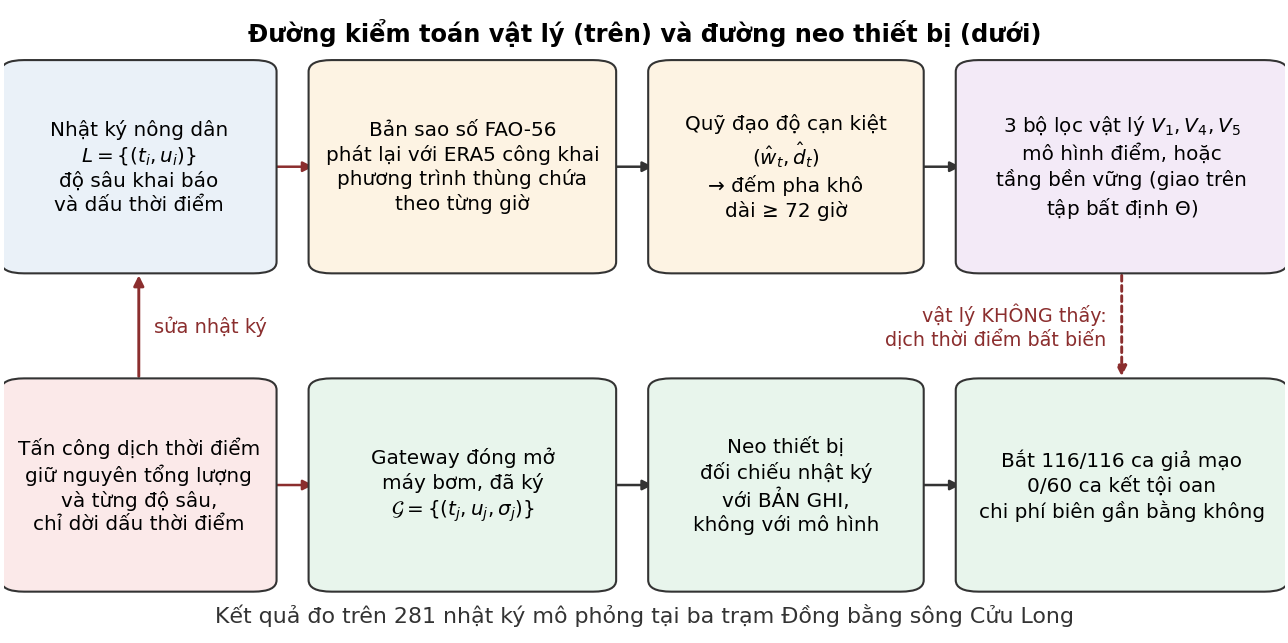
\includegraphics[height=6.9cm]{figures/fig1_method.png}
\caption{Đường đi của dữ liệu trong phương pháp. Lớp kiểm toán vật lý phát lại nhật ký khai báo qua bản sao số cân bằng nước rồi đi qua ba bộ lọc; lớp neo thiết bị đối chiếu cùng nhật ký đó với bản ghi lệnh có chữ ký của gateway. Mũi tên đứt cho thấy tấn công dịch thời điểm đi qua lớp vật lý mà không bị phát hiện.}\label{fig:method}
\end{figure}

% BAN TIENG VIET cua 02_threat_attack.tex — viet lai 2026-10-12 theo academic-prose.
% Moi con so, cite, label, ref, equation giu NGUYEN so voi ban truoc.
% Thuat ngu theo glossary.tex. KHONG them/bot claim.
\section{Mô hình đe doạ}
\label{sec:threat}

Một nhật ký tưới khai báo là một ánh xạ hữu hạn
\begin{equation}
L=\{(t_i,u_i)\}_{i=1}^{|L|},\qquad u_i>0,\ t_i\in[0,T),
\label{eq:log}
\end{equation}
trong đó:
\begin{symbolist}
\item[$L$] nhật ký khai báo của một vụ, gồm các lần tưới mà nông dân đã ghi;
\item[$|L|$] số lần tưới có trong nhật ký;
\item[$u_i$] độ sâu khai báo của lần tưới thứ $i$, tức lượng nước nông dân ghi đã
  tưới vào thửa ruộng, tính bằng milimét. Đây là độ dày lớp nước nếu trải đều lượng
  nước đó trên mặt ruộng, chứ không phải độ sâu của nước ngầm hay độ sâu tầng đất;
  đại lượng này cùng đơn vị với sức chứa ẩm đồng ruộng $FC$ và lượng nước trong tầng
  rễ $w_t$ đã định nghĩa ở Mục~\ref{sec:model};
\item[$t_i$] chỉ số giờ của lần tưới thứ $i$, nhận giá trị trong khoảng từ 0 đến
  $T$ đã định nghĩa ở Mục~\ref{sec:model}.
\end{symbolist}
Bên gian lận có thể làm giả ba đại lượng độc lập, và mỗi tầng phòng thủ chỉ quan sát
một tập con trong số đó:
\begin{equation}
\underbrace{\textstyle\sum_i u_i}_{\text{tổng lượng}}\,,\qquad
\underbrace{\{u_i\}}_{\text{từng độ sâu tưới}}\,,\qquad
\underbrace{\{t_i\}}_{\text{dấu thời gian}}\,.
\label{eq:three}
\end{equation}
Bảng~S1 của Phụ lục liệt kê các lớp gian lận tương ứng với từng đại lượng. Ở đây \emph{bên gian lận} (adversary) là bên nộp nhật ký có chủ ý làm sai lệch số liệu,
có thể là chính nông dân hoặc người vận hành ghi thay cho nông dân; bài này không suy
đoán động cơ và không giả định bên đó thuộc nhóm người nào, mà chỉ mô hình hoá hành vi
của bên đó. Chúng tôi giả định bên gian lận \emph{duy lý}, nghĩa là nó tối đa hoá
số pha khô được cấp tín chỉ với điều kiện không bị đánh dấu. Chúng tôi giả định bên gian lận biết đầy đủ bộ phát hiện, vì nó được định nghĩa ngay
trong bài này và mã nguồn được công khai. Vì vậy
$\varepsilon$ trong \eqref{eq:v4} dưới đây không phải là một tham số bí mật, mà
là dung sai công bố cho sai số mô hình và được đặt bằng $5$~mm trong toàn bộ thí
nghiệm, đúng bằng giá trị trong mã nguồn công khai. Tham số này khác với ngưỡng
chênh lệch bơm $\tau_0$ ở Mục~\ref{sec:guarantee}.

Tầng phòng thủ thứ nhất đối chiếu tổng lượng nước khai báo với tổng lượng nước
thật sự đã bơm. Gọi $M$ là lượng nước thật sự đã bơm, đo tại trạm bơm của hợp tác
xã, và gọi $U(L)=\sum_i u_i$ là tổng lượng mà nhật ký khai báo. Tầng~1 dùng thống
kê chênh lệch
\begin{equation}
G=M-U(L),
\label{eq:gap}
\end{equation}
trong đó:
\begin{symbolist}
\item[$G$] chênh lệch bơm, tính bằng mm, là lượng nước bơm thật vượt quá tổng
  lượng đã khai báo;
\item[$M$] tổng lượng nước thật sự đã bơm trong vụ, đo tại trạm của hợp tác xã,
  tính bằng mm;
\item[$U(L)$] tổng các độ sâu khai báo trong nhật ký $L$, tính bằng mm.
\end{symbolist}

$G$ dương nghĩa là nông dân khai thiếu. Tuy nhiên đại lượng quyết định tín chỉ
không phải $G$ mà là \emph{số pha khô}. Ký hiệu
$\mathcal{A}(\cdot)$ là tập các quãng liền nhau dài nhất có thể $[a,b)$ trên một
quỹ đạo phát lại, trong đó độ cạn kiệt luôn đạt từ $d_{\mathrm{dry}}$ trở lên,
không có khai báo tưới nào, và mỗi quãng kéo dài ít nhất $72$~giờ, tức mức tối thiểu ba ngày theo
Quyết định 4801~\cite{qd4801}:
\begin{equation}
\begin{aligned}
\mathcal{A}\bigl(\{\hat d_t\}\bigr)=\Bigl\{[a,b):\ &\min_{t\in[a,b)}
\hat d_t\ge d_{\mathrm{dry}},\\
&u_t=0\ \forall t\in[a,b),\\
&b-a\ge 72\,\mathrm{h}\Bigr\}.
\end{aligned}
\label{eq:awd}
\end{equation}
trong đó:
\begin{symbolist}
\item[$\mathcal{A}(\cdot)$] toán tử trả về tập các pha khô đủ điều kiện cấp tín
  chỉ của một quỹ đạo độ cạn kiệt;
\item[$[a,b)$] một quãng giờ liền nhau, bắt đầu tại giờ $a$ và kết thúc trước giờ
  $b$, là quãng dài nhất thoả điều kiện nên không thể mở rộng thêm;
\item[$\hat d_t$] độ cạn kiệt tại giờ $t$ suy ra từ nhật ký, đã định nghĩa ở
  Mục~\ref{sec:model};
\item[$d_{\mathrm{dry}}$] ngưỡng cạn kiệt tối thiểu để một quãng được coi là pha
  khô, là phân số không thứ nguyên;
\item[$u_t$] độ sâu tưới áp dụng tại giờ $t$, bằng 0 trong suốt quãng khô;
\item[$b-a$] độ dài của quãng, tính bằng giờ.
\end{symbolist}

Khi đó số pha được cấp tín chỉ là
\begin{equation}
n_{\mathrm{dry}}(L)=\bigl|\mathcal{A}\bigl(\mathcal{R}(L)\bigr)\bigr|,
\label{eq:ndry}
\end{equation}
trong đó $n_{\mathrm{dry}}(L)$ là số pha khô được cấp tín chỉ của nhật ký $L$, còn
$\mathcal{R}(L)$ là quỹ đạo phát lại của nhật ký đó theo \eqref{eq:replay}, và ký
hiệu $|\cdot|$ đếm số phần tử của tập. Ngưỡng $d_{\mathrm{dry}}=0{,}45$ được dùng
chung cho toàn bài. Giá trị này là một lựa chọn mô hình hoá của chúng tôi, đặt đủ cao để một pha khô thực sự có ý nghĩa
chứ không chỉ là ruộng hơi ẩm; độ nhạy của nó được khảo sát ở Phụ lục~S20.
Doanh thu của nông dân tỉ lệ với $n_{\mathrm{dry}}$ chứ không tỉ lệ với $U(L)$,
và chính sự phân biệt này khiến tấn công ở Mục~\ref{sec:timeshift} mang lại lợi
ích tín chỉ mà vẫn vô hình trước mọi quy tắc chỉ đối chiếu tổng lượng khai báo
với tổng lượng bơm thật.

\section{Các bộ lọc dựa trên vật lý và điểm mù chính xác của chúng}
\label{sec:filters}

Phát lại $L$ với dữ liệu ERA5 công khai cho ra $(\hat w_t,\hat d_t)$; bản thảo chưa công bố nêu trên~\cite{twingate2026} trình bày đầy đủ cân bằng nước này. Trên nền đó có
ba bộ lọc được áp dụng.

trong đó $V_1(L)$ là tập chỉ số của những lần khai báo bị bộ lọc thứ nhất đánh dấu,
còn $\hat w_{t_i}^{-}$ là lượng nước tầng rễ ngay trước khi áp dụng lần khai báo
thứ $i$, đã định nghĩa ở Mục~\ref{sec:model}.

Bộ lọc \emph{$V_4$} (vượt sức chứa) đánh dấu mọi khai báo vượt quá phần thiếu hụt
tại giờ đó, vì lượng dư hoặc đã chảy tràn hoặc đã thấm mất, nên không thể coi là
``đã được áp dụng'' theo nghĩa mà quy chuẩn đòi hỏi:
\begin{equation}
V_4(L)=\{\,i:\ u_i\ >\ \underbrace{(FC-\hat w_{t_i}^{-})}_{\text{phần thiếu hụt}}
\ +\ \varepsilon\,\}.
\label{eq:v4}
\end{equation}

trong đó $V_4(L)$ là tập chỉ số các lần khai báo bị đánh dấu, và biểu thức trong
dấu ngoặc ôm là phần thiếu hụt, tức lượng nước mà tầng rễ còn tiếp nhận được tại
giờ đó trước khi chạm sức chứa ẩm đồng ruộng.

Bộ lọc \emph{$V_5$} (giới hạn thấm) không phụ thuộc vào trạng thái tầng rễ, mà
chỉ áp dụng ràng buộc rằng một lần tưới kéo dài $\tau_i$ không thể cấp nhiều hơn
lượng nước mà đất thực sự tiếp nhận được:
\begin{equation}
u_i\ \le\ k_{\mathrm{inf}}\,\tau_i+p_{\max},
\label{eq:v5}
\end{equation}
với $k_{\mathrm{inf}}=10$~mm\,h$^{-1}$ và $p_{\max}=100$~mm, lấy ở đầu rộng của dải giá
trị đã công bố cho ruộng lúa làm dầm~\cite{kukal2004,bouman2001}, tức giới hạn
$110$~mm tại $\tau_i=1$~giờ. Chúng tôi chọn đầu rộng như vậy để một nông dân gộp
hai lần tưới liền kề vào cùng một giờ không bị kết tội oan.


trong đó:
\begin{symbolist}
\item[$\tau_i$] thời gian kéo dài của lần tưới thứ $i$, tính bằng giờ;
\item[$k_{\mathrm{inf}}$] tốc độ thấm tối đa của ruộng, tính bằng mm mỗi giờ;
\item[$p_{\max}$] lượng nước tối đa mà ruộng nhận được trong một trận tưới bất
    kể thời gian, tính bằng mm.
\end{symbolist}

Bộ lọc thứ ba, vốn đánh dấu độ cạn kiệt xuống dưới điểm héo, không thể kích hoạt
trên lúa vụ khô đồng bằng; bằng chứng ở Ghi chú~\ref{sec:v2reach}. Cách đánh số $V_1$, $V_4$, $V_5$ theo bản thảo chưa công bố nêu trên; bài này không dùng $V_2$ và $V_3$.

\begin{proposition}[Điểm mù chính xác của các phòng thủ tổng hợp]
\label{prop:blind}
Giả sử $L$ và $L'$ có cùng đa tập hợp các độ sâu và cùng tổng lượng, tức
$\{u_i\}=\{u'_j\}$ theo nghĩa đa tập hợp. Khi đó
\begin{equation}
G(L)=G(L')\qquad\text{và}\qquad |V_5(L)|=|V_5(L')|.
\end{equation}
\end{proposition}

\begin{proof}
Xem Phụ lục~S11; cả hai đại lượng đều là hàm đối xứng của đa tập hợp độ sâu và
không bao giờ phụ thuộc $t_i$.
\end{proof}

Mệnh đề~\ref{prop:blind} gói trọn toàn bộ khó khăn trong một dòng. Hai phòng thủ không phụ thuộc việc mô hình có đúng hay không, tức quy tắc đối
chiếu tổng lượng bơm thật $G$ ở \eqref{eq:gap} và giới hạn thấm $V_5$, đều bất
biến \emph{chính xác} dưới phép dịch thời điểm mà bên gian lận cần. Hai
bộ lọc còn lại là $V_1$ và $V_4$, vốn phụ thuộc thứ tự qua $\hat w_{t_i}^{-}$,
nhưng cả hai cũng không giúp được gì.

\section{Tấn công dịch thời điểm}
\label{sec:timeshift}

\begin{proposition}[Lợi ích tín chỉ và sự lọt lưới là cùng một hành động]
\label{prop:coincide}
Giả sử một khai báo tại giờ $t$ có phần thiếu hụt $c_t=FC-\hat w_t^{-}$. Giữa hai khai báo liên tiếp, thùng chứa mất đi
$\Delta_t=\sum_{s}(\mathit{ETc}_s+\mathit{DP}_s-P_s^{+})\ge 0$, nên việc hoãn
một khai báo thêm $\delta$ giờ làm tăng phần thiếu hụt của nó đúng bằng lượng
nước đã thoát đi trong các giờ đó:
\begin{equation}
c_{t+\delta}\ \ge\ c_t+\min\!\bigl(\delta\cdot\overline{\Delta},\ FC-\hat w_t^{-}\bigr).
\label{eq:delay}
\end{equation}
trong đó:
\begin{symbolist}
\item[$c_t$] phần thiếu hụt tại giờ $t$, tính bằng mm, bằng lượng nước mà tầng rễ
  còn tiếp nhận được trước khi chạm sức chứa ẩm đồng ruộng;
\item[$\Delta_t$] lượng nước mà thùng chứa mất đi giữa hai lần khai báo liên tiếp,
  tính bằng mm;
\item[$\mathit{ETc}_s$] bốc thoát hơi nước của cây trồng tại giờ $s$, chính là
  $ET_{c,s}$ của \eqref{eq:etc};
\item[$\mathit{DP}_s$] lượng thấm sâu xuống dưới tầng rễ tại giờ $s$, là phần
  nước bị toán tử cắt bỏ loại đi trong \eqref{eq:bucket};
\item[$P_s^{+}$] lượng mưa thực sự đi vào ruộng tại giờ $s$, sau khi đã trừ dòng
  chảy mặt $RO_s$;
\item[$\delta$] số giờ mà một khai báo bị hoãn lại;
\item[$\overline{\Delta}$] lượng nước mất đi trung bình mỗi giờ trong quãng chờ.
\end{symbolist}

Cả ba số hạng của $\Delta_t$ đều lấy từ cùng phương trình thùng chứa
\eqref{eq:bucket}, nên bất đẳng thức này không dựa trên giả định thuỷ văn nào mới.
Nghĩa là khi một lệnh tưới bị ghi muộn, ruộng khô thêm trong quãng chờ nên số pha
khô tăng, còn đất khô hơn lại hấp thụ đúng lượng nước đó, nên không bộ lọc vật lý
nào thấy bất thường.

Do đó phép biến đổi dời các khai báo \emph{ra khỏi} một khoảng khô và đặt lên
biên của khoảng đó đồng thời (i)~làm tăng $n_{\mathrm{dry}}$, vì khoảng đó
không còn bị ngắt quãng, và (ii)~làm tăng $c_t$ tại mỗi khai báo bị dời, điều
mà theo \eqref{eq:v4} khiến $V_4$ \emph{ít} có khả năng kích hoạt hơn. Bên gian lận không phải đánh đổi điều gì. Gradient của lợi nhuận và gradient của sự
không thể phát hiện cùng chỉ một hướng.
\end{proposition}

\begin{proof}
Xem Phụ lục~S11. Nói ngắn gọn, (i) đúng theo định nghĩa, vì $\mathcal{A}$ đòi
hỏi không có khai báo nào bên trong khoảng; (ii) suy ra được vì hoãn một khai
báo để thùng chứa tiếp tục thoát nước thêm $\delta$ giờ mà không có dòng vào,
nên phần thiếu hụt chỉ có thể tăng trong khi $u_i$ không đổi.
\end{proof}

Vì vậy không thể bịt tấn công này bằng một mô hình thuỷ văn tốt hơn. Do đó, mọi bộ phát hiện mà phán quyết chỉ phụ thuộc vào quỹ đạo phát lại đều buộc
phải tích phân đúng lượng nước đã thoát đi trong thời gian chờ, chính là lượng
nước làm cho khai báo bị hoãn trở nên hợp lý về mặt vật lý. Trên
thực nghiệm chúng tôi cài đặt tấn công bằng một thuật toán leo đồi dò từng bước, mỗi bước thử dịch một lệnh tưới sang giờ khác trong khoảng
$[-36,36]$ giờ, và chỉ giữ bước dịch đó khi tổng lượng nước không đổi đến từng
chữ số, mọi độ sâu vẫn nằm dưới \eqref{eq:v5} và $n_{\mathrm{dry}}$ tăng nghiêm
ngặt. Tấn công này không ăn cắp nước mà đánh cắp \emph{lịch sử} (Phụ lục~S19).


% BAN TIENG VIET cua 03_guarantee.tex — viet lai 2026-10-12 theo academic-prose.
% Moi con so, cite, label, ref, equation giu NGUYEN so voi ban truoc.
% Thuat ngu theo glossary.tex. KHONG them/bot claim.
\section{Khi nào được kết tội một nông dân?}
\label{sec:guarantee}

Hai mục trước cho thấy lớp kiểm toán vật lý vừa bỏ lọt bên gian lận tinh vi vừa có nguy
cơ kết tội oan người trung thực. Mục này xử lý vế thứ hai trước khi tổng hợp thành khẳng định điểm mù không thể tránh.

\subsection{Độ sâu tưới chấp nhận được là một dải, không phải một con số}
\label{sec:umax}

Nếu chỉ lấy giới hạn từ một hồ sơ đất và một điều kiện đầu duy nhất thì cách
tính cho ra đúng một con số, $u\le 61$~mm, là khai báo lớn nhất không bao giờ
gây báo động. Vì $V_4$ kích hoạt khi $u_i>c_{t_i}+\varepsilon$ và
$c_t=d_t\cdot\mathrm{span}$, giới hạn tại một ruộng có độ cạn kiệt ban đầu
$w_0$ và tưới không muộn hơn $d^{*}$ là
\begin{equation}
u_{\max}=\max(d^{*},w_0)\cdot\mathrm{span}+\varepsilon .
\label{eq:umax}
\end{equation}
trong đó:
\begin{symbolist}
\item[$u_{\max}$] độ sâu khai báo lớn nhất, tính bằng mm, mà bộ lọc không bao giờ đánh dấu;
\item[$d^{*}$] độ cạn kiệt tại giờ tưới muộn nhất được xét, là phân số không thứ nguyên;
\item[$w_0$] độ cạn kiệt ban đầu của ruộng, cùng đơn vị phân số;
\item[$\mathrm{span}$] biên độ của thang cạn kiệt, bằng $FC-WP$ tính bằng mm, đã định nghĩa ở Mục~\ref{sec:model};
\item[$\varepsilon$] dung sai công bố cho sai số mô hình, bằng $5$~mm như ở Mục~\ref{sec:filters}.
\end{symbolist}

Giới hạn này được viết theo tỷ lệ cạn kiệt quy về tầng rễ chứ không theo một
cao độ tuyệt đối, nên khác với các ngưỡng mực nước tuyệt đối đang dùng trong thực
hành, nó không trôi khi mặt ruộng sụt lún; mệnh đề và độ dịch đo được cho đồng bằng
ở Phụ lục~S4.

Từ đây rút ra hai điều chỉnh, cả hai đều được kiểm chứng bằng cách quét toán tử
phát lại chứ không chỉ bằng đại số (dẫn xuất ở Phụ lục~S14). Thứ nhất,
\eqref{eq:umax} dùng $\max$ chứ không dùng hiệu, nên một ruộng khô ban đầu lại
chấp nhận khai báo \emph{lớn hơn} một ruộng ướt, còn biểu thức dạng hiệu thì
không tương ứng với trạng thái vật lý nào. Thứ hai, giới hạn này chỉ chặn một
\emph{lần tưới đơn lẻ} chứ không chặn cả vụ, nên một bên gian lận phát nhiều khai báo
dưới ngưỡng có thể thổi phồng tổng lượng mà không bị giới hạn nào chặn lại.
Bảng~S2 của Phụ lục đưa ra dải cần được báo cáo thay thế, $[49{,}0; 86{,}0]$~mm
trên toàn $\Theta$.

\subsection{Chỉ kết tội khi mọi kịch bản mô hình đều cho thấy vi phạm}
\label{sec:robust}

Kiểm toán viên không biết đất của nông dân, không biết giai đoạn sinh trưởng và
cũng không biết hiệu suất của hệ thống dẫn nước. Gọi $\Theta$ là tập bất định và
$V_\theta(L)$ là tập vi phạm dưới cấu hình $\theta$. Bộ phát hiện mô hình điểm
chỉ đánh giá một $\theta_0$ mặc định rồi coi mọi vi phạm là có tội. Chúng tôi
thay nó bằng một phép giao:
\begin{equation}
\begin{aligned}
V_{\mathrm{rob}}(L)&=\bigcap_{\theta\in\Theta}V_\theta(L),\\
\Theta&=\mathcal{S}\times\mathcal{K}\times\mathcal{E}\times\mathcal{W},
\end{aligned}
\label{eq:robust}
\end{equation}
trong đó:
\begin{symbolist}
\item[$V_{\mathrm{rob}}(L)$] tập vi phạm bền vững của nhật ký $L$, chỉ khác rỗng khi $L$ vi phạm dưới mọi cấu hình;
\item[$\Theta$] tập bất định, là tích của bốn tập thành phần dưới đây;
\item[$\mathcal{S}$] tập loại đất, gồm $5$ loại;
\item[$\mathcal{K}$] tập chế độ hệ số cây trồng, gồm $2$ chế độ;
\item[$\mathcal{E}$] tập mức hiệu suất tưới, gồm $3$ mức;
\item[$\mathcal{W}$] tập trạng thái đầu, gồm $5$ trạng thái.
\end{symbolist}

Do đó $|\Theta|=150$ và mỗi nhật ký tốn $150$ lần phát lại. Ngữ nghĩa của phán quyết được chọn cố ý lệch về phía bảo vệ nông dân, tức ưu tiên
tránh kết tội oan hơn là tối đa năng lực phát hiện:
\begin{equation}
a(L)=
\begin{cases}
\text{kết tội}, & V_{\mathrm{rob}}(L)\neq\emptyset,\\
\text{chờ xác minh}, & \text{trường hợp còn lại}.
\end{cases}
\label{eq:verdict}
\end{equation}
trong đó $a(L)$ là phán quyết dành cho nhật ký $L$. Phán quyết ``chờ xác minh''
nghĩa là phải xác minh thêm tại thực địa, chứ hệ thống không tự kết luận gian lận.

\begin{proposition}[Không kết tội oan trong $\Theta$]
\label{prop:noalarm}
Nếu cấu hình thật của ruộng $\theta^{*}$ thuộc $\Theta$ và $L$ tuân thủ dưới
$\theta^{*}$, thì $V_{\mathrm{rob}}(L)=\emptyset$ và nông dân không bị kết tội.
\end{proposition}

\begin{proof}
$V_{\mathrm{rob}}(L)\subseteq V_{\theta^{*}}(L)=\emptyset$.
\end{proof}

Mệnh đề~\ref{prop:noalarm} là cơ sở để lớp này triển khai được trong thực tế. Sai
số mô hình có thể làm giảm năng lực phát hiện nhưng không thể tạo ra một lời kết
tội oan, và cái giá phải trả cho đảm bảo đó được nêu rõ ở phần sau. Hai chi tiết cài đặt có thể âm thầm phá vỡ mệnh đề nếu làm sai, đó là cách xử lý
những cấu hình trong tập bất định mà tại đó không bộ lọc nào kích hoạt, và độ trải
của tập trạng thái đầu $\mathcal{W}$ (Phụ lục~S7).

\subsection{Ngưỡng chênh lệch bơm tỉ lệ thuận}

Quy tắc tuyệt đối $G>\tau_0$ với $\tau_0=5$~mm ngầm giả định nhật ký là bản sao
trung thực của lượng nước đã bơm. Giả định này không đúng, vì quên ghi, làm tròn
đến $5$~mm gần nhất và ghi trễ một ngày đều làm tăng $G$ mà không hề có hành vi
sai trái nào. Vì vậy ngưỡng phải co giãn theo số lần tưới được ghi:
\begin{equation}
\begin{aligned}
\tau(n)&=\delta_{\mathrm{rel}}M+z\sqrt{n}\,\sigma_{\mathrm{event}},\\
\sigma_{\mathrm{event}}^{2}&=p(1-p)\bar u^{2}+\tfrac{r^{2}}{12}
+q(1-q)(s\bar u)^{2},
\end{aligned}
\label{eq:tau}
\end{equation}
trong đó:
\begin{symbolist}
\item[$\tau(n)$] ngưỡng chênh lệch bơm cho phép, tính bằng mm, khi nhật ký có $n$ lần tưới;
\item[$n$] số lần tưới được ghi trong nhật ký;
\item[$\delta_{\mathrm{rel}}$] tỷ lệ sai lệch tương đối cho phép trên lượng bơm thật $M$, bằng $2\%$;
\item[$z$] hệ số nhân của độ lệch chuẩn, đặt bằng $3$;
\item[$\sigma_{\mathrm{event}}$] độ lệch chuẩn của sai số ghi chép trên mỗi lần tưới, tính bằng mm;
\item[$p$] tỷ lệ quên ghi một lần tưới;
\item[$r$] bước làm tròn độ sâu, bằng $5$~mm;
\item[$q$] tỷ lệ ghi sai độ sâu, và $s$ là biên độ tương đối của lỗi đó;
\item[$\bar u$] độ sâu điển hình của một lần tưới, bằng $30$~mm.
\end{symbolist} Quy tắc tuyệt đối là trường hợp suy biến
$n\to0$, $\sigma_{\mathrm{event}}\to0$.

\begin{remark}[Bộ lọc thứ ba không bao giờ kích hoạt được]
\label{sec:v2reach}
Lớp vật lý có ba bộ lọc, nhưng bộ thứ ba --- đánh dấu ruộng cạn kiệt xuống dưới
điểm héo --- không bao giờ kích hoạt được, vì hai lý do độc lập. Lý do thứ nhất
thuộc về cách cài đặt: ngưỡng của nó là $1{,}02$, trong khi chỉ số được báo cáo đã
bị cắt ngọn về một đoạn cố định, nên điều kiện không thể nào đúng và bộ lọc có $0$
lần kích hoạt trong cả $281$ nhật ký. Lý do thứ hai thuộc về thực tế đồng ruộng:
chúng tôi sửa lỗi đó bằng cách dùng độ cạn kiệt chưa cắt ngọn, rồi đo lại trên
$150$ cấu hình với nhật ký rỗng, tức điều kiện khô hạn nhất có thể, thì giá trị này
cũng chỉ đạt đỉnh $0{,}9987$. Nghĩa là một ruộng lúa vụ khô ở đồng bằng không cạn
tới mức chạm điểm héo (Bảng~S3 của Phụ lục, dẫn xuất ở S13). Bộ lọc này vì vậy chỉ
là một chốt an toàn chống trạng thái vô lý, không phải bằng chứng về năng lực phát
hiện, và lớp này chỉ có hai bộ lọc vật lý thực sự hoạt động.
\end{remark}


% BAN TIENG VIET cua 04_anchor.tex — viet lai 2026-10-12 theo academic-prose.
% Moi con so, cite, label, ref, equation giu NGUYEN so voi ban truoc.
% Thuat ngu theo glossary.tex. KHONG them/bot claim.
\section{Chứng thực neo theo thiết bị}
\label{sec:anchor}

\subsection{Bản ghi của gateway}

Các mệnh đề~\ref{prop:blind}--\ref{prop:coincide} cho thấy tổng lượng và từng độ
sâu vẫn chưa đủ, còn thứ tự thời gian mới đúng là thứ bên gian lận thao túng. Vì vậy, bất kỳ cơ chế kiểm toán nào muốn chặn được tấn công này đều phải quan sát
dấu thời gian, mà bên duy nhất có thể bảo chứng cho một dấu thời gian là thiết bị
đã thực thi lệnh đó. Giả sử gateway giữ một bản ghi
lệnh có chữ ký
\begin{equation}
\mathcal{G}=\{(t_j,u_j,\sigma_j)\},
\label{eq:gateway}
\end{equation}
trong đó:
\begin{symbolist}
\item[$\mathcal{G}$] bản ghi lệnh của gateway, gồm mọi lệnh đóng mở máy bơm trong vụ;
\item[$t_j$] giờ mà bộ điều khiển đóng máy bơm ở lệnh thứ $j$;
\item[$u_j$] độ sâu nước mà bộ điều khiển đã cấp ở lệnh đó, tính bằng mm;
\item[$\sigma_j$] chữ ký số trên cặp $(t_j,u_j)$, do bộ điều khiển tạo ra tại thời điểm đóng mở máy bơm.
\end{symbolist}

Phép thử neo đối chiếu nhật ký khai báo với bản ghi đó:
\begin{equation}
\begin{aligned}
\Delta_{\mathrm{time}}&=\{t_i\}\triangle\{t_j\},\\
\Delta_{\mathrm{depth}}&=\max_{t}\bigl|u(t)-u_{\mathcal{G}}(t)\bigr|,
\end{aligned}
\label{eq:deltas}
\end{equation}
trong đó:
\begin{symbolist}
\item[$\Delta_{\mathrm{time}}$] tập các giờ có mặt ở bản ghi này nhưng vắng ở bản ghi kia;
\item[$\triangle$] phép hiệu đối xứng giữa hai tập giờ, trả về các phần tử chỉ thuộc một trong hai tập;
\item[$u(t)$] độ sâu khai báo tại giờ $t$ trong nhật ký $L$;
\item[$u_{\mathcal{G}}(t)$] độ sâu mà gateway ghi nhận tại cùng giờ $t$;
\item[$\Delta_{\mathrm{depth}}$] độ lệch lớn nhất giữa hai độ sâu, lấy trên các giờ có mặt ở cả hai bản ghi.
\end{symbolist}

Phán quyết khi đó là
\begin{equation}
A(L,\mathcal{G})=
\begin{cases}
\text{giả mạo}, & \Delta_{\mathrm{time}}\neq\emptyset
\ \vee\ \Delta_{\mathrm{depth}}>\epsilon,\\
\text{khớp}, & \text{trường hợp còn lại},
\end{cases}
\label{eq:anchor}
\end{equation}
trong đó:
\begin{symbolist}
\item[$A(L,\mathcal{G})$] phán quyết của phép thử neo đối với nhật ký $L$;
\item[$\epsilon$] dung sai so khớp độ sâu, bằng $10^{-6}$~mm, tức khớp chính xác tới mức nhiễu dấu phẩy động;
\item[$\vee$] phép hoặc logic, nghĩa là chỉ cần một trong hai loại sai lệch là đủ kết luận giả mạo.
\end{symbolist} Cần
gọi tên riêng hai loại sai lệch, vì dịch thời điểm chỉ làm thay đổi
$\Delta_{\mathrm{time}}$, thổi phồng độ sâu chỉ làm thay đổi
$\Delta_{\mathrm{depth}}$, còn bỏ sót và thêm mới thì làm thay đổi cả hai. Nhờ
vậy một phép đối chiếu duy nhất bắt được mọi lớp gian lận.

\begin{proposition}[Tính đầy đủ của neo thiết bị]
\label{prop:complete}
Nếu nhật ký khai báo $L$ khác bản ghi gateway $\mathcal{G}$ về đa tập hợp các
giờ hoặc về bất kỳ độ sâu nào tại một giờ chung, thì $A(L,\mathcal{G})$ trả về
\text{giả mạo}. Nếu $L$ và $\mathcal{G}$ khớp cả hai, thì $L$ là một bản sao
trung thực và không có sự giả mạo nào đối với ba đại lượng trong
\eqref{eq:three}.
\end{proposition}

\begin{proof}
Xem Phụ lục~S12. Mệnh đề thứ nhất là định nghĩa của \eqref{eq:anchor}, còn mệnh
đề thứ hai suy ra được vì cả ba đại lượng có thể làm giả đều là hàm của tập giờ
và các độ sâu theo giờ.
\end{proof}

\subsection{Vì sao neo thiết bị không dẫn tới kết tội oan}

Điểm hoá giải là neo thiết bị đối chiếu một bản sao với \emph{nguồn} chứ không đối chiếu
một nhật ký với một \emph{mô hình}: nguồn sự thật là bản ghi của gateway chứ không phải
trí nhớ của nông dân, nên nhật ký chỉ là một góc nhìn của bản ghi mà thiết bị đã giữ. Nếu
nhật ký bỏ sót một lệnh có trong $\mathcal{G}$ thì đó là lỗi ghi chép và mục đó được bổ
sung từ $\mathcal{G}$; còn nếu nhật ký khai thêm một lệnh không có trong $\mathcal{G}$,
hoặc khai sai thời điểm hay độ sâu so với $\mathcal{G}$, thì theo \eqref{eq:anchor} đó là
giả mạo. Khi đó phép thử neo chỉ có thể kết tội oan một nông dân trung thực nếu bản ghi
của gateway tự mâu thuẫn với chính nó, và đó là bài toán bảo đảm toàn vẹn thiết bị chứ
không còn là bài toán kiểm toán nhật ký. Nhờ vậy Bảng~\ref{tab:falseacc} giữ ở mức
$0/60$, trong khi các bộ phát hiện dựa trên quỹ đạo phát lại vẫn kết tội oan ở mức
$26{,}7\%$ và $5{,}0\%$ (Phụ lục~S18).

\subsection{Chi phí và phạm vi của tuyên bố}

Neo thiết bị yêu cầu dùng gateway trong bản thảo chưa công bố nêu trên~\cite{twingate2026}, thiết bị vốn đóng mở máy bơm và ghi lại bản ghi lệnh có chữ ký kèm dấu thời gian
như một phần của chức năng an toàn. Chi phí biên của việc chứng thực chỉ gồm lưu trữ và truyền đi một bản ghi vốn đã được gateway sinh ra trong quá trình hoạt động bình thường (Bảng~S4 của Phụ lục).

Tuy vậy, phạm vi áp dụng của tuyên bố hẹp hơn kỳ vọng mà phần mở đầu gợi ra. Một nhật ký viết tay, không có thiết bị nào tham gia vào vòng ghi nhận, thì bản
thân nó \emph{không} tạo thành bằng chứng được chấp nhận, vì
Mục~\ref{sec:results-attack} đo được một bên gian lận duy lý có thể thổi phồng tín chỉ
thêm $+35\%$ mà vẫn lọt qua mọi phép thử dựa trên vật lý và tổng lượng ($6/6$
nhật ký bị sửa). Vì vậy MRV với chi phí \emph{biên} gần như bằng không chỉ
khả thi ở nơi có một bộ điều khiển đứng giữa nông dân và máy bơm, còn ở nơi tưới
thủ công thì lớp này không áp dụng được.


% BAN TIENG VIET cua 05_design_results.tex — viet lai 2026-10-12 theo academic-prose.
% Moi con so, cite, label, ref giu NGUYEN so voi ban truoc.
% Thuat ngu theo glossary.tex. KHONG them/bot claim.
\section{Thiết kế thực nghiệm}
\label{sec:design}

Thiết kế thực nghiệm so sánh bốn tầng phòng thủ trên chín loại nhật ký, dùng một thửa
ruộng cố ý vi phạm mọi giả định của bản sao số, vì nếu thửa ruộng do chính bản sao số sinh
ra thì tỷ lệ $0/60$ ca kết tội oan chỉ đo tính tự nhất quán chứ không đo năng lực thật
(Phụ lục~S10.4). Thửa ruộng ở đây do một tiến trình riêng biệt sinh ra, khác bản sao số
theo bảy trục, mỗi trục đều có nguồn đã công bố; mọi giá trị nằm ở Bảng~S5 của Phụ lục,
còn danh sách từng trục và ngữ nghĩa ghi chép theo sự kiện ở S20.1.

Dữ liệu thời tiết là ERA5 theo giờ~\cite{hersbach2020} lấy từ kho lưu trữ
Open-Meteo cho ba trạm Cần Thơ, Sóc Trăng và Cà Mau, trong năm khan nước 2024 và năm thừa nước 2025. Cửa sổ mô phỏng chạy từ ngày 1 tháng Ba đến ngày 29
tháng Năm, tức $2\,160$~giờ, đúng mùa khô mà AWD được áp dụng~\cite{tuong2003}.

Bốn tầng phòng thủ được cài đặt như sau. Tầng~1 là bộ phát hiện mô hình điểm với
hồ sơ mặc định và ngưỡng tuyệt đối $\tau_0=5$~mm. Tầng~2 là bộ phát hiện bền vững
của \eqref{eq:robust} kết hợp ngưỡng tỉ lệ của \eqref{eq:tau}, chạy trên cả
$\Theta$ rút gọn, với $24$ lần phát lại mỗi nhật ký và $10$ hạt giống ngẫu nhiên,
lẫn $\Theta$ đầy đủ, gồm $150$ lần phát lại có kiểm chéo. Tầng~3 là neo thiết bị của
\eqref{eq:anchor}. Tầng~4 chỉ dùng vật lý và đóng vai trò mốc so sánh.

Trong chín loại nhật ký thì hai loại là nhật ký trung thực, gồm điều kiện giấy và điều
kiện ruộng, ba loại là giả mạo ngây thơ và bốn loại là đối kháng, được dựng bằng một bộ
tối ưu chứ không theo một công thức cố định (danh sách đầy đủ ở S16). Mọi thống kê tấn
công đều được tính có điều kiện trên những nhật ký thật sự bị sửa, vì hai cạm bẫy của bộ
khung thử nghiệm được ghi ở S10.2. Thứ nhất, một bên gian lận không tìm được nước đi cải
thiện sẽ trả lại nhật ký mà không sửa gì, nên nếu đếm vô điều kiện thì số ``tấn công bị
bắt'' sẽ gồm cả những ca không hề có tấn công. Thứ hai, mỗi biến thể phải được so với mốc
của chính nó, vì nhật ký trung thực điều kiện giấy do một lần sinh riêng tạo ra.

Với mỗi tầng, chúng tôi báo cáo tỷ lệ lọt lưới, tức số nhật ký giả mà không tầng
vật lý nào đánh dấu, và tỷ lệ kết tội oan trên nhật ký trung thực. Về tác động
tín chỉ, chúng tôi báo cáo $n_{\mathrm{dry}}$ của \eqref{eq:ndry} theo ghép cặp
so với mốc ruộng trung thực. Tổng lượng nước chỉ được dùng để chẩn đoán (S10.3).

\section{Kết quả}
\label{sec:results}

Kết quả dưới đây trả lời ba câu hỏi theo thứ tự, gồm bộ phát hiện mặc định có an
toàn không, vật lý có nhìn thấy tấn công sinh lợi không, và neo thiết bị có bịt
được khoảng trống đó không.

\subsection{Bộ phát hiện mô hình điểm không chỉ lạc quan mà còn kết tội oan}

Bảng~\ref{tab:falseacc} đưa ra kết quả phủ định trung tâm của bài. Trên nhật ký điều
kiện giấy, như đã giải thích ở phần Mở đầu, bộ phát hiện mô hình điểm không kết tội ai và
tái hiện đúng con số $0/60$ của giao thức tự nhất quán (Phụ lục~S10.4), nhưng trên nhật
ký điều kiện ruộng thì nó kết tội oan $26{,}7\%$ nông dân trung thực. Nguyên nhân nằm ở
\eqref{eq:gap} khi dùng một ngưỡng tuyệt đối, vì quên ghi, làm tròn hoặc ghi trễ một ngày
đều tạo ra $G>5$~mm mà không có hành vi sai trái nào; chênh lệch đo được trên nhật ký
trung thực điều kiện ruộng lên tới $65$~mm. Ngưỡng tỉ lệ của \eqref{eq:tau} hạ tỷ lệ oan
xuống $5{,}0\%$, còn neo thiết bị hạ xuống $0/60$.

\subsection{Vật lý không nhìn thấy tấn công sinh lợi}
\label{sec:results-attack}

\begin{figure}[!t]
\centering
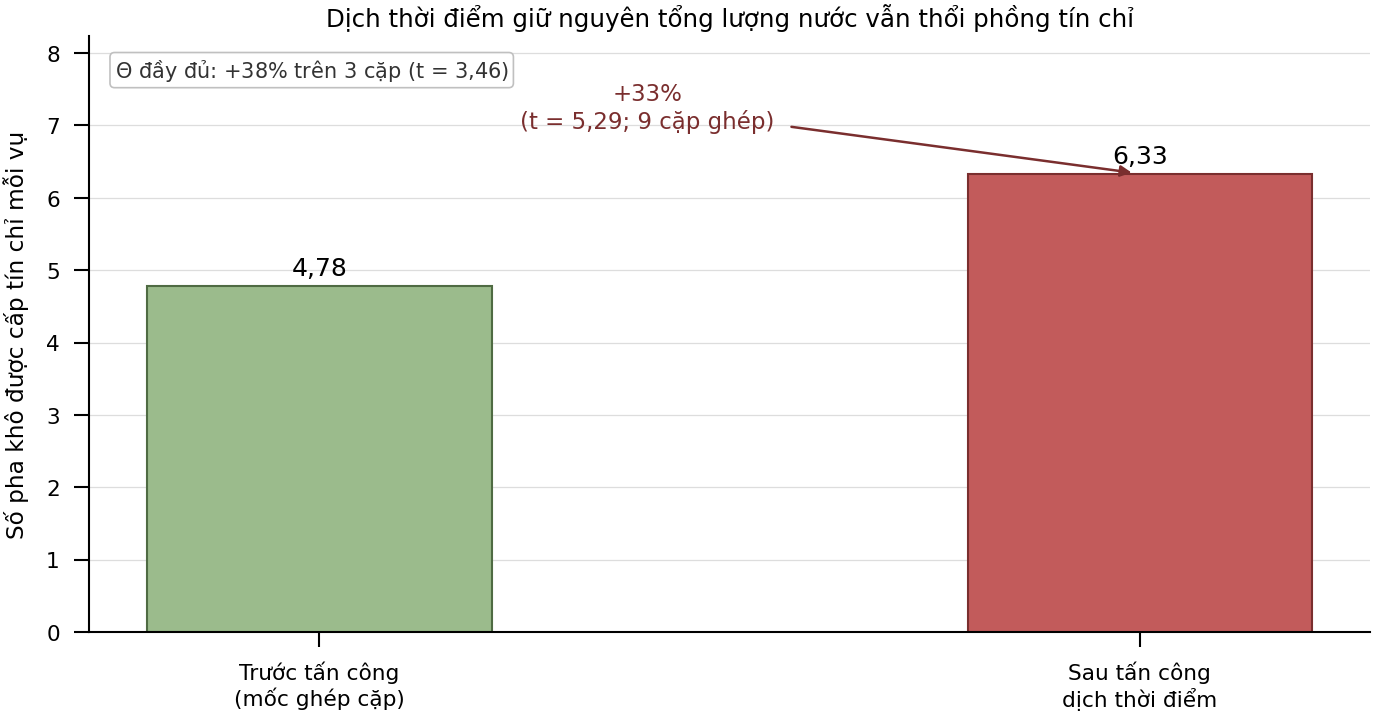
\includegraphics[height=6.9cm]{figures/fig3_timeshift.png}
\caption{Tấn công dịch thời điểm trên tập ghép cặp. Số pha khô được cấp tín chỉ trước và sau khi dời thời điểm lệnh, còn tổng lượng nước và từng độ sâu được giữ nguyên. Mức tăng trên tập bất định đầy đủ được ghi ở góc dưới bên phải.}\label{fig:timeshift}
\end{figure}

Hình~\ref{fig:timeshift} vẽ lại phép so sánh ghép cặp đó. Bảng~\ref{tab:credit} là kết quả phủ định thứ hai và là kết quả quan trọng về mặt
kinh tế. Mọi con số thổi phồng trong bảng đều là so sánh \emph{ghép cặp}, tức đối chiếu
mỗi nhật ký bị sửa với nhật ký trung thực của cùng một quỹ đạo và cùng một thửa
ruộng, và chỉ tính trên các tấn công thật sự thay đổi bản
ghi, vì cách tính không ghép cặp sẽ phóng đại lợi ích lên khoảng hai lần (S15).

Dịch thời điểm nâng số pha khô được cấp tín chỉ từ $4{,}78$ lên $6{,}33$ mỗi vụ, tức
$+33\%$ trên chín nhật ký bị sửa ($t=5{,}29$). Với tập bất định đầy đủ, mức tăng là $+38\%$
trên ba nhật ký ($t=3{,}46$, $p=0{,}074$), cùng định hướng nhưng chưa đạt mức ý nghĩa
$0{,}05$ ở cỡ mẫu này. Bên gian lận duy lý đạt $+35\%$ và $+40\%$ ($p=0{,}007$ và $p=0{,}30$).
Gộp khai báo hầu như không thu được gì khi ghép cặp ($+1\%$, $+2\%$), còn hai kiểu giả mạo
thô sơ thậm chí \emph{làm giảm} số pha khô được cấp tín chỉ ($-1\%$, $-17\%$). Chỉ phép
hoán vị dấu thời điểm giữ nguyên tổng lượng nước mới sinh lợi, đúng như
Mệnh đề~\ref{prop:coincide} dự đoán.

Tỷ lệ lọt lưới trong Bảng~\ref{tab:defence} là phần cốt lõi của kết quả. Dịch thời điểm
lọt qua tầng vật lý bền vững ở $8$ trong $9$ nhật ký bị sửa, còn bên gian lận duy lý lọt ở $6$
trong $6$. Mô hình điểm bắt được nhiều hơn ($4$ trong $9$), nhưng chính nó kết tội oan
$26{,}7\%$ nông dân trung thực; tầng bền vững hạ tỷ lệ oan xuống $5{,}0\%$ thì giao phần
lớn khả năng phát hiện về tay bên gian lận ($1$ trong $9$). \emph{Không cấu hình vật lý nào
thoát khỏi sự đánh đổi đó}, vì cả hai tầng đều là hàm của quỹ đạo phát lại. Bộ lọc thấm
$V_5$ kích hoạt $648$ lần nhưng chỉ trên kiểu giả mạo thổi phồng độ sâu thô sơ, nên nó
hữu ích và trực giao với mối đe doạ sinh lợi.

\begin{figure}[!t]
\centering
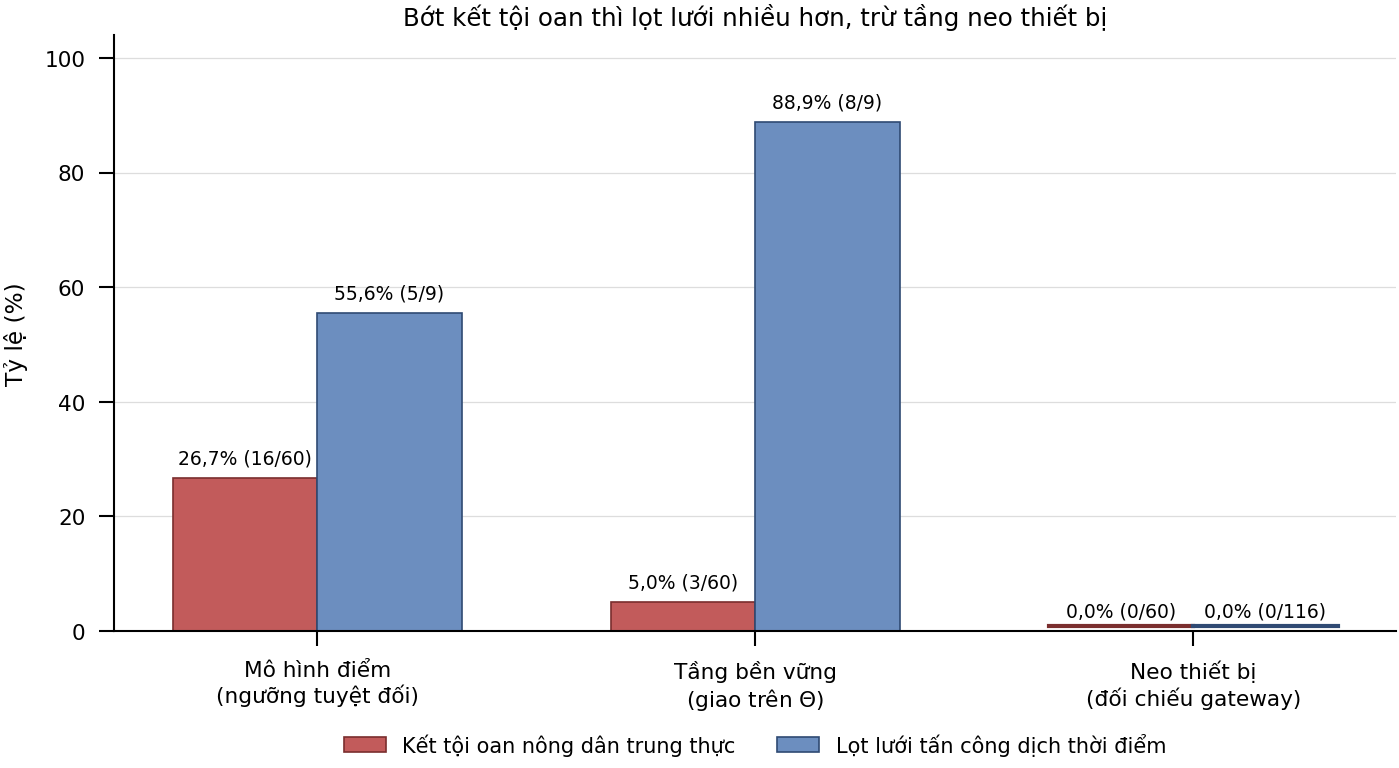
\includegraphics[height=6.9cm]{figures/fig2_tradeoff.png}
\caption{Sự đánh đổi giữa hai loại sai sót theo ba tầng phòng thủ. Giảm tỷ lệ kết tội oan nông dân trung thực thì tăng tỷ lệ lọt lưới tấn công dịch thời điểm; chỉ tầng neo thiết bị đạt cả hai bằng không.}\label{fig:tradeoff}
\end{figure}

\subsection{Neo thiết bị bịt mọi lớp gian lận, và cái giá phải trả}

Hình~\ref{fig:tradeoff} tóm tắt sự đánh đổi mà hai mục trên đã đo. Bảng~\ref{tab:defence} cũng đưa ra kết quả xây dựng của bài. Toàn bộ $281$ nhật ký được
kiểm toán bằng tập bất định rút gọn, trong đó $85$ nhật ký được kiểm toán lại bằng tập
đầy đủ (Phụ lục~S17.2). Trong $281$ nhật ký có $116$ nhật ký thật sự bị sửa; neo thiết bị
bắt được $116/116$ và không kết tội oan nhật ký nào trong $60$ nhật ký trung thực điều
kiện ruộng ($37/37$ và $0/18$ với $\Theta$ đầy đủ). Giả mạo ngây thơ bị mọi tầng bắt được,
nên khác biệt giữa các tầng chỉ nằm ở các dòng đối kháng, nơi cả bộ phát hiện bền vững lẫn
quy tắc đối chiếu tổng lượng đều bỏ lọt và chỉ neo thiết bị bắt được.

Tính bền vững không đạt được mà không có đánh đổi: trên chín nhật ký gian lận bỏ sót
thật sự bị sửa, mô hình điểm bắt được $9/9$ trong khi quy tắc bền vững chỉ bắt $4/9$
($4/4$ so với $2/4$ ở $\Theta$ đầy đủ). Đây là một sự suy giảm năng lực phát hiện chứ
không phải cải thiện Pareto, dù chúng tôi cho rằng lợi ích ở phía tránh kết tội oan lớn
hơn tổn thất ở phía phát hiện. Mọi kết luận đều đúng với cả $\Theta$ rút gọn, gồm $24$
lần phát lại trên $281$ nhật ký với $10$ hạt giống ngẫu nhiên, lẫn $\Theta$ đầy đủ, gồm
$150$ lần phát lại trên $85$ nhật ký với $3$ hạt giống ngẫu nhiên, cụ thể là kết tội oan
$0/60$ và $0/18$, tính đầy đủ của neo $116/116$ và $37/37$, lọt lưới dịch thời điểm $8/9$
và $3/3$, thổi phồng ghép cặp $+33\%$ và $+38\%$ (Phụ lục~S17).

\begin{table}[!t]
\centering
\caption{Kết tội oan trên nhật ký trung thực, thuộc tính then chốt mà phương án này
được quảng bá. Điều kiện giấy tái hiện kết quả $0/60$ của giao thức tự nhất quán;
điều kiện ruộng phơi bày ngưỡng chênh lệch tuyệt đối.}
\label{tab:falseacc}
\footnotesize
% Sinh TU DONG tu tables/tab_false_accusation.tex (ban tieng Anh, von sinh tu outputs/*.csv)
% boi experiments/make_tables_hujos_vi.py. KHONG sua tay.
% Nhan dich qua bang tra cuong che; so chi doi dinh dang sang kieu Viet Nam (dau phay thap phan).
% Da assert: cung so dong, cung so vach, cung tap chu so voi ban EN.

% Sinh TU DONG tu outputs/eval_theta_*.csv boi experiments/make_tables_anchored.py
% KHONG sua tay: moi con so deu truy nguon duoc ve CSV.

\fittocol{%
\begin{tabular}{@{}>{\raggedright\arraybackslash}p{4.20cm}>{\raggedright\arraybackslash}p{2.10cm}>{\raggedright\arraybackslash}p{2.10cm}@{}}
\toprule
Lớp phòng thủ & Trung thực, điều kiện giấy & Trung thực, điều kiện ruộng \\
\midrule
Mô hình điểm, chỉ vật lý & 0/60 & 2/60 \\
Mô hình điểm với ngưỡng tuyệt đối ($G>5$\,mm) & 0/60 & 16/60 \\
Quy tắc bền vững ($\forall$ trên $\Theta$), chỉ vật lý & 0/60 & 0/60 \\
Quy tắc bền vững với $\tau(n)$ tỉ lệ & 0/60 & 3/60 \\
Bản ghi lệnh neo theo thiết bị & 0/60 & 0/60 \\
\bottomrule
\end{tabular}
}

\end{table}

\begin{table}[!t]
\centering
\caption{Số pha khô được cấp tín chỉ dài ít nhất $72$~giờ, tức mức tối thiểu ba ngày không tưới lại theo Quyết định 4801, và cũng là đại lượng mà VM0051 dùng để tính tín chỉ; so với mốc ruộng trung thực, tính theo ghép cặp. Cột cuối đếm số tấn công thật sự sửa nhật ký. Bảng có hai mốc. Dòng ``trung
thực'' là trung bình $3{,}23$ pha của toàn bộ $60$ nhật ký trung thực, còn cột
``trước'' của mỗi dòng gian lận là nhật ký trung thực \emph{ghép cặp} cùng trạm,
năm, seed và loại đất ($4{,}87$ với các biến thể đối kháng). Hai mốc khác nhau
có chủ đích, xem Phụ lục~S15.}
\label{tab:credit}
\footnotesize
% Sinh TU DONG tu tables/tab_credit.tex (ban tieng Anh, von sinh tu outputs/*.csv)
% boi experiments/make_tables_hujos_vi.py. KHONG sua tay.
% Nhan dich qua bang tra cuong che; so chi doi dinh dang sang kieu Viet Nam (dau phay thap phan).
% Da assert: cung so dong, cung so vach, cung tap chu so voi ban EN.

% Sinh TU DONG tu outputs/eval_theta_*.csv boi experiments/make_tables_anchored.py
% KHONG sua tay: moi con so deu truy nguon duoc ve CSV.

\fittocol{%
\begin{tabular}{@{}>{\raggedright\arraybackslash}p{2.90cm}c>{\raggedright\arraybackslash}p{1.90cm}cc@{}}
\toprule
Loại nhật ký & Nhật ký bị sửa & Pha khô ghép cặp (trước $\to$ sau) & Thổi phồng & $t$ \\
\midrule
Nông dân trung thực (điều kiện ruộng) & --- & 3,23 (mốc) & mốc & --- \\
Thêm lệnh tưới & 23/23 & 4,87 $\to$ 4,83 & -1\% & -0,57 \\
Độ sâu khai không khả thi & 23/23 & 4,87 $\to$ 4,04 & -17\% & -4,03 \\
Bỏ sót lệnh thật & 9/23 & 5,44 $\to$ 4,78 & -12\% & -2,83 \\
Gộp khai báo, 24 h & 23/23 & 4,87 $\to$ 4,91 & +1\% & 0,37 \\
Gộp khai báo, 96 h & 23/23 & 4,87 $\to$ 4,96 & +2\% & 0,62 \\
Dịch thời điểm (duy lý) & 9/23 & 4,78 $\to$ 6,33 & +33\% & 5,29 \\
Bên gian lận duy lý & 6/23 & 4,33 $\to$ 5,83 & +35\% & 4,39 \\
\bottomrule
\end{tabular}
}

\end{table}

\begin{table}[!t]
\centering
\caption{Kết quả chính. Mọi tỷ lệ được tính trên các nhật ký mà tấn công
\emph{thật sự} sửa; cột thứ hai báo số bị sửa trên số được sinh, vì bên gian lận trả lại nhật ký mà không sửa gì khi không tìm được nước đi cải thiện. Tỷ lệ lọt lưới là
phần mà không tầng vật lý nào đánh dấu.}
\label{tab:defence}
\footnotesize
% Sinh TU DONG tu tables/tab_defence.tex (ban tieng Anh, von sinh tu outputs/*.csv)
% boi experiments/make_tables_hujos_vi.py. KHONG sua tay.
% Nhan dich qua bang tra cuong che; so chi doi dinh dang sang kieu Viet Nam (dau phay thap phan).
% Da assert: cung so dong, cung so vach, cung tap chu so voi ban EN.

% Sinh TU DONG tu outputs/eval_theta_*.csv boi experiments/make_tables_anchored.py
% KHONG sua tay: moi con so deu truy nguon duoc ve CSV.

\fittocol{%
\begin{tabular}{@{}>{\raggedright\arraybackslash}p{2.85cm}c>{\raggedright\arraybackslash}p{1.30cm}>{\raggedright\arraybackslash}p{1.50cm}>{\raggedright\arraybackslash}p{1.45cm}@{}}
\toprule
Biến thể gian lận & Nhật ký bị sửa & Lọt mô hình điểm & Lọt bộ phát hiện bền vững & Neo thiết bị bắt \\
\midrule
Nông dân trung thực (điều kiện ruộng) & 0/60 (trung thực) & \textbf{27\%} bị oan & 5\% bị oan & 0\% bị oan \\
Thêm lệnh tưới & 23/23 & 0\% & 0\% & 23/23 \\
Độ sâu khai không khả thi & 23/23 & 0\% & 0\% & 23/23 \\
Bỏ sót lệnh thật & 9/23 & 0\% & 56\% & 9/9 \\
Gộp khai báo, 24 h & 23/23 & 39\% & 91\% & 23/23 \\
Gộp khai báo, 96 h & 23/23 & 39\% & 91\% & 23/23 \\
Dịch thời điểm (duy lý) & 9/23 & 56\% & 89\% & 9/9 \\
Bên gian lận duy lý & 6/23 & 100\% & 100\% & 6/6 \\
\midrule
\textbf{Mọi nhật ký thật sự giả} & \textbf{116} & \textbf{---} & \textbf{---} & \textbf{116/116} \\
\bottomrule
\end{tabular}
}

\end{table}

% Bang benchmark: so sanh voi cac phuong an MRV da cong bo (SOTA).
% So sinh tu experiments/benchmark_confirmation.py -> _benchmark_summary.json
% KHONG sua tay; nhan dich boi make_tables_hujos_vi.py tu bang EN.
\begin{table}[!t]
\centering
\caption{Số pha khô đủ điều kiện cấp tín chỉ có thể xác nhận được theo từng
phương án MRV, trên $150$ pha có thật trong $60$ ruộng mô phỏng; một pha chỉ
được tính nếu có ít nhất một lần quan sát rơi vào trong nó. Hai dòng cuối có cùng giá trị ở chỉ số này, khác nhau ở chi phí và ở điều chúng chứng
minh được với một nhật ký đã bị sửa.}
\label{tab:benchmark}
\footnotesize
% Sinh TU DONG tu tables/tab_benchmark.tex (ban tieng Anh, von sinh tu outputs/*.csv)
% boi experiments/make_tables_hujos_vi.py. KHONG sua tay.
% Nhan dich qua bang tra cuong che; so chi doi dinh dang sang kieu Viet Nam (dau phay thap phan).
% Da assert: cung so dong, cung so vach, cung tap chu so voi ban EN.

% Sinh TU DONG tu outputs/_benchmark_summary.json boi experiments/make_table_benchmark.py
% KHONG sua tay: moi con so truy nguon ve benchmark_confirmation.py.

\fittocol{
\begin{tabular}{@{}>{\raggedright\arraybackslash}p{4.30cm}ccc@{}}
\toprule
Phương án xác minh & Pha khô xác nhận được ($n=150$) & Số lần quan sát mỗi vụ & Thiết bị mỗi thửa \\
\midrule
Ảnh + tự khai (thực hành hiện hành)~\cite{qd4801} & 0/150 (0\%) & --- & 0 (ống PVC) \\
Sentinel-1A+1B (chu kỳ 6 ngày)~\cite{hashemi2022s1} & 124/150 (83\%) & 15 & 0 \\
Sentinel-1A đơn lẻ (chu kỳ 12 ngày)~\cite{clauss2017s1} & 90/150 (60\%) & 8 & 0 \\
Ống đo mực nước liên tục (IoT)~\cite{delacruz2022} & 150/150 (100\%) & 2.153 & 1 mỗi thửa \\
Bản ghi lệnh có chữ ký (bài này)~\cite{twingate2026} & 150/150 (100\%) & 2.153 & 0 (bộ điều khiển) \\
\bottomrule
\end{tabular}
}

\end{table}

% BAN TIENG VIET cua 06_discussion_conclusion.tex — viet lai 2026-10-12 theo academic-prose.
% Moi con so, cite, label, ref giu NGUYEN so voi ban truoc.
% Thuat ngu theo glossary.tex. KHONG them/bot claim.
\section{Bàn luận}
\label{sec:discussion}

\subsection{Quan hệ với các công trình trước}

Việc giám sát AWD đã được tiếp cận theo ba hướng, gồm cảm biến mực nước gắn thiết bị
đo~\cite{delacruz2022}, viễn thám~\cite{lovell2019,islam2026alose,mlrice2025,narayanan2024},
và MRV ở cấp chương trình~\cite{qd1490,mae2026progress,irri2026mrv}. Song song
đó, phân tích tổng hợp nông học~\cite{carrijo2017} cùng các nghiên cứu về tiếp
nhận~\cite{lampayan2015,enriquez2021} giải thích vì sao giám sát có thiết bị
không lan rộng được. Tuy nhiên không hướng nào đánh giá \emph{độ tin cậy của
chính bản ghi hành động}, và đó là câu hỏi mà bài báo đặt ra; khảo sát đầy đủ ở
Phụ lục~S8.

Đối với radar vệ tinh, vốn là phương án chi phí thấp hiển nhiên, chúng tôi đo khả
năng xác nhận pha khô chứ không tranh luận về tính khả thi của nó. Bảng~\ref{tab:benchmark} chấm điểm mọi phương án theo số pha khô đủ điều kiện cấp tín
chỉ mà phương án đó xác nhận được trong $150$ pha khô có thật trên $60$ thửa ruộng mô
phỏng (Phụ lục~S9.2), trong đó một pha chỉ được tính khi có ít nhất một lần quan sát
rơi vào bên trong nó~\cite{clauss2017s1,hashemi2022s1,delacruz2022}.

Có hai điểm cần thận trọng khi đọc bảng này. Thứ nhất, cột này đo khả năng
\emph{kiếm} tín chỉ chứ không đo khả năng phát hiện gian lận. Thứ hai, ống đo và
bản ghi lệnh cùng đạt $100\%$ nhưng khác nhau về chi phí và về thứ chúng chứng
minh được, còn ảnh chụp kèm tự khai chỉ đạt $0\%$ vì nó không tạo ra chuỗi quan
sát nào để đối chiếu. Vì vậy radar vẫn giữ vai trò mà Phụ lục 4 của VM0051 giao
cho nó, tức một phép kiểm chéo theo thửa làm giảm tần suất kiểm tra thực
địa~\cite{vm0051} (Phụ lục~S9.2).

\subsection{Giới hạn}

Bảy giới hạn thu hẹp phạm vi các tuyên bố của bài, tất cả đều được phát biểu đầy đủ
ở Phụ lục~S21, trong đó hai giới hạn ảnh hưởng trực tiếp tới các kết quả chính được
nêu ở đây.

Giới hạn thứ nhất là nông dân được mô phỏng. Các bản giả mạo được tiêm vào quỹ
đạo mô phỏng, nên vẫn cần một thử nghiệm thực địa để đo phản ứng hành vi, trước
hết là liệu nông dân có thay đổi việc bơm \emph{thật sự} của mình một khi biết
có neo thiết bị hay không. Đó là kiểu tấn công làm thay đổi $M$ chứ không thay
đổi $L$, và mô hình của chúng tôi không biểu diễn được nó.

Giới hạn thứ hai là tấn công chỉ được minh hoạ trong năm khan nước. Năm 2025, phần lớn
nhật ký rơi xuống dưới mức tối thiểu ba lệnh, vì phải có từ ba lệnh trở lên thì việc hoán
vị thời điểm giữa chúng mới tạo ra được một cấu hình khai báo khác có lợi, nên trong $37$
nhật ký thật sự bị sửa ở $\Theta$ đầy đủ thì cả $37$ đều thuộc năm 2024. Chính sự khác biệt
giữa hai năm đó đã là một kết quả đáng chú ý, vì nó cho thấy rủi ro gian lận MRV tập trung
ở những nơi khan nước, nhưng kết quả tấn công chưa đủ để kết luận cho một mùa mưa. Ở
$\Theta$ rút gọn có mười hai nhật ký bị sửa thuộc năm 2025 và chúng hành xử giống nhau, đủ
để gợi ý chứ chưa đủ để kết luận. Năm giới hạn còn lại ở S21.

\section{Kết luận}

Chúng tôi khởi đầu với mục tiêu làm cho MRV lúa gần như miễn phí bằng cách kiểm
toán một nhật ký tưới do nông dân tự ghi đối chiếu với vật lý nước trong đất.
Trên thửa ruộng do chính mô hình kiểm toán sinh ra, lớp đó báo cáo không kết tội oan
và phát hiện trọn vẹn, nhưng như đã giải thích ở phần Mở đầu, cả hai con số đều là
sản phẩm của một giao thức tự nhất quán. Việc dựng lại thửa ruộng trước một bên gian lận
tối ưu hoá đại lượng được cấp tín chỉ đã làm thay đổi kết luận.

Bộ phát hiện mô hình điểm kết tội oan $26{,}7\%$ nông dân trung thực. Ngưỡng tỉ lệ kết hợp
phép giao trên tập bất định hạ con số đó xuống $5{,}0\%$, còn phép neo thiết bị giữ $0/60$,
với cái giá đo được về năng lực phát hiện: $9/9$ xuống $4/9$ ở gian lận bỏ sót. Các con số
này đo trên $281$ nhật ký với tập bất định rút gọn gồm $24$ lần phát lại; trên tập đầy đủ
$150$ lần phát lại, cả tầng bền vững lẫn phép neo đều giữ $0/18$ ca kết tội oan. Ngược lại, một phép
hoán vị thời điểm khai báo giữ nguyên tổng lượng nước thổi phồng số pha khô được cấp tín
chỉ thêm $33\%$ (ghép cặp, $p<0{,}001$) và lọt qua tầng bền vững ở $8$ trong $9$ cùng $3$
trong $3$ nhật ký bị sửa; trên tập bất định đầy đủ mức tăng là $38\%$ nhưng chỉ với ba nhật
ký nên chưa đạt mức ý nghĩa. Không cấu hình vật lý nào thoát khỏi đánh đổi đó, vì hoãn một
khai báo vừa kéo dài pha khô vừa tăng phần thiếu hụt dành cho nó, nên lợi nhuận và sự
không thể phát hiện dùng chung một gradient.

Vì vậy cách khắc phục không nằm ở thuỷ văn. Đối chiếu nhật ký khai báo với bản ghi lệnh có
chữ ký và dấu thời gian của gateway bắt được $116/116$ nhật ký thật sự bị giả mạo, không
kết tội oan nhật ký nào trong $60$ nhật ký trung thực, và chi phí không vượt quá một bộ điều khiển mà bản thảo chưa công bố nêu trên đã triển khai. Vật lý \emph{ràng buộc}
một nhật ký, nhưng chỉ bản ghi thiết bị có chữ ký mới \emph{chứng thực} được nó, nên MRV
với chi phí \emph{biên} gần như bằng không chỉ khả thi ở nơi có thiết bị đứng giữa nông
dân và máy bơm.

Phân tích cũng để lại ba hệ quả thực hành cho lớp kiểm toán vật lý đã nêu ở phần Mở
đầu, gồm độ sâu tưới chấp nhận được là một dải $[49{,}0; 86{,}0]$~mm chứ không phải
một giá trị $61$~mm, bộ lọc thứ ba bất động, và phép thử chênh lệch tuyệt đối là
không thể chấp nhận. Mã nguồn, cả hai tập bất định, toàn bộ $281$ nhật ký đã kiểm toán và
$46$ phép thử đơn vị đều được công khai.


% ---------------------------------------------------------------- khai bao
\section*{Dữ liệu, mã nguồn và tuyên bố}

Mã nguồn, cả hai tập bất định, cả hai cấu hình bên gian lận và toàn bộ $281$ nhật ký
đã kiểm toán có tại \url{https://github.com/mxuanvan02/TwinGate} theo giấy phép MIT; dữ liệu khí tượng là tái phân tích ERA5 công khai qua kho lưu trữ
Open-Meteo. Nghiên cứu này được tài trợ bởi Đại học Huế trong đề tài mã số
DHH2025-19-07. Các tác giả tuyên bố không có xung đột lợi ích. Không áp dụng phê duyệt đạo đức vì nghiên cứu chỉ dùng dữ liệu tái phân tích công khai và thí
nghiệm mô phỏng, không có người tham gia, động vật hay can thiệp thực địa.

% ---------------------------------------------------------------- tai lieu
% LOI DA SUA (batch 17): \renewcommand{\thetable}{S\arabic{table}} nam o FRONT MATTER
% cua supplementary_vi.tex, KHONG nam trong supplementary_body.tex -> khi nhung vao bai chinh,
% bang phu luc danh so tiep 4 bang cua than bai. Do that: .aux ban gop cho
% tab:baseline=8, tab:setup=9 va PDF in 'Bảng 8. Chi phí MRV…', 'Bảng 9. Cấu hình thực
% nghiệm.' trong khi van ben canh van viet 'Bảng~S4 của Phụ lục' -> caption va tham
% chieu lech nhau. Fix: dat lai counter + nhan S ngay truoc khi nhung, de ban gop in
% dung 'Bang S1..S5' giong het ban phu luc rieng. Da probe trong /tmp: .aux -> S4/S5,
% 'Bảng 8/9' = 0 lan, 4 bang than bai van 1..4, 0 loi, so trang khong doi.
% \clearpage: phu luc la khoi tai lieu rieng, phai bat dau trang moi. Do that: truoc
% day S1 nam o dong 5/37 cua trang 20, dinh ngay sau cau ve phe duyet dao duc.
\clearpage
\appendix
\setcounter{table}{0}
\renewcommand{\thetable}{S\arabic{table}}
% LOI DA SUA (batch 17): XUNG DOT SO MENH DE trong phu luc rieng. Phu luc co
% proposition RIENG (prop:subsid trong sections/08_subsidence) va remark rieng
% (sections/09_cost). \newtheorem dung counter rieng nen truoc day prop:subsid in ra
% 'Mệnh đề 1' — trong khi CUNG PDF nay viet 'bị mù theo Mệnh đề 1 của bài chính'
% (stub r@prop:blind=1) va S11 la 'Chứng minh Mệnh đề 1 và Mệnh đề 2'. Nhan
% 'Mệnh đề 1' tro HAI menh de khac nhau trong mot tai lieu.
% Bai chinh co 4 menh de (blind=1, coincide=2, noalarm=3, complete=4) va 1 ghi chu,
% nen dat counter tiep noi => prop:subsid=5, remark=2: DUNG BANG so ma ban gop
% (main + supplementary_body) da in ra. Idempotent trong ban gop vi counter da
% o 4/1 khi bat dau phu luc.
% Dat o DAY (khong phai supplementary_vi.tex) vi gate check_supp_vi_numbers doc
% supplementary_body.tex cho ban VI va supplementary.tex cho ban EN; dat o file gate khong
% doc se lam EN thua 2 so -> gate bao lech gia.
\setcounter{proposition}{4}
\setcounter{remark}{1}

\section*{S1. Các lớp gian lận và mỗi tầng phòng thủ quan sát được gì}

\begin{minipage}{\textwidth}\footnotesize
\captionof{table}{Ba đại lượng làm giả được của \eqref{eq:three} trong bài chính và lớp gian lận
nào làm thay đổi từng đại lượng. ``đúng'' nghĩa là đại lượng đó được giữ nguyên, nên tầng
phòng thủ tương ứng bị mù theo Mệnh đề~\ref{prop:blind} của bài chính.}
% Sinh TU DONG tu tables/tab_threat.tex (ban tieng Anh, von sinh tu outputs/*.csv)
% boi experiments/make_tables_hujos_vi.py. KHONG sua tay.
% Nhan dich qua bang tra cuong che; so chi doi dinh dang sang kieu Viet Nam (dau phay thap phan).
% Da assert: cung so dong, cung so vach, cung tap chu so voi ban EN.

% Sinh TU DONG tu outputs/eval_theta_*.csv boi experiments/make_tables_anchored.py
% KHONG sua tay: moi con so deu truy nguon duoc ve CSV.

\fittocol{%
\begin{tabular}{@{}>{\raggedright\arraybackslash}p{2.85cm}>{\raggedright\arraybackslash}p{0.95cm}>{\raggedright\arraybackslash}p{1.05cm}>{\raggedright\arraybackslash}p{0.95cm}>{\raggedright\arraybackslash}p{2.20cm}@{}}
\toprule
Biến thể gian lận & Tổng mm & Từng độ sâu & Thời điểm & Làm giả cái gì \\
\midrule
Nông dân trung thực (điều kiện ruộng) & đúng & đúng & đúng & Mốc: bảy trục khác biệt thực tế đang bật \\
Thêm lệnh tưới & SAI & đúng & đúng & Thổi phồng hồ sơ hoạt động quản lý \\
Độ sâu khai không khả thi & SAI & SAI & đúng & Một phần ba số mục đặt bằng toàn bộ dung tích chứa \\
Bỏ sót lệnh thật & SAI & đúng & đúng & Xoá cửa sổ 96 h để tạo ra một pha khô \\
Gộp khai báo, 24 h & đúng & thay đổi & SAI & Cùng lượng nước, ít lần tưới hơn và lớn hơn \\
Gộp khai báo, 96 h & đúng & thay đổi & SAI & Cùng lượng nước, các lần tưới bám vào lưới thô \\
Dịch thời điểm (duy lý) & đúng & đúng & SAI & Leo đồi theo từng giờ để tối đa số pha khô được cấp tín chỉ \\
Bên gian lận duy lý & đúng & đúng & SAI & Chọn cửa sổ gộp làm tối đa số pha khô \\
\bottomrule
\end{tabular}
}

\end{minipage}

% ---------------------------------------------------------------- S2
\section*{S2. Biên độ sâu tưới chấp nhận được trên toàn $\Theta$}

\begin{minipage}{\textwidth}\footnotesize
\captionof{table}{Biên độ sâu tưới chấp nhận được $u_{\max}$ (\eqref{eq:umax} trong bài chính)
trên toàn dải của FAO-56 Bảng 2. Giá trị đơn lẻ $61$\,mm ban đầu chỉ là một dòng của bảng này.}
% Sinh TU DONG tu tables/tab_umax.tex (ban tieng Anh, von sinh tu outputs/*.csv)
% boi experiments/make_tables_hujos_vi.py. KHONG sua tay.
% Nhan dich qua bang tra cuong che; so chi doi dinh dang sang kieu Viet Nam (dau phay thap phan).
% Da assert: cung so dong, cung so vach, cung tap chu so voi ban EN.

% Sinh TU DONG tu outputs/eval_theta_*.csv boi experiments/make_tables_anchored.py
% KHONG sua tay: moi con so deu truy nguon duoc ve CSV.

\fittocol{%
\begin{tabular}{@{}>{\raggedright\arraybackslash}p{3.00cm}>{\raggedright\arraybackslash}p{1.25cm}>{\raggedright\arraybackslash}p{1.85cm}>{\raggedright\arraybackslash}p{1.85cm}@{}}
\toprule
Loại đất (FAO-56 Bảng 2) & Biên độ (mm) & $u_{\max}$ tại $w_0=0$ & $u_{\max}$ tại $w_0=0{,}90$ \\
\midrule
đất thịt pha cát & 55,0 & 49,0 & 54,5 \\
đất thịt & 75,0 & 65,0 & 72,5 \\
đất thịt pha limon & 90,0 & 77,0 & 86,0 \\
đất thịt pha sét limon & 70,0 & 61,0 & 68,0 \\
đất sét & 80,0 & 69,0 & 77,0 \\
\midrule
\textbf{Dải phải công bố} & --- & \textbf{49,0} & \textbf{86,0} \\
\bottomrule
\end{tabular}
}

\end{minipage}

% ---------------------------------------------------------------- S3
\section*{S3. Khả năng kích hoạt của bộ lọc điểm héo}

\begin{minipage}{\textwidth}\footnotesize
\captionof{table}{Khả năng kích hoạt của bộ lọc điểm héo trên $150$ cấu hình với nhật ký rỗng, tức
điều kiện thời tiết khô hạn nhất có được.}
% Sinh TU DONG tu tables/tab_f2_unreachable.tex (ban tieng Anh, von sinh tu outputs/*.csv)
% boi experiments/make_tables_hujos_vi.py. KHONG sua tay.
% Nhan dich qua bang tra cuong che; so chi doi dinh dang sang kieu Viet Nam (dau phay thap phan).
% Da assert: cung so dong, cung so vach, cung tap chu so voi ban EN.

% Sinh TU DONG tu outputs/eval_theta_*.csv boi experiments/make_tables_anchored.py
% KHONG sua tay: moi con so deu truy nguon duoc ve CSV.

\fittocol{%
\begin{tabular}{@{}>{\raggedright\arraybackslash}p{1.55cm}c>{\raggedright\arraybackslash}p{1.75cm}>{\raggedright\arraybackslash}p{0.85cm}>{\raggedright\arraybackslash}p{2.60cm}@{}}
\toprule
Trạm & Năm & Cạn kiệt cắt ngọn lớn nhất & $V_2$ kích hoạt & Diễn giải \\
\midrule
Cần Thơ & 2024 & 0,998 & 0 & không bao giờ xuống dưới điểm héo \\
Cần Thơ & 2025 & 0,988 & 0 & không bao giờ xuống dưới điểm héo \\
Sóc Trăng & 2024 & 0,999 & 0 & không bao giờ xuống dưới điểm héo \\
Sóc Trăng & 2025 & 0,992 & 0 & không bao giờ xuống dưới điểm héo \\
Cà Mau & 2024 & 0,991 & 0 & không bao giờ xuống dưới điểm héo \\
Cà Mau & 2025 & 0,980 & 0 & không bao giờ xuống dưới điểm héo \\
\bottomrule
\end{tabular}
}

\end{minipage}

% ---------------------------------------------------------------- S4
% S4: ban TIENG VIET cua paper2/blocks/08_subsidence.tex.
% Chi duoc \input boi paper2_hujos/supplementary_vi.tex.
% NGUYEN TAC: giu nguyen moi con so va moi hedge; thap phan kieu Viet ({,});
% tham chieu cheo toi bai chinh dung \eqref/\ref (so lay tu main.aux
% boi experiments/make_supplementary_stubs.py) thay vi go tay "Eq.~(16)" — ban EN go tay
% nen da lech so voi ban VI (eq:umax EN=16, VI=15).
\section*{S4. Tính bất biến đối với sụt lún}

Tuân thủ AWD thường được phát biểu bằng một mực nước ngầm hoặc độ sâu ngập tuyệt
đối, ví dụ $15$\,cm dưới mặt ruộng, tức ngưỡng tưới lại của nghiệm thức Safe-AWD
trong~\cite{balaine2019}. Ở một đồng bằng đang sụt lún, cao độ mặt ruộng $z_s(t)$ hạ
với tốc độ $\dot z$, nên một ngưỡng tuyệt đối đo theo một mốc cố định sẽ trôi.

\begin{proposition}[Độ trôi của một ngưỡng tuyệt đối]
\label{prop:subsid}
Trong một chu kỳ cấp tín chỉ dài $T_c$ năm, một ngưỡng tuyệt đối biểu diễn theo một
cao độ gốc cố định sẽ dịch đi $\dot z\,T_c$. Với $\dot z\in[1{,}1;2{,}5]$~cm/năm và
$T_c=5$~năm, độ dịch là $5{,}5$--$12{,}5$~cm, tức $37$--$83\%$ của một ngưỡng
$15$\,cm. Một tiêu chí viết theo tỷ lệ cạn kiệt \eqref{eq:depl} có độ trôi bằng
không, vì $FC$ và $WP$ là tính chất của đất quy về tầng rễ chứ không quy về một cao
độ tuyệt đối.
\end{proposition}

\begin{proof}
Tiêu chí tuyệt đối so một độ sâu đo được với một mốc không đổi; nếu mốc và mặt ruộng
rời nhau với tốc độ $\dot z$ thì ngưỡng hữu hiệu thay đổi $\dot z T_c$ sau $T_c$ năm.
Tiêu chí cạn kiệt so $FC-w_t$ với $(FC-WP)$, cả hai đều được định nghĩa bên trong tầng
rễ và tịnh tiến cứng cùng mặt ruộng, nên tỷ số của chúng bất biến đối với $z_s$.
\end{proof}

Các tốc độ sụt lún là số đo cho đồng bằng này trong~\cite{minderhoud2017}. Hệ quả thực
tiễn là một phương án neo theo tỷ lệ cạn kiệt không cần đo đạc lại các mốc ruộng trong
suốt chu kỳ cấp tín chỉ năm năm, còn phương án dùng độ sâu tuyệt đối thì cần.


% ---------------------------------------------------------------- S5
% S5: ban TIENG VIET cua paper2/blocks/09_cost.tex.
% Chi duoc \input boi paper2_hujos/supplementary_vi.tex.
% \label{sec:cost} GIU LAI vi ban EN van \ref no.
% Chu trong \underbrace dich theo dung ten cot cua Bang S5 (tables/tab_baseline):
% phan cung / ket noi / nhan cong / tham dinh.
\section*{S5. Mô hình chi phí và điểm hòa vốn}
\label{sec:cost}

Giả sử một hợp tác xã phục vụ $A$ héc-ta với $N$ vụ mùa trong đời thiết bị, và chi phí
MRV mỗi héc-ta mỗi vụ phân tích thành
\begin{equation}
C=\underbrace{\frac{n_{\mathrm{dev}}\,p_{\mathrm{dev}}}{A\,N}}_{\text{phần cứng}}
+\underbrace{c_{\mathrm{conn}}}_{\text{kết nối}}
+\underbrace{h\,w}_{\text{nhân công}}
+\underbrace{\frac{c_{\mathrm{audit}}}{A}}_{\text{thẩm định}},
\label{eq:cost}
\end{equation}
trong đó $n_{\mathrm{dev}}$ và $p_{\mathrm{dev}}$ là số lượng và đơn giá thiết bị, $h$
là số giờ công mỗi héc-ta mỗi vụ và $w$ là tiền công nông thôn. Doanh thu mỗi héc-ta là
\begin{equation}
R=\kappa\,\rho ,
\label{eq:revenue}
\end{equation}
với $\kappa$ là số tín chỉ cấp cho mỗi héc-ta và $\rho$ là giá mỗi tín chỉ. Phương án
khả thi về kinh tế khi
\begin{equation}
C\ \le\ \beta R ,\qquad \beta\in(0,1),
\label{eq:breakeven}
\end{equation}
và $\beta=0{,}5$ là mức mà giám sát ngốn hết một nửa doanh thu tín chỉ. Thế
\eqref{eq:revenue} vào ta được lượng tín chỉ tối thiểu để hòa vốn
\begin{equation}
\kappa_{\min}=\frac{C}{\beta\rho}.
\label{eq:kappamin}
\end{equation}

Các tầng khác nhau ở $n_{\mathrm{dev}}$ và, quan trọng hơn, ở chỗ chúng quan sát được
đại lượng nào trong ba đại lượng làm giả được của \eqref{eq:three}. Tầng~0 là tầng vật
lý: $n_{\mathrm{dev}}=0$ ngoài bộ điều khiển, nhật ký được ghi trên điện thoại mà nông
dân đã có sẵn, và các bộ lọc ở Mục~\ref{sec:filters} chạy trên dữ liệu thời tiết công
khai với chi phí biên bằng không. Tầng~1 thêm một đồng hồ lưu lượng tại trạm bơm của hợp
tác xã --- $n_{\mathrm{dev}}=1$ cho toàn bộ diện tích $A$ chứ không phải mỗi thửa một
cái --- và quan sát được tổng lượng nước. Tầng~2 thêm một nút đo mực nước cho mỗi hợp
tác xã, neo lại bản sao số và khôi phục tính hiệu chuẩn mà một hệ MRV dựa trên đo đạc
dù sao cũng cần.

Không tầng nào trong ba tầng đó quan sát được dấu thời điểm, và theo
Mệnh đề~\ref{prop:blind} thì hai tầng đầu bất biến chính xác đối với phép biến đổi sinh
lợi. Vì vậy neo thiết bị ở Mục~\ref{sec:anchor} không phải là một tầng thứ tư tuỳ chọn
mà là điều kiện để bằng chứng được chấp nhận: nó do chính bộ điều khiển đóng máy bơm
sinh ra, nên chỉ thêm việc lưu trữ và truyền đi một bản ghi vốn đã tồn tại, và không
thêm $n_{\mathrm{dev}}$ nào.

Bảng~\ref{tab:baseline} so sánh phương án này với ba kiến trúc mà nó thay thế. Với
$\kappa\in[4,6]$ và $\rho\in[\$15,\$25]$~\cite{rmi2025rice,upstream2026price}, doanh thu
là $R\in[\$60,\$150]$ mỗi héc-ta mỗi vụ, nên $\kappa_{\min}$ tại $\beta=0{,}5$ tương ứng
với một ngân sách giám sát $30$--$75$~USD mỗi héc-ta. Toàn bộ ngăn xếp của bài tốn
$8{,}4$ USD mỗi héc-ta mỗi vụ so với ngân sách $30$--$75$ đó, tức thấp hơn trần từ
$3{,}6$ đến $8{,}9$ lần; vì vậy biên độ được phát biểu thành một dải chứ không phải một
bậc độ lớn. Nó cũng không phải dòng rẻ nhất của Bảng~\ref{tab:baseline}: viễn thám kèm
kiểm tra thực địa tốn $8{,}0$, tức rẻ hơn $0{,}4$. Hai phương án trả lời hai câu hỏi
khác nhau --- phương án rẻ hơn xác nhận rằng một pha khô đã xảy ra nhưng không giữ bản
ghi theo từng lệnh nào để đối chiếu với một nhật ký bị làm giả --- và chi phí tăng thêm
của neo so với một bộ điều khiển đã lắp sẵn là khoảng $1\%$ doanh thu ở mức thận trọng.
Bảng~\ref{tab:baseline} phân tích phép so sánh với ba kiến trúc mà nó thay thế; hạng mục
kết nối được tách riêng vì đó chính là thứ phân biệt một thiết kế mỗi thửa một cảm biến
với một gateway dùng chung.

\begin{remark}
Giá thiết bị trong Bảng~\ref{tab:baseline} là ước tính phục vụ lập kế hoạch, không phải
báo giá. Thứ tự giữa các tầng và bất đẳng thức hòa vốn \eqref{eq:breakeven} không phụ
thuộc vào chúng; chỉ có biên độ tuyệt đối là phụ thuộc. Cần thay các ước tính bằng báo
giá trước bất kỳ quyết định mua sắm nào.
\end{remark}


% RIENG khoi nay dung float [!ht] + FloatBarrier (Batch 5c): bang S4 rong gan
% sat \columnwidth, dat trong minipage thi \fittocol/\resizebox bao Overfull
% 28.45pt (ban goc dung float: 0 overfull). Float von giu caption+bang dinh
% nhau; FloatBarrier (placeins) chan khong cho bang troi qua S6.
\begin{table}[!ht]
\centering\footnotesize
\caption{Chi phí MRV mỗi héc-ta mỗi vụ cho bốn kiến trúc. Giám sát chiếm phần lớn chi phí
MRV, nên kiến trúc tránh được cảm biến chuyên dụng thắng ở phần nhân công chứ không phải
ở phần cứng.}\label{tab:baseline}
% Sinh TU DONG tu tables/tab_baseline.tex (ban tieng Anh, von sinh tu outputs/*.csv)
% boi experiments/make_tables_hujos_vi.py. KHONG sua tay.
% Nhan dich qua bang tra cuong che; so chi doi dinh dang sang kieu Viet Nam (dau phay thap phan).
% Da assert: cung so dong, cung so vach, cung tap chu so voi ban EN.

% Sinh TU DONG tu outputs/eval_theta_*.csv boi experiments/make_tables_anchored.py
% KHONG sua tay: moi con so deu truy nguon duoc ve CSV.

\fittocol{%
\begin{tabular}{@{}>{\raggedright\arraybackslash}p{3.00cm}>{\raggedright\arraybackslash}p{1.10cm}>{\raggedright\arraybackslash}p{1.30cm}>{\raggedright\arraybackslash}p{1.00cm}>{\raggedright\arraybackslash}p{0.85cm}>{\raggedright\arraybackslash}p{1.10cm}>{\raggedright\arraybackslash}p{4.00cm}@{}}
\toprule
Kiến trúc & Phần cứng & Kết nối & Nhân công & Thẩm định & Tổng \$/ha & Ghi chú \\
\midrule
Ống quan trắc thủ công kèm ảnh chụp & 0,5 & 0,0 & 8,0 & 4,0 & \textbf{12,5} & thực hành hiện hành theo Quyết định 4801 \\
Cảm biến mực nước mỗi thửa & 11,3 & 2,0 & 1,5 & 4,0 & \textbf{18,8} & chính xác, khó mở rộng cho nông hộ nhỏ \\
Viễn thám kèm kiểm tra thực địa & 0,0 & 0,0 & 2,0 & 6,0 & \textbf{8,0} & chu kỳ chụp 2 đến 4 ngày \\
Nhật ký được chứng thực, bài này & 3,6 & 1,5 & 0,3 & 3,0 & \textbf{8,4} & dấu thời gian của gateway là thứ làm nó được chấp nhận \\
\bottomrule
\end{tabular}
}

\end{table}
\FloatBarrier

% ---------------------------------------------------------------- S6
\section*{S6. Cấu hình thực nghiệm}

\begin{minipage}{\textwidth}\footnotesize
\captionof{table}{Cấu hình thực nghiệm. Mọi giá trị đều tái lập được từ mã nguồn đã công bố và dữ
liệu ERA5 công khai.}\label{tab:setup}
% Sinh TU DONG tu tables/tab_setup.tex (ban tieng Anh, von sinh tu outputs/*.csv)
% boi experiments/make_tables_hujos_vi.py. KHONG sua tay.
% Nhan dich qua bang tra cuong che; so chi doi dinh dang sang kieu Viet Nam (dau phay thap phan).
% Da assert: cung so dong, cung so vach, cung tap chu so voi ban EN.

% Sinh TU DONG tu outputs/eval_theta_*.csv boi experiments/make_tables_anchored.py
% KHONG sua tay: moi con so deu truy nguon duoc ve CSV.

\fittocol{%
\begin{tabular}{@{}>{\raggedright\arraybackslash}p{2.85cm}>{\raggedright\arraybackslash}p{5.60cm}@{}}
\toprule
Thành phần & Giá trị \\
\midrule
Thời tiết & ERA5 theo giờ qua kho lưu trữ Open-Meteo, không có giá trị thiếu \\
Trạm & 3: Cà Mau, Cần Thơ, Sóc Trăng \\
Năm khí hậu & 2024, 2025 (2024 khan nước, 2025 thừa nước) \\
Cửa sổ & từ ngày 1 tháng Ba đến ngày 29 tháng Năm (2\,160 h), mùa khô đồng bằng \\
Loại đất được lấy mẫu & 5 loại trải theo FAO-56 Bảng 2 \\
Trục khác biệt thực tế & 7: đất, giai đoạn $K_c$, $\eta$, mưa tại ruộng, thấm bờ, hành vi ghi chép, $w_0$ \\
Hiệu suất tưới $\eta$ & 0,60--0,85 (nước tới rễ / nước bơm) \\
Chế độ $K_c$ & cố định 1,05 (như đã công bố) và theo giai đoạn 1,05/1,20/0,90 \\
Nhiễu ghi chép & quên 5\%, làm tròn đến 5\,mm, trễ một ngày 35\%, sai độ sâu 15\% trong $\pm$35\% \\
Biến thể gian lận & 7 (ba ngây thơ, bốn đối kháng) \\
Tập bất định $|\Theta|$ & 30 = 5 loại đất $\times$ 2 chế độ $K_c$ $\times$ 3 hiệu suất \\
Trạng thái đầu $|w_0|$ & 5, trải cạn kiệt từ 0 đến 0,90 \\
Số lần phát lại mỗi nhật ký & 24 ($\Theta$ rút gọn) và 150 ($\Theta$ đầy đủ) \\
Số nhật ký được kiểm & 281 \\
\bottomrule
\end{tabular}
}

\end{minipage}

% ---------------------------------------------------------------- S7
\section*{S7. Hai chi tiết triển khai của phép giao bền vững}

Hai chi tiết triển khai của $V_{\mathrm{rob}}$ là quan trọng, và sai chi tiết nào cũng âm
thầm phá vỡ Mệnh đề~\ref{prop:noalarm} của bài chính. Một thế giới không sinh vi phạm nào
phải đóng góp \emph{tập rỗng} vào phép giao; bỏ qua các thế giới không kích hoạt là tính
$\bigcap$ chỉ trên các thế giới có kích hoạt, tức một lượng từ tồn tại mặc áo lượng từ phổ
dụng. Và $\mathcal{W}$ phải trải hết dải mà một khai báo còn có thể hợp lệ: với
$\mathcal{W}=\{0;0{,}25\}$ thì độ sâu chấp nhận được lớn nhất trong $\Theta$ là
$22{,}5$\,mm, nên mọi khai báo vượt mức đó đều ``có tội trong mọi thế giới'' và phép giao
thành rỗng nghĩa --- nó kích hoạt trên $102$ trong $150$ thế giới trong khi vẫn có $48$ thế
giới vô tội. Mở rộng $\mathcal{W}$ thành $\{0;0{,}25;0{,}5;0{,}75;0{,}9\}$ khôi phục đúng
ngữ nghĩa dự kiến.

% ---------------------------------------------------------------- S8
\section*{S8. Khảo sát đầy đủ các công trình giám sát trước đây}

Giám sát AWD được tiếp cận từ ba hướng. \emph{Gắn thiết bị}: cảm biến mực nước không dây
giá rẻ cho lúa AWD~\cite{delacruz2022} giải được bài toán đo lường nhưng nhân chi phí
thiết bị theo số thửa. \emph{Viễn thám}: nhận diện AWD ở đồng bằng sông Cửu
Long~\cite{lovell2019}, giám sát trạng thái nước bằng phân tách công suất tán xạ
ALOS-2~\cite{islam2026alose}, lập bản đồ học máy quy mô vùng cho các thực hành tiết kiệm
nước~\cite{mlrice2025}; phủ diện rộng với chi phí thấp nhưng hai đến bốn ngày mới chụp lại
nên không phân giải được pha khô $72$\,h vốn quyết định điều kiện cấp tín chỉ. \emph{Cấp
chương trình}: chương trình một triệu héc-ta lúa chất lượng cao, phát thải
thấp~\cite{qd1490} đến năm 2026 đã đưa hơn $350\,000$ héc-ta vào canh
tác~\cite{mae2026progress}, còn MRV được xác định là mắt xích thiếu của lúa phát thải thấp
ở Đông Nam Á~\cite{irri2026mrv}.

Về phía nông học, phân tích tổng hợp định lượng tác động của AWD lên nước và năng
suất~\cite{carrijo2017}; kinh tế học về việc chấp nhận~\cite{lampayan2015} và các rào cản
kỹ thuật, thể chế khi mở rộng~\cite{enriquez2021} giải thích vì sao giám sát gắn thiết bị
chưa lan rộng. Không hướng nào đánh giá \emph{độ tin cậy của chính bản ghi hành động}, vốn
là câu hỏi đặt ra ở đây.

Gateway cung cấp dấu thời điểm neo theo thiết bị chính là bộ điều khiển trong bản thảo chưa công bố của cùng nhóm tác giả~\cite{twingate2026}, nơi việc phát lệnh chạy trên kênh nhiễu chùm loại Gilbert--Elliott~\cite{gilbert1960,elliott1963};
chi phí biên của việc chứng thực do Mục~\ref{sec:anchor} của bài chính phân tích.

% ---------------------------------------------------------------- S9
\section*{S9. Bàn luận mở rộng}

\subsection*{S9.1 Vì sao công bố ngưỡng không phải là vấn đề}

Có thể nghĩ rằng nên giữ bí mật $\varepsilon$. Không nên, vì hai lý do. Kiểm toán viên phải
tái lập được phán quyết, và điều đó đòi hỏi tham số được công bố. Giữ bí mật cũng chẳng ích
gì: theo Mệnh đề~\ref{prop:blind}, tấn công dịch thời điểm giữ nguyên tổng lượng và từng độ
sâu, nên nó không cần biết $\varepsilon$ để nằm dưới giới hạn thấm --- nó chỉ cần tránh dịch
chuyển nước, điều mà nông dân nào cũng nhìn thấy. Lỗ hổng có tính cấu trúc, không phải hệ
quả của việc công bố.

\subsection*{S9.2 Khảo sát đầy đủ về viễn thám}

Radar vệ tinh là phương án giá rẻ hiển nhiên, nên thay vì tranh luận chúng tôi đo nó.
Bảng~\ref{tab:benchmark} của bài chính chấm mọi phương án bằng một đại lượng: trong $150$
pha khô đủ điều kiện cấp tín chỉ có thật trên $60$ ruộng mô phỏng, phương án đó xác nhận
được bao nhiêu. Một pha chỉ được tính nếu có ít nhất một lần quan sát rơi vào trong nó, vì
một pha $72$\,h nằm trọn giữa hai lần chụp thì không thể có bằng chứng nào --- nông dân mất
một tín chỉ ngay cả khi thực hành đúng. Sentinel-1 một vệ tinh, chu kỳ mười hai
ngày~\cite{clauss2017s1}, xác nhận $90/150$ ($60\%$); cả chòm A+B với chu kỳ sáu
ngày~\cite{hashemi2022s1} đạt $124/150$ ($83\%$) và vẫn bỏ sót một pha trong mỗi sáu pha dù
chi phí thiết bị bằng không. Một ống đo mực nước liên tục xác nhận cả $150$, mỗi thửa một
thiết bị~\cite{delacruz2022}. Bản ghi lệnh có chữ ký cũng xác nhận cả $150$ --- vì các pha
được định nghĩa bằng những khoảng giữa hai lần đóng mở mà bộ điều khiển vốn đã đóng dấu
thời điểm --- và không cần thêm thiết bị, vì chính bộ điều khiển đã mở máy bơm.

Điều bài chính chưa nói là hệ quả vận hành của hai con số đó. Phương án chụp ảnh cộng tự
khai báo không vô giá trị, nhưng vì nó không sinh ra chuỗi quan sát nào để đối chiếu nên
mọi xác nhận theo nó đều phải đến từ một chuyến đi thực địa: chi phí của nó nằm ở nhân công
chứ không nằm ở thiết bị, và đó là chỗ mà bản ghi lệnh có chữ ký thắng được.

% ---------------------------------------------------------------- S10
\section*{S10. Các lỗi của bộ khung thử nghiệm và chi tiết thiết kế}

\subsection*{S10.1 Hành vi ghi chép theo từng sự kiện chứ không theo từng giờ}

Việc làm tròn và trễ được áp theo từng \emph{sự kiện}, không theo từng giờ: áp mức làm tròn
$5$\,mm cho một sự kiện $40$\,mm rải trên tám giờ sẽ làm tròn mỗi mảnh $5$\,mm về không và
âm thầm xóa mất bản ghi, một ảo ảnh đã từng sinh ra các nhật ký rỗng trong phiên bản đầu
của bộ khung này.

\subsection*{S10.2 Hai lỗi bộ khung phải sửa}

Phải sửa hai lỗi của bộ khung trước khi các con số báo cáo có ý nghĩa, và cả hai đều được
ghi trong mã nguồn vì rất dễ bị đưa trở lại. Thứ nhất, trình sinh gian lận không tìm được
nước đi cải thiện sẽ trả lại nhật ký trung thực \emph{ban đầu}, nên đếm vô điều kiện sẽ gộp
cả những ca không hề có tấn công vào số ``tấn công bị bắt''; vì vậy mọi dòng đối kháng mang
cờ \texttt{changed} và mọi thống kê tấn công đều tính có điều kiện trên cờ đó. Thứ hai, mỗi
biến thể phải so với mốc của chính nó: nhật ký trung thực điều kiện giấy do một lần gọi
riêng sinh ra, và việc chấm nó theo bản ghi điều kiện ruộng của một lần hiện thực hóa đất
khác đã ``bắt'' sai $56$ trong $60$ nhật ký trung thực.

\subsection*{S10.3 Tổng lượng là chỉ báo chẩn đoán, không phải mục tiêu}

Một cấu hình tối đa hóa tổng lượng khai báo không tự động sinh lợi: một bên gian lận ở phiên bản sớm thổi phồng khai báo thêm $344$\,mm đã kéo $n_{\mathrm{dry}}$ về không và sẽ chẳng kiếm
được gì, nên tổng lượng chỉ được báo cáo như một chỉ báo chẩn đoán.

\subsection*{S10.4 Ảo ảnh tự nhất quán}

Tầng được kiểm toán từng sinh các quỹ đạo ``thật'' bằng \texttt{SoilProfile} mặc định, ERA5
không nhiễu, tưới là xung một giờ đúng bằng $\{20,40\}$\,mm, ngưỡng đúng bằng $0{,}80$, và
một nông dân luôn ghi đúng độ sâu vào đúng giờ. Vì vậy cả $0/60$ ca kết tội oan lẫn $60/60$
ca phát hiện đều chỉ đo tính tự nhất quán: bộ phát hiện đang chấm chính trình sinh đã tạo ra
các quỹ đạo ``thật'' mà nó kiểm toán. Trong thiết kế hiện tại, thửa ruộng do một tiến trình
riêng biệt sinh ra, khác bản sao số theo bảy trục liệt kê ở Bảng~S5.

% ---------------------------------------------------------------- S11
\section*{S11. Chứng minh Mệnh đề 1 và Mệnh đề 2}

\subsection*{Chứng minh Mệnh đề 1 về sự mù chính xác của các tầng phòng thủ tổng hợp}

$U(L)=\sum_i u_i$ là một hàm đối xứng của đa tập hợp, nên nó bất biến đối với mọi phép gán
lại độ sâu cho các giờ; $M$ là tính chất của thửa ruộng chứ không phải của nhật ký; do đó
$G=M-U$ không đổi. Tương tự, giới hạn thấm (\eqref{eq:v5} của bài chính) được đánh giá
theo từng sự kiện và chỉ phụ thuộc $(u_i,\tau_i)$, không bao giờ phụ thuộc $t_i$ hay
$\hat w$, nên số lần vi phạm là một hàm chỉ của đa tập hợp.

\subsection*{Chứng minh Mệnh đề 2 về lợi ích tín chỉ và sự lọt lưới là cùng một hành động}

Phần (i) theo định nghĩa: tập $\mathcal{A}$ không đòi hỏi khai báo nào bên trong khoảng, nên
bỏ một khai báo sẽ kéo dài hoặc tạo ra một pha đạt điều kiện. Với phần (ii), hoãn khai báo
đến $t+\delta$ nghĩa là thùng chứa tiếp tục mất nước thêm $\delta$ giờ mà không có nước vào,
nên $\hat w_{t+\delta}^{-}\le\hat w_t^{-}$ và $c_{t+\delta}\ge c_t$; cận trên của độ tăng phần
thiếu hụt suy ra vì lượng mất mỗi giờ ít nhất bằng trung bình $\overline{\Delta}$ cho tới khi
đạt sức chứa ẩm đồng ruộng, sau đó $c$ bão hòa tại $FC-\hat w$. Vì bộ lọc vượt sức chứa chỉ
kích hoạt khi $u_i>c_{t_i}+\varepsilon$ và $u_i$ không đổi, một $c_{t_i}$ lớn hơn chỉ có thể
làm giảm tập vi phạm.

% ---------------------------------------------------------------- S12
\section*{S12. Chứng minh Mệnh đề 4 về tính đầy đủ của neo}

Vế thứ nhất chính là định nghĩa của phán quyết neo: bất kỳ sự bất đồng nào giữa các tập giờ,
hoặc giữa độ sâu tại một giờ chung, đều kích hoạt phán quyết giả mạo. Với vế thứ hai, tổng
lượng, từng độ sâu riêng lẻ và các dấu thời điểm đều là hàm của tập giờ và độ sâu theo giờ,
nên sự trùng khớp trên hai thứ đó cố định cả ba, và không có sự giả mạo nào đối với ba đại
lượng đã xảy ra.

% ---------------------------------------------------------------- S13
\section*{S13. Toàn bộ dẫn xuất của bộ lọc điểm héo}

Tầng này từng gồm một bộ lọc vật lý thứ ba, đánh dấu việc cạn kiệt xuống dưới điểm héo là
bất khả thi về vật lý. Nó vô hiệu theo hai nghĩa. Ngưỡng đặt ở $1{,}02$ trong khi chỉ báo
được báo cáo $\hat d_t=\min(1,\max(0,\cdot))$ bị cắt về $[0,1]$, nên điều kiện không thể
thỏa mãn ngay từ cách dựng: $0$ lần kích hoạt trong $281$ nhật ký. Chúng tôi sửa bằng cách
đánh giá độ cạn kiệt chưa cắt ngọn, rồi đo xem bộ lọc đã sửa có kích hoạt được không. Trên
ba trạm, hai năm khí hậu, năm loại đất và năm trạng thái đầu --- tức $150$ cấu hình --- với
nhật ký rỗng, nghĩa là thời tiết khô hạn nhất có thể, độ cạn kiệt chưa cắt ngọn đạt đỉnh
$0{,}9987$ (Bảng~S3): ruộng lúa vụ khô ở đồng bằng không chạm tới điểm héo. Vậy bộ lọc này
là thiết bị \emph{an toàn} bảo đảm không trạng thái vô lý nào được chấp nhận, không phải
bằng chứng về năng lực phát hiện, và tầng này phải được mô tả là có hai bộ lọc vật lý hoạt
động và một bộ lọc trơ.

% ---------------------------------------------------------------- S14
\section*{S14. Hai hiệu chỉnh đối với biên độ sâu tưới chấp nhận được}

Thứ nhất, \eqref{eq:umax} của bài chính dùng $\max$ chứ không dùng một hiệu số: ruộng khô ban
đầu ($w_0=0{,}90$) chấp nhận những khai báo \emph{lớn hơn} ruộng ướt, còn biểu thức ban đầu
$(d^{*}-w_0)\,\mathrm{span}+\varepsilon$ cho ra $43{,}5$\,mm với $\mathrm{span}=70$\,mm và
$w_0=0{,}25$ --- một giá trị không tương ứng trạng thái vật lý nào, vì phần thiếu hụt hữu hiệu
tại giờ đó hoặc là $0{,}25\,\mathrm{span}$ (lúc đầu) hoặc là $d^{*}\mathrm{span}$ (khi ruộng đã
khô). Thứ hai, biên này áp theo \emph{từng sự kiện} chứ không theo từng vụ: thùng chứa rút
liên tục qua thấm sâu và bốc thoát hơi nước, nên tổng khai báo cả vụ không bị chặn bởi
$u_{\max}$ và một bên gian lận phát nhiều khai báo dưới ngưỡng có thể thổi phồng tổng lượng không
giới hạn.

% ---------------------------------------------------------------- S15
\section*{S15. Vì sao mốc ghép cặp mới là mốc trung thực}

Các biến thể giả mạo chỉ được sinh ở những quỹ đạo mang đủ lệnh để thao tác, tức từ ba lệnh
trở lên, và chúng vốn đã khô hơn trung bình: mốc trung thực của chúng mang $4{,}87$ pha khô
cấp được tín chỉ so với $3{,}23$ của toàn bộ nhật ký trung thực. Vì vậy so sánh không ghép cặp
với mốc rộng hơn sẽ quy phần khô hạn vốn có cho cuộc tấn công và thổi phồng mức tăng lên xấp xỉ
gấp đôi. Mọi con số trong Bảng~\ref{tab:credit} của bài chính đều tính trên tập con ghép cặp
--- cùng trạm, năm, hạt giống và loại đất --- có điều kiện trên cờ \texttt{changed}.

% ---------------------------------------------------------------- S16
\section*{S16. Chín loại nhật ký}

Ba loại là giả mạo ngây thơ: thêm sự kiện vào ngày mưa, thổi phồng một phần ba số mục lên bằng
toàn bộ biên độ chứa, và xóa một cửa sổ khai báo dài $96$\,h. Bốn loại là đối kháng và, khác các
loại ngây thơ, được dựng bằng bộ tối ưu chứ không theo công thức cố định: gộp khai báo về lưới
$24$\,h và $96$\,h; bên gian lận duy lý chọn cửa sổ gộp làm tối đa $n_{\mathrm{dry}}$ với điều kiện
giữ nguyên tổng lượng và tôn trọng giới hạn thấm; và phép leo đồi dịch thời điểm, tìm độ lệch
nguyên trong $[-36,36]$ và chỉ nhận một nước đi nếu tổng lượng giữ nguyên từng bít, mọi độ sâu
tưới nằm dưới giới hạn thấm, và $n_{\mathrm{dry}}$ tăng thực sự. Hai loại trung thực còn lại --- điều
kiện giấy và điều kiện ruộng --- là các mốc so sánh.

% ---------------------------------------------------------------- S17
\section*{S17. Cái giá của tính bền vững và sự nhất quán giữa các tập bất định}

\subsection*{S17.1 Mức mất mát năng lực phát hiện đo được}

Thay mô hình điểm bằng phép giao trên $\Theta$ không miễn phí, và mức mất mát phải được báo
cáo. Trên chín nhật ký gian lận bỏ sót thật sự bị sửa, mô hình điểm bắt được $9/9$ còn quy
tắc bền vững bắt $4/9$ ($44\%$); với $\Theta$ đầy đủ là $4/4$ và $2/4$ ($50\%$). Cùng một sự
đánh đổi chạy cùng hướng với ngưỡng tỉ lệ và vì cùng lý do: tầng phòng thủ từ chối kết tội
chỉ dựa trên một cấu hình mô hình thì cũng từ chối một số ca dương tính thật. Giả mạo ngây
thơ vẫn ở $100\%$ theo cả hai. Chúng tôi coi đây là phía đúng của sự đánh đổi, vì một ca kết
tội oan rơi xuống nông dân không có cách kháng cáo còn một ca bỏ lọt rơi xuống cơ quan xác
minh vốn vẫn lấy mẫu, nhưng đó là mất mát năng lực phát hiện chứ không phải cải thiện
Pareto.

\subsection*{S17.2 Tập rút gọn và tập đầy đủ cho cùng kết quả}

Mọi kết luận đều đúng với cả $\Theta$ rút gọn, gồm $24$ lần phát lại mỗi nhật ký, $281$ nhật ký
và $10$ hạt giống ngẫu nhiên, lẫn $\Theta$ đầy đủ, gồm $150$ lần phát lại, $85$ nhật ký và $3$
hạt giống ngẫu nhiên: kết tội oan $0/60$ và $0/18$, tính đầy đủ của neo $116/116$ và $37/37$,
lọt lưới dịch thời điểm ở tầng bền vững $8/9$ và $3/3$, thổi phồng tín chỉ ghép cặp $+33\%$
($t=5{,}29$) và $+38\%$ ($t=3{,}46$). Tập rút gọn được dùng cho các lần chạy lớn vì nó chứa cực
trị của mọi trục, tức nơi một thế giới vô tội dễ tồn tại nhất; tập đầy đủ xác nhận không cấu
hình nằm bên trong nào làm thay đổi phán quyết.

% ---------------------------------------------------------------- S18
\section*{S18. Vì sao neo không đưa việc kết tội oan trở lại}

Mệnh đề~\ref{prop:complete} của bài chính mạnh tới mức thoạt trông có vẻ nguy hiểm: mọi sai
lệch đều bị coi là giả mạo, kể cả quên ghi và làm tròn mà bài chính đã chỉ ra là rất phổ biến.
Cách hóa giải là neo không đối chiếu nhật ký với một \emph{mô hình} mà đối chiếu một bản chép
với \emph{nguồn}. Nông dân trung thực quên một mục không bị kết tội gian lận, vì hệ thống lưu
trữ hồ sơ là gateway chứ không phải trí nhớ của nông dân: khai báo đó đơn giản được bổ sung
từ $\mathcal{G}$. Về vận hành, neo biến nhật ký từ \emph{bằng chứng mà nông dân phải ghi cho
đúng} thành \emph{một góc nhìn của bản ghi thiết bị đã giữ sẵn}. Khi đó kết tội oan đòi hỏi
gateway bất đồng với chính nó, vốn là câu hỏi toàn vẹn thiết bị chứ không phải hành vi, và đó
là lý do bảo đảm này giữ ở $0/60$ trong khi các tầng dựa trên hành vi giữ ở $26{,}7\%$ và
$5{,}0\%$.

% ---------------------------------------------------------------- S19
\section*{S19. Cuộc tấn công lấy đi thứ gì}

Cuộc tấn công không lấy đi nước. Tổng lượng nước bơm không đổi, nên nông dân trả vẫn chừng
đó và khí quyển vẫn thấy chừng đó mê-tan. Thứ bị lấy đi là \emph{lịch sử}: tín chỉ được cấp
cho một mẫu pha khô đã không xảy ra. Theo VM0051, đơn vị cấp tín chỉ chính xác là mẫu đó, nên
thiệt hại là có thật dù không có nguồn lực vật lý nào dịch chuyển.

% ---------------------------------------------------------------- S20
\section*{S20. Toàn bộ chi tiết của thiết kế thực nghiệm}

\subsection*{S20.1 Gỡ bỏ tính vòng tròn, theo từng trục}

Thửa ruộng do một tiến trình riêng biệt sinh ra, khác bản sao số theo bảy trục, mỗi trục đều có
nguồn đã công bố (Bảng~S5): thành phần cơ giới của đất lấy từ năm cấp đất FAO-56 Bảng 2 có mặt ở
đồng bằng; $K_c$ phân theo giai đoạn đúng Bảng 12 chứ không cố định ở $1{,}05$; hiệu suất tưới
$\eta\in[0{,}60;0{,}85]$, nên nông dân khai lượng nước \emph{đã bơm} trong khi chỉ $\eta u$ tới
được tầng rễ; mưa tại ruộng bằng $0{,}7$--$1{,}4$ lần ô lưới cộng nhiễu Gauss; thấm bờ
$0$--$0{,}02$\,mm\,h$^{-1}$; hành vi ghi chép với $5\%$ quên ghi, làm tròn đến $5$\,mm, $35\%$
khả năng trễ một ngày và $15\%$ sai độ sâu tưới trong $\pm35\%$; và độ cạn kiệt ban đầu $w_0$ lấy từ
$[0;0{,}45]$ thay vì giả định là sức chứa ẩm đồng ruộng. Việc làm tròn và trễ áp theo từng
\emph{sự kiện} chứ không theo từng giờ (S10.1).

\subsection*{S20.2 Phần còn lại được của tuyên bố ban đầu}

Tiền đề thúc đẩy công trình này vốn hấp dẫn: một lệnh tưới tự thân đã là sự kiện số, nên bằng
chứng MRV lẽ ra gần như miễn phí. Tiền đề đó vẫn đứng vững nhưng không ở dạng tuyên bố ban
đầu: nó đứng vững vì bộ điều khiển phát lệnh cũng có thể ký lệnh đó, và chính bản ghi có chữ
ký làm cho bằng chứng được chấp nhận --- chứ không phải vì một mô hình thủy văn phát hiện được
lời khai dối. Ở chỗ bản thảo ban đầu nói vật lý \emph{chứng thực} nhật ký, phát biểu đúng là
vật lý \emph{ràng buộc} nhật ký: nó loại trừ những độ sâu không loại đất nào chứa được và
những trạng thái không thửa ruộng nào đạt tới --- điều đó đáng có --- và nó im lặng về đúng
phép biến đổi duy nhất sinh lợi. Giữ bí mật $\varepsilon$ cũng không bịt được lỗ hổng: cuộc tấn
công không cần biết ngưỡng, và dù sao kiểm toán viên cũng phải tái lập được phán quyết
(S9.1).

% ---------------------------------------------------------------- S21
\section*{S21. Bảy giới hạn của bài, phát biểu đầy đủ}

\begin{enumerate}
\item \emph{Nông dân mô phỏng.} Các hành vi giả mạo được tiêm vào những quỹ đạo tham chiếu mô
phỏng. Cần một thử nghiệm thực địa để đo phản ứng hành vi, cụ thể là liệu nông dân có thay
đổi việc bơm \emph{thực tế} của họ một khi biết rằng neo tồn tại hay không --- một kiểu tấn
công mà mô hình của chúng tôi không biểu diễn được, vì nó thay đổi $M$ chứ không thay đổi $L$.
\item \emph{Neo giả định một gateway trung thực.} Mệnh đề~\ref{prop:complete} của bài chính là
tính đầy đủ đối với việc giả mạo nhật ký, không phải đối với một bộ điều khiển đã bị chiếm
quyền. Toàn vẹn thiết bị, việc giữ khóa và chống phát lại được giả định từ công trình đồng
hành và không được thiết lập lại ở đây. Cũng cần nói thẳng rằng trong mô phỏng, bản ghi của
gateway chính là nhật ký thật đã sinh ra cuộc tấn công, nên kết quả $116/116$ có một phần là
hệ quả của cách dựng thí nghiệm chứ không chỉ của riêng cơ chế; giá trị thực của phép neo nằm
ở chi phí biên gần bằng không và ở chỗ không tầng vật lý nào đạt được điều đó, còn một triển
khai thật sẽ phải đối mặt với bộ điều khiển bị chiếm quyền hoặc đồng hồ bị lệch.
\item \emph{Không áp dụng cho tưới thủ công.} Nơi một cửa cống được mở bằng tay thì không có
bản ghi lệnh, nên neo không khả dụng. Điều này loại trừ một phần đáng kể số nông hộ ở đồng
bằng và giới hạn quần thể mà phương án có thể phục vụ.
\item \emph{Cuộc tấn công chỉ được minh họa trong năm khan nước.} Trong năm thừa nước 2025,
nông dân cần tưới ít đến mức phần lớn nhật ký mô phỏng rơi xuống dưới mức tối thiểu ba lệnh,
mức mà một tấn công thời điểm mới có thể dựng được: trong $37$ nhật ký thật sự bị sửa ở
$\Theta$ đầy đủ thì cả $37$ đều thuộc năm 2024. Chính vách ngăn giữa hai năm đó đã là một
phát hiện --- rủi ro gian lận MRV tập trung ở nơi khan nước --- nhưng nó cũng có nghĩa là các
kết quả tấn công chưa phải bằng chứng về một mùa mưa. Ở $\Theta$ rút gọn có mười hai nhật ký
bị sửa thuộc năm 2025 và chúng hành xử giống nhau, điều đó gợi ý chứ chưa kết luận được.
\item \emph{$\Theta$ là một phán đoán chuyên môn.} Năm loại đất, hai chế độ $K_c$, ba mức hiệu
suất và năm trạng thái đầu bao được đồng bằng nhưng không vét hết nó. Một thửa ruộng nằm ngoài
$\Theta$ sẽ mất bảo đảm của Mệnh đề~\ref{prop:noalarm} trong bài chính, và đó chính xác là
tình huống mà ngưỡng tỉ lệ cùng phán quyết chờ xác minh tồn tại để hấp thụ.
\item \emph{Giá thiết bị là ước tính phục vụ lập kế hoạch, không phải báo giá.} Thứ tự giữa các
tầng và bất đẳng thức hòa vốn không bị ảnh hưởng; biên độ tuyệt đối thì có.
\item \emph{Không định lượng phát thải.} Tầng này sinh ra dữ liệu hoạt động. Việc ghép nó với
một mô hình mê-tan và các hệ số phát thải được hiệu chuẩn tại chỗ là một công trình riêng,
cũng như giả định của bảng chi phí rằng tín chỉ tăng theo $n_{\mathrm{dry}}$.
\end{enumerate}


\bibliographystyle{vancouver}
\bibliography{refs}

\end{document}
